% !TeX spellcheck = hu_HU
% !TeX encoding = UTF-8
% !TeX program = xelatex
% TODO Change language to en_GB (recommended) or en_US for English documents
\documentclass[11pt,a4paper,oneside]{report}             % Single-side
%\documentclass[11pt,a4paper,twoside,openright]{report}  % Duplex

% thanks to http://tex.stackexchange.com/a/47579/71109
\usepackage{ifxetex}
\usepackage{ifluatex}
\newif\ifxetexorluatex % a new conditional starts as false
\ifnum 0\ifxetex 1\fi\ifluatex 1\fi>0
   \xetexorluatextrue
\fi

\ifxetexorluatex
  \usepackage{fontspec}
\else
  \usepackage[T1]{fontenc}
  \usepackage[utf8]{inputenc}
  \usepackage[lighttt]{lmodern}
\fi

\usepackage[english,magyar]{babel} % Alapértelmezés szerint utoljára definiált nyelv lesz aktív, de később külön beállítjuk az aktív nyelvet.

%\usepackage{cmap}
\usepackage{amsfonts,amsmath,amssymb} % Mathematical symbols.
%\usepackage[ruled,boxed,resetcount,linesnumbered]{algorithm2e} % For pseudocodes. % beware: this is not compatible with LuaLaTeX, see http://tex.stackexchange.com/questions/34814/lualatex-and-algorithm2e
\usepackage{booktabs} % For publication quality tables for LaTeX
\usepackage{graphicx}

%\usepackage{fancyhdr}
%\usepackage{lastpage}

\usepackage{anysize}
%\usepackage{sectsty}
\usepackage{setspace} % For setting line spacing

\usepackage[unicode]{hyperref} % For hyperlinks in the generated document.
\usepackage{xcolor}
\usepackage{listings} % For source code snippets.

\usepackage[amsmath,thmmarks]{ntheorem} % Theorem-like environments.

\usepackage[hang]{caption}

\singlespacing

\newcommand{\selecthungarian}{
	\selectlanguage{magyar}
	\setlength{\parindent}{2em}
	\setlength{\parskip}{0em}
	\frenchspacing
}

\newcommand{\selectenglish}{
	\selectlanguage{english}
	\setlength{\parindent}{0em}
	\setlength{\parskip}{0.5em}
	\nonfrenchspacing
	\renewcommand{\figureautorefname}{Figure}
	\renewcommand{\tableautorefname}{Table}
	\renewcommand{\partautorefname}{Part}
	\renewcommand{\chapterautorefname}{Chapter}
	\renewcommand{\sectionautorefname}{Section}
	\renewcommand{\subsectionautorefname}{Section}
	\renewcommand{\subsubsectionautorefname}{Section}
}

\usepackage[numbers]{natbib}
\usepackage{xspace}

\usepackage{float}

\usepackage{pdfpages}
\usepackage{array}

%TODO Set the main variables
\newcommand{\vikszerzoVezeteknev}{Lényi}
\newcommand{\vikszerzoKeresztnev}{Martin}

\newcommand{\vikkonzulensAMegszolitas}{Dr.~}
\newcommand{\vikkonzulensAVezeteknev}{Forstner}
\newcommand{\vikkonzulensAKeresztnev}{Bertalan}

%\newcommand{\vikkonzulensBMegszolitas}{}
%\newcommand{\vikkonzulensBVezeteknev}{Konzulens}
%\newcommand{\vikkonzulensBKeresztnev}{Kettő}

\newcommand{\vikkonzulensCMegszolitas}{}
\newcommand{\vikkonzulensCVezeteknev}{}
\newcommand{\vikkonzulensCKeresztnev}{}

\newcommand{\vikcim}{E-learning portal development using HTMX} % Cím
\newcommand{\viktanszek}{\bmeaut} % Tanszék
\newcommand{\vikdoktipus}{\msc} % Dokumentum típusa (\bsc vagy \msc)
\newcommand{\vikmunkatipusat}{diplomatervet} % a "hallgató nyilatkozat" részhez: szakdolgozatot vagy diplomatervet

%--------------------------------------------------------------------------------------
% TDK-specifikus változók
%--------------------------------------------------------------------------------------
\newcommand{\tdkszerzoB}{Második Szerző} % Második szerző neve; hagyd üresen, ha egyedül írtad a TDK-t.
\newcommand{\tdkev}{2014} % A dolgozat írásának éve (pl. "2014") (Ez OTDK-nál eltérhet az aktuális évtől.)

% További adatok az OTDK címlaphoz (BME-s TDK-hoz nem kell kitölteni)
\newcommand{\tdkevfolyamA}{IV} % Első szerző évfolyama, római számmal (pl. IV).
\newcommand{\tdkevfolyamB}{III} % Második szerző évfolyama, római számmal (pl. III).
\newcommand{\tdkkonzulensbeosztasA}{egyetemi tanár} % Első konzulens beosztása (pl. egyetemi docens)
\newcommand{\tdkkonzulensbeosztasB}{doktorandusz} % Második konzulens beosztása (pl. egyetemi docens)

\newcommand{\szerzoMeta}{\vikszerzoVezeteknev{} \vikszerzoKeresztnev} % egy szerző esetén
%\newcommand{\szerzoMeta}{\vikszerzoVezeteknev{} \vikszerzoKeresztnev, \tdkszerzoB} % két szerző esetén

%TODO Language configuration -- choose one
% Beállítások magyar nyelvű dolgozathoz
%%--------------------------------------------------------------------------------------
% Elnevezések
%--------------------------------------------------------------------------------------
\newcommand{\bme}{Budapesti Műszaki és Gazdaságtudományi Egyetem}
\newcommand{\vik}{Villamosmérnöki és Informatikai Kar}

\newcommand{\bmemit}{Méréstechnika és Információs Rendszerek Tanszék}

\newcommand{\keszitette}{Készítette}
\newcommand{\konzulens}{Konzulens}

\newcommand{\bsc}{Szakdolgozat}
\newcommand{\msc}{Diplomaterv}
\newcommand{\tdk}{TDK dolgozat}
\newcommand{\bsconlab}{BSc Önálló laboratórium}
\newcommand{\msconlabi}{MSc Önálló laboratórium 1.}
\newcommand{\msconlabii}{MSc Önálló laboratórium 2.}

\newcommand{\pelda}{Példa}
\newcommand{\definicio}{Definíció}
\newcommand{\tetel}{Tétel}

\newcommand{\bevezetes}{Bevezetés}
\newcommand{\koszonetnyilvanitas}{Köszönetnyilvánítás}
\newcommand{\fuggelek}{Függelék}

% Opcionálisan átnevezhető címek
%\addto\captionsmagyar{%
%\renewcommand{\listfigurename}{Saját ábrajegyzék cím}
%\renewcommand{\listtablename}{Saját táblázatjegyzék cím}
%\renewcommand{\bibname}{Saját irodalomjegyzék név}
%}

\newcommand{\szerzo}{\vikszerzoVezeteknev{} \vikszerzoKeresztnev}
\newcommand{\vikkonzulensA}{\vikkonzulensAMegszolitas\vikkonzulensAVezeteknev{} \vikkonzulensAKeresztnev}
\newcommand{\vikkonzulensB}{\vikkonzulensBMegszolitas\vikkonzulensBVezeteknev{} \vikkonzulensBKeresztnev}
\newcommand{\vikkonzulensC}{\vikkonzulensCMegszolitas\vikkonzulensCVezeteknev{} \vikkonzulensCKeresztnev}

\newcommand{\selectthesislanguage}{\selecthungarian}

\bibliographystyle{huplain}

\def\lstlistingname{lista}

\newcommand{\appendixnumber}{6}  % a fofejezet-szamlalo az angol ABC 6. betuje (F) lesz

% Settings for English documents
%--------------------------------------------------------------------------------------
% Elnevezések
%--------------------------------------------------------------------------------------
\newcommand{\bme}{Budapest University of Technology and Economics}
\newcommand{\vik}{Faculty of Electrical Engineering and Informatics}

\newcommand{\bmemit}{Department of Measurement and Information Systems}
\newcommand{\bmeaut}{Department of Automation and Applied Informatics}

\newcommand{\keszitette}{Author}
\newcommand{\konzulens}{Advisor}

\newcommand{\bsc}{Bachelor's Thesis}
\newcommand{\msc}{Master's Thesis}
\newcommand{\tdk}{Scientific Students' Association Report}
\newcommand{\bsconlab}{BSc Project Laboratory}
\newcommand{\msconlabi}{MSc Project Laboratory 1}
\newcommand{\msconlabii}{MSc Project Laboratory 2}

\newcommand{\pelda}{Example}
\newcommand{\definicio}{Definition}
\newcommand{\tetel}{Theorem}

\newcommand{\bevezetes}{Introduction}
\newcommand{\koszonetnyilvanitas}{Acknowledgements}
\newcommand{\fuggelek}{Appendix}

% Optional custom titles
%\addto\captionsenglish{%
%\renewcommand*{\listfigurename}{Your list of figures title}
%\renewcommand*{\listtablename}{Your list of tables title}
%\renewcommand*{\bibname}{Your bibliography title}
%}

\newcommand{\szerzo}{\vikszerzoKeresztnev{} \vikszerzoVezeteknev}
\newcommand{\vikkonzulensA}{\vikkonzulensAMegszolitas\vikkonzulensAKeresztnev{} \vikkonzulensAVezeteknev}
\newcommand{\vikkonzulensB}{\vikkonzulensBMegszolitas\vikkonzulensBKeresztnev{} \vikkonzulensBVezeteknev}
\newcommand{\vikkonzulensC}{\vikkonzulensCMegszolitas\vikkonzulensCKeresztnev{} \vikkonzulensCVezeteknev}

\newcommand{\selectthesislanguage}{\selectenglish}

\bibliographystyle{plainnat}

\newcommand{\ie}{i.e.\@\xspace}
\newcommand{\Ie}{I.e.\@\xspace}
\newcommand{\eg}{e.g.\@\xspace}
\newcommand{\Eg}{E.g.\@\xspace}
\newcommand{\etal}{et al.\@\xspace}
\newcommand{\etc}{etc.\@\xspace}
\newcommand{\vs}{vs.\@\xspace}
\newcommand{\viz}{viz.\@\xspace} % videlicet
\newcommand{\cf}{cf.\@\xspace} % confer
\newcommand{\Cf}{Cf.\@\xspace}
\newcommand{\wrt}{w.r.t.\@\xspace} % with respect to
\newcommand{\approximately}{approx.\@\xspace}

\newcommand{\appendixnumber}{1}  % a fofejezet-szamlalo az angol ABC 1. betuje (A) lesz


%--------------------------------------------------------------------------------------
% Page layout setup
%--------------------------------------------------------------------------------------
% we need to redefine the pagestyle plain
% another possibility is to use the body of this command without \fancypagestyle
% and use \pagestyle{fancy} but in that case the special pages
% (like the ToC, the References, and the Chapter pages)remain in plane style

\pagestyle{plain}
\marginsize{35mm}{25mm}{15mm}{15mm}

\setcounter{tocdepth}{3}
%\sectionfont{\large\upshape\bfseries}
\setcounter{secnumdepth}{3}

\sloppy % Margón túllógó sorok tiltása.
\widowpenalty=10000 \clubpenalty=10000 %A fattyú- és árvasorok elkerülése
\def\hyph{-\penalty0\hskip0pt\relax} % Kötőjeles szavak elválasztásának engedélyezése


%--------------------------------------------------------------------------------------
% Setup hyperref package
%--------------------------------------------------------------------------------------
\hypersetup{
    % bookmarks=true,            % show bookmarks bar?
    unicode=true,              % non-Latin characters in Acrobat's bookmarks
    pdftitle={\vikcim},        % title
    pdfauthor={\szerzoMeta},    % author
    pdfsubject={\vikdoktipus}, % subject of the document
    pdfcreator={\szerzoMeta},   % creator of the document
    pdfproducer={},    % producer of the document
    pdfkeywords={},    % list of keywords (separate then by comma)
    pdfnewwindow=true,         % links in new window
    colorlinks=true,           % false: boxed links; true: colored links
    linkcolor=black,           % color of internal links
    citecolor=black,           % color of links to bibliography
    filecolor=black,           % color of file links
    urlcolor=black             % color of external links
}


%--------------------------------------------------------------------------------------
% Set up listings
%--------------------------------------------------------------------------------------
\definecolor{lightgray}{rgb}{0.95,0.95,0.95}
\lstset{
	basicstyle=\scriptsize\ttfamily, % print whole listing small
	keywordstyle=\color{black}\bfseries, % bold black keywords
	identifierstyle=, % nothing happens
	% default behavior: comments in italic, to change use
	% commentstyle=\color{green}, % for e.g. green comments
	stringstyle=\scriptsize,
	showstringspaces=false, % no special string spaces
	aboveskip=3pt,
	belowskip=3pt,
	backgroundcolor=\color{lightgray},
	columns=flexible,
	keepspaces=true,
	escapeinside={(*@}{@*)},
	captionpos=b,
	breaklines=true,
	frame=single,
	float=!ht,
	tabsize=2,
	literate=*
		{á}{{\'a}}1	{é}{{\'e}}1	{í}{{\'i}}1	{ó}{{\'o}}1	{ö}{{\"o}}1	{ő}{{\H{o}}}1	{ú}{{\'u}}1	{ü}{{\"u}}1	{ű}{{\H{u}}}1
		{Á}{{\'A}}1	{É}{{\'E}}1	{Í}{{\'I}}1	{Ó}{{\'O}}1	{Ö}{{\"O}}1	{Ő}{{\H{O}}}1	{Ú}{{\'U}}1	{Ü}{{\"U}}1	{Ű}{{\H{U}}}1
}


%--------------------------------------------------------------------------------------
% Set up theorem-like environments
%--------------------------------------------------------------------------------------
% Using ntheorem package -- see http://www.math.washington.edu/tex-archive/macros/latex/contrib/ntheorem/ntheorem.pdf

\theoremstyle{plain}
\theoremseparator{.}
\newtheorem{example}{\pelda}

\theoremseparator{.}
%\theoremprework{\bigskip\hrule\medskip}
%\theorempostwork{\hrule\bigskip}
\theorembodyfont{\upshape}
\theoremsymbol{{\large \ensuremath{\centerdot}}}
\newtheorem{definition}{\definicio}

\theoremseparator{.}
%\theoremprework{\bigskip\hrule\medskip}
%\theorempostwork{\hrule\bigskip}
\newtheorem{theorem}{\tetel}


%--------------------------------------------------------------------------------------
% Some new commands and declarations
%--------------------------------------------------------------------------------------
\newcommand{\code}[1]{{\upshape\ttfamily\scriptsize\indent #1}}
\newcommand{\doi}[1]{DOI: \href{http://dx.doi.org/\detokenize{#1}}{\raggedright{\texttt{\detokenize{#1}}}}} % A hivatkozások közt így könnyebb DOI-t megadni.

\DeclareMathOperator*{\argmax}{arg\,max}
%\DeclareMathOperator*[1]{\floor}{arg\,max}
\DeclareMathOperator{\sign}{sgn}
\DeclareMathOperator{\rot}{rot}


%--------------------------------------------------------------------------------------
% Setup captions
%--------------------------------------------------------------------------------------
\captionsetup[figure]{
	width=.75\textwidth,
	aboveskip=10pt}

\renewcommand{\captionlabelfont}{\bf}
%\renewcommand{\captionfont}{\footnotesize\it}

%--------------------------------------------------------------------------------------
% Hyphenation exceptions
%--------------------------------------------------------------------------------------
\hyphenation{Shakes-peare Mar-seilles ár-víz-tű-rő tü-kör-fú-ró-gép}


\author{\vikszerzo}
\title{\viktitle}

%--------------------------------------------------------------------------------------
% Table of contents and the main text
%--------------------------------------------------------------------------------------
\begin{document}

\pagenumbering{gobble}

%TODO These includes define guidelines -- remove these
%~~~~~~~~~~~~~~~~~~~~~~~~~~~~~~~~~~~~~~~~~~~~~~~~~~~~~~~~~~~~~~~~~~~~~~~~~~~~~~~~~~~~~~
%\selecthungarian
%--------------------------------------------------------------------------------------
% Rovid formai es tartalmi tajekoztato
%--------------------------------------------------------------------------------------

\footnotesize
\begin{center}
\large
\textbf{\Large Általános információk, a diplomaterv szerkezete}\\
\end{center}

A diplomaterv szerkezete a BME Villamosmérnöki és Informatikai Karán:
\begin{enumerate}
\item	Diplomaterv feladatkiírás
\item	Címoldal
\item	Tartalomjegyzék
\item	A diplomatervező nyilatkozata az önálló munkáról és az elektronikus adatok kezeléséről
\item	Tartalmi összefoglaló magyarul és angolul
\item	Bevezetés: a feladat értelmezése, a tervezés célja, a feladat indokoltsága, a diplomaterv felépítésének rövid összefoglalása
\item	A feladatkiírás pontosítása és részletes elemzése
\item	Előzmények (irodalomkutatás, hasonló alkotások), az ezekből levonható következtetések
\item	A tervezés részletes leírása, a döntési lehetőségek értékelése és a választott megoldások indoklása
\item	A megtervezett műszaki alkotás értékelése, kritikai elemzése, továbbfejlesztési lehetőségek
\item	Esetleges köszönetnyilvánítások
\item	Részletes és pontos irodalomjegyzék
\item	Függelék(ek)
\end{enumerate}

Felhasználható a következő oldaltól kezdődő \LaTeX diplomatervsablon dokumentum tartalma. 

A diplomaterv szabványos méretű A4-es lapokra kerüljön. Az oldalak tükörmargóval készüljenek (mindenhol 2,5~cm, baloldalon 1~cm-es kötéssel). Az alapértelmezett betűkészlet a 12 pontos Times New Roman, másfeles sorközzel, de ettől kismértékben el lehet térni, ill. más betűtípus használata is megengedett.

Minden oldalon -- az első négy szerkezeti elem kivételével -- szerepelnie kell az oldalszámnak.

A fejezeteket decimális beosztással kell ellátni. Az ábrákat a megfelelő helyre be kell illeszteni, fejezetenként decimális számmal és kifejező címmel kell ellátni. A fejezeteket decimális aláosztással számozzuk, maximálisan 3 aláosztás mélységben (pl. 2.3.4.1.). Az ábrákat, táblázatokat és képleteket célszerű fejezetenként külön számozni (pl. 2.4. ábra, 4.2. táblázat vagy képletnél (3.2)). A fejezetcímeket igazítsuk balra, a normál szövegnél viszont használjunk sorkiegyenlítést. Az ábrákat, táblázatokat és a hozzájuk tartozó címet igazítsuk középre. A cím a jelölt rész alatt helyezkedjen el.

A képeket lehetőleg rajzoló programmal készítsék el, az egyenleteket egyenlet-szerkesztő segítségével írják le (A \LaTeX~ehhez kézenfekvő megoldásokat nyújt).

Az irodalomjegyzék szövegközi hivatkozása történhet sorszámozva (ez a preferált megoldás) vagy a Harvard-rendszerben (a szerző és az évszám megadásával). A teljes lista névsor szerinti sorrendben a szöveg végén szerepeljen (sorszámozott irodalmi hivatkozások esetén hivatkozási sorrendben). A szakirodalmi források címeit azonban mindig az eredeti nyelven kell megadni, esetleg zárójelben a fordítással. A listában szereplő valamennyi publikációra hivatkozni kell a szövegben (a \LaTeX-sablon a Bib\TeX~segítségével mindezt automatikusan kezeli). Minden publikáció a szerzők után a következő adatok szerepelnek: folyóirat cikkeknél a pontos cím, a folyóirat címe, évfolyam, szám, oldalszám tól-ig. A folyóiratok címét csak akkor rövidítsük, ha azok nagyon közismertek vagy nagyon hosszúak. Internetes hivatkozások megadásakor fontos, hogy az elérési út előtt megadjuk az oldal tulajdonosát és tartalmát (mivel a link egy idő után akár elérhetetlenné is válhat), valamint az elérés időpontját.

\vspace{5mm}
Fontos:
\begin{itemize}
	\item A szakdolgozatkészítő / diplomatervező nyilatkozata (a jelen sablonban szereplő szövegtartalommal) kötelező előírás, Karunkon ennek hiányában a szakdolgozat/diplomaterv nem bírálható és nem védhető!
	\item Mind a dolgozat, mind a melléklet maximálisan 15~MB méretű lehet!
\end{itemize}

\vspace{5mm}
\begin{center}
Jó munkát, sikeres szakdolgozatkészítést, ill. diplomatervezést kívánunk!
\end{center}

\normalsize
\selectthesislanguage

%%--------------------------------------------------------------------------------------
% Feladatkiiras (a tanszeken atveheto, kinyomtatott valtozat)
%--------------------------------------------------------------------------------------
\clearpage
\begin{center}
\large
\textbf{FELADATKIÍRÁS}\\
\end{center}

A feladatkiírást a tanszéki adminisztrációban lehet átvenni, és a leadott munkába eredeti, tanszéki pecséttel ellátott és a tanszékvezető által aláírt lapot kell belefűzni (ezen oldal \emph{helyett}, ez az oldal csak útmutatás). Az elektronikusan feltöltött dolgozatban már nem kell beleszerkeszteni ezt a feladatkiírást.


\selectthesislanguage

%TODO Titlepage -- choose one from below
%~~~~~~~~~~~~~~~~~~~~~~~~~~~~~~~~~~~~~~~~~~~~~~~~~~~~~~~~~~~~~~~~~~~~~~~~~~~~~~~~~~~~~~
\hypersetup{pageanchor=false}
%--------------------------------------------------------------------------------------
%	The title page
%--------------------------------------------------------------------------------------
\begin{titlepage}
\begin{center}

\includegraphics[width=60mm,keepaspectratio]{figures/bme_logo.pdf}\\
\vspace{0.3cm}
\textbf{\bme}\\
\textmd{\vik}\\
\textmd{\viktanszek}\\[5cm]

\vspace{0.4cm}
{\huge \bfseries \vikcim}\\[0.8cm]
\vspace{0.5cm}
\textsc{\Large \vikdoktipus}\\[4cm]

{
	\renewcommand{\arraystretch}{0.85}
	\begin{tabular}{cc}
	 \makebox[7cm]{\emph{\keszitette}} & \makebox[7cm]{\emph{\konzulens}} \\ \noalign{\smallskip}
	 \makebox[7cm]{\szerzo} & \makebox[7cm]{\vikkonzulensA} \\
	  & \makebox[7cm]{\vikkonzulensB} \\
	  & \makebox[7cm]{\vikkonzulensC} \\
	\end{tabular}
}

\vfill
{\large \today}
\end{center}
\end{titlepage}
\hypersetup{pageanchor=false}

		   % Szakdolgozat/Diplomaterv címlap
%%% TDK címlap
\begin{titlepage}
  \begin{center}  
  
\includegraphics[width=7cm]{./figures/bme_logo.pdf}
  \vspace{0.3cm}
  
  \bme \\
  \vik \\
  \viktanszek \\
  \vspace{5cm}
  
  \huge {\vikcim}
  \vspace{1.5cm}
  
  \large {\textbf{\tdk}}
  \vfill
    
  {\Large 
  	\keszitette: \\ \vspace{0.3cm}
  	\szerzo \\
	\tdkszerzoB \\
  	\vspace{1.5cm}
  	\konzulens: \\ \vspace{0.3cm}
  	\vikkonzulensA \\
  	\vikkonzulensB \\
  }
  
  \vspace{2cm}
  \large {\tdkev}
 \end{center}
\end{titlepage}
%% Címlap vége
	% TDK címlap
%%% OTDK külső címlap
\begin{titlepage}
  	$\;$ 
	\vspace{5cm}
	
	\begin{center}
	\Huge
	\textbf{TDK-dolgozat}\let\thefootnote\relax\footnote{A dolgozat bemutatását a XXXXXXXXX  ``Lorem ipsum dolor sit amet'' című program támogatta.}
	\end{center}
	
	\vspace{13cm}
	
	\Large
	\hspace{8cm} \szerzo
	
	\hspace{8cm} \tdkszerzoB
	
	\hspace{8cm} \tdkev.
\end{titlepage}

\newpage
\thispagestyle{empty}


%% OTDK belső címlap
\begin{titlepage}
  \begin{center}  
  
\includegraphics[width=7cm]{./figures/bme_logo.pdf}
  \vspace{0.3cm}
  
  \bme \\
  \vik \\
  \viktanszek \\
  \vspace{3.5cm}
  
  \huge {\vikcim}
  \vspace{1.5cm}
  
  \large {\textbf{\vikdoktipus}}
  \vfill
    
  {\Large 
  	{\large \keszitette:} \\ \vspace{0.2cm}
  	\szerzo \\ \tdkevfolyamA. évfolyam \\
	\vspace{0.5cm}
	\tdkszerzoB \\ \tdkevfolyamB. évfolyam \\
  	\vspace{1.5cm}
  	{\large \konzulens:} \\ \vspace{0.2cm}
  	\vikkonzulensA,\\ \tdkkonzulensbeosztasA \\
  	\vspace{0.5cm}
  	\vikkonzulensB,\\ \tdkkonzulensbeosztasB \\
  }
  
  \vspace{2cm}
  \large {\tdkev.}
  
 \end{center}
\end{titlepage}   % OTDK címlap


% Table of Contents
%~~~~~~~~~~~~~~~~~~~~~~~~~~~~~~~~~~~~~~~~~~~~~~~~~~~~~~~~~~~~~~~~~~~~~~~~~~~~~~~~~~~~~~
\tableofcontents\vfill


% Declaration and Abstract
%~~~~~~~~~~~~~~~~~~~~~~~~~~~~~~~~~~~~~~~~~~~~~~~~~~~~~~~~~~~~~~~~~~~~~~~~~~~~~~~~~~~~~~
\selectlanguage{magyar}
\pagenumbering{gobble}
%--------------------------------------------------------------------------------------
% Nyilatkozat
%--------------------------------------------------------------------------------------
\begin{center}
\large
\textbf{HALLGATÓI NYILATKOZAT}\\
\end{center}

Alulírott \emph{\vikszerzoVezeteknev{} \vikszerzoKeresztnev}, szigorló hallgató kijelentem, hogy ezt a \vikmunkatipusat{} meg nem engedett segítség nélkül, saját magam készítettem, csak a megadott forrásokat (szakirodalom, eszközök stb.) használtam fel. Minden olyan részt, melyet szó szerint, vagy azonos értelemben, de átfogalmazva más forrásból átvettem, egyértelműen, a forrás megadásával megjelöltem.

Hozzájárulok, hogy a jelen munkám alapadatait (szerző(k), cím, angol és magyar nyelvű tartalmi kivonat, készítés éve, konzulens(ek) neve) a BME VIK nyilvánosan hozzáférhető elektronikus formában, a munka teljes szövegét pedig az egyetem belső hálózatán keresztül (vagy autentikált felhasználók számára) közzétegye. Kijelentem, hogy a benyújtott munka és annak elektronikus verziója megegyezik. Dékáni engedéllyel titkosított diplomatervek esetén a dolgozat szövege csak 3 év eltelte után válik hozzáférhetővé.

\begin{flushleft}
\vspace*{1cm}
Budapest, \today
\end{flushleft}

\begin{flushright}
 \vspace*{1cm}
 \makebox[7cm]{\rule{6cm}{.4pt}}\\
 \makebox[7cm]{\emph{\vikszerzoVezeteknev{} \vikszerzoKeresztnev}}\\
 \makebox[7cm]{hallgató}
\end{flushright}
\thispagestyle{empty}

\vfill
\clearpage
\thispagestyle{empty} % an empty page

\selectthesislanguage
 %TODO Hallgatói nyilatkozat -- TDK és OTDK esetén törlendő!
\pagenumbering{roman}
\setcounter{page}{1}

\selecthungarian

%----------------------------------------------------------------------------
% Abstract in Hungarian
%----------------------------------------------------------------------------
\chapter*{Kivonat}\addcontentsline{toc}{chapter}{Kivonat}

Az online e-learning platformok nagy népszerűségre tettek szert az utóbbi években azzal, hogy rugalmas és személyre szabott tanulást kínálnak. Ezek a platformok jellemzően olyan funkciókat érhetők el, mint a manuális flashcard készítés, kvízek és személyre szabott tananyag ütemezés. A nagy nyelvi modellek (LLM-ek) ma már szinte minden területen használtak, beleértve az üzleti életet, az oktatást, a technológiát és a tudományt. Ezen modellek képesek az emberihez hasonló szövegek megértésére és megválaszolására. A dolgozat célja a \texttt{SpacedAce} nevű modern e-learning platform megtervezése, megvalósítása és bemutatása, amely az időközönkénti ismétlésen (spaced repetition) alapuló személyre szabott tanulást LLM-ekkel integrálja.

A platform fő szolgáltatása, a backend Go nyelven íródott Echo web keretrendszer használatával, míg a platform frontendje HTMX-el, egy egyedi frontend könyvtárral, mely közel nulla JavaScript használatát ígéri interaktív és dinamikus webes alkalmazások létrehozásához.

A platform egy finomhangolt, előre tanított LLM-et integrál, mely kérdéseket tud generálni a felhasználó által megadott tananyagból. Háromféle kérdés generálását támogatja: egy megoldásos feleletválasztós, több megoldásos feleletválasztós és eldöntendő vagy másnevén igaz/hamis.

A főbb funkciók közé tartozik a kérdésgenerálás, a kvízkészítés, a tananyag ütemezés, az automatikus értékelés és a pontozás. A tananyagot automatikusan ütemezi egy személyre szabott, ismétléses ütemezésen alapuló algoritmus segítségével, amely alkalmazkodik az egyéni tanulási igényekhez és optimalizálja a tudás megőrzését.

A felvázolt e-learning platform bemutatja a nem hagyományos webes technológiák, például az HTMX alkalmazását és az LLM-ek oktatási technológiában rejlő lehetőségeit.

\vfill
\selectenglish


%----------------------------------------------------------------------------
% Abstract in English
%----------------------------------------------------------------------------
\chapter*{Abstract}\addcontentsline{toc}{chapter}{Abstract}

Online e-learning platforms have gained popularity in recent years because they allow personalized and flexible learning. These platforms typically offer features such as manual flashcard creation, quizzes, and personalized learning schedules. Today, Large language models (LLMs) are used in nearly every field, including business, education, technology, and science. These models are capable of understanding and responding to human-like texts. This work aims to design, implement, and present \texttt{SpacedAce}, a modern learning platform that integrates spaced repetition-based personalized learning with LLMs.

The platform's main service, the backend, is written in Go using the Echo web framework, while the platform's frontend utilizes HTMX, a unique frontend library that promises nearly zero JavaScript to create interactive and dynamic web applications.

The platform integrates a fine-tuned pre-trained LLM to generate questions from user-provided learning material. It supports generating three types of questions: Multiple Choice - Single Answer, Multiple Choice - Multiple Answers, and Boolean, also known as True or False.

Key features include question generation, quiz creation, learning material scheduling, automatic evaluation, and scoring. The learning materials are automatically scheduled using a personalized, spaced, repetition-based algorithm that adapts to individual learning needs and optimizes knowledge retention.

The proposed e-learning platform shows the application of untraditional web technologies such as HTMX and the potential of LLMs in educational technology.

\vfill
\selectthesislanguage

\newcounter{romanPage}
\setcounter{romanPage}{\value{page}}
\stepcounter{romanPage}    %TODO Összefoglaló -- TDK és OTDK esetén nem kötelező


% The main part of the thesis
%~~~~~~~~~~~~~~~~~~~~~~~~~~~~~~~~~~~~~~~~~~~~~~~~~~~~~~~~~~~~~~~~~~~~~~~~~~~~~~~~~~~~~~
\pagenumbering{arabic}

%TODO import your own content
\chapter{\bevezetes}

This chapter briefly introduces the topic, why I chose it, what my motivation was behind the problem, and how I approached solving it. I will also examine other solutions available on the market and then compare them to my own in their context. Finally, I will present the structure of my thesis in the last section.

\section{Background}

\texttt{SpacedAce} is a modern e-learning platform offering personalized learning experiences and AI-powered quiz generation. It utilizes the spaced repetition learning technique popular among flashcard applications to maximize the user's performance and minimize the time spent on learning. It also integrates a state-of-the-art AI model to help create the learning material for the users from their context. The platform is co-created with Máté Debreczeni, who made the AI model and integrated it into the platform. He authored the training process, its results, and the integration into the platform in his master's thesis \textt{Tailored Learning Experiences: Custom LLM Integration in an E-Learning Platform}. I have been working on implementing the software part of the platform, and now I describe its details in this thesis.

One of the challenges in building the platform was dealing with unique and unfamiliar technologies. I have been a software developer specializing in web development for over two years. Throughout that time, I have tried a few frameworks and tools for both work and hobby projects; most of them are well-known and used, but there were and always are alternatives that aim to revolutionize the current state of the web. I am always eager to dive in and give it a try. And that was the case with the HTMX\footnote{https://htmx.org/}, an untraditional web framework that takes a unique approach to building modern web applications. It does not tie you down but gives you the freedom and responsibility to choose the technologies involved. That was why I chose it as a first place.

\section{Motivation}

In recent years, AI technology has advanced significantly and become widely available. One of its kind, the large language model (LLM), can understand and respond to human text, opening up endless possibilities for its use. It can be utilized in education to deliver personalized education for students.

Personalized education has recently become the focus when we realize we have different needs and skills. Adjusting education to personal needs is effective, but it is expensive. Traditionally, it meant private lessons or private tutoring, but in recent years, platforms and applications specialized in personal education have appeared. These software offer different solutions, including online private lessons, personalized learning materials, and adaptive learning techniques like spaced repetition.

\subsection{Existing solutions}

There are different solutions for the case mentioned before, which have advantages and disadvantages. Here are some of the following:

\begin{itemize}
    \item{Quizlet\footnote{https://quizlet.com/}}: Quizlet is a digital, flashcard-based learning platform with AI-powered study tools. Their solutions focus on manual flashcards and question creation and have an AI tutor feature.
    \item{Revisely\footnote{https://www.revisely.com/}}: Revisely is an AI-powered learning platform focusing on AI-generated flashcards, quizzes, and notes. Their solution can create flashcards from user-provided content and practice them with the user using spaced repetition.
    \item{Questgen\footnote{https://www.questgen.ai/}}: Questgen is and AI-powered quiz generator. Their application can generate customizable questions from user content and create quizzes with different question types.
\end{itemize}

All the listed solutions above have either an AI-powered question generation or personalized learning algorithms, but none combine them as \texttt{SpacedAce} does.

\section{Overview of structure}

The thesis structure follows: Chapter ~\ref{ch:specification} specifies the task and shows the platform's use cases. Chapter~\ref{ch:theoretical-background} introduces three main concepts and the theory behind them. Chapter~\ref{ch:technologies} explains the core technologies used to build the platform. Chapter~\ref{ch:design} details the platform on the design side, while Chapter~\ref{ch:implementation} details it on the implementation side. Finally, \ref{ch:conclusion-and-future-work} summarizes the work and the results and brings up ideas for future work.

\chapter{Specification}

\begin{figure}[H]
    \centering
    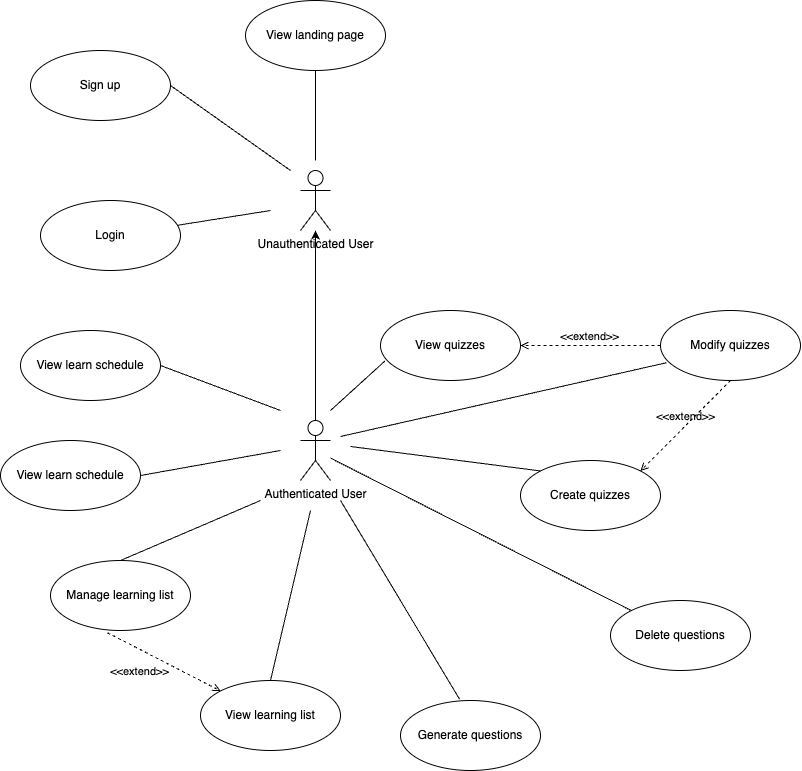
\includegraphics[width=0.8\textwidth, keepaspectratio]{figures/use-case.png}
    \caption{SpacedAce use case diagram}
    \label{fig:use-case}
\end{figure}

TODO - use case diagram and explanations
\chapter{Theoretical background}\label{ch:theoretical-background}

This chapter explores three key concepts that power the learning platform: the spaced repetition algorithm, large language models (LLMs), and the REST (REpresentational State Transfer). Spaced repetition is a learning technique that can help improve long-term retention by scheduling the learning material at increasing intervals \cite{ebbinghaus1964memory}. It is an evidence-based technique and is usually performed with flashcard-like methods, which makes it practical to implement into the learning platform. On the other hand, LLMs act as knowledge bases that generate targeted questions.

REST is an architectural style for distributed hypermedia systems, originally introduced by Roy Fielding~\cite{fielding2000} in his 2000 doctoral dissertation. Despite its widespread adoption in modern web development, it is worth exploring in detail here, particularly focusing on HATEOAS (Hypermedia as the Engine of Application State) - a less commonly understood principle that forms a crucial foundation for a concept discussed later in this thesis. By combining these techniques, the platform can create a tailored learning experience.

\section{Spaced Repetition}

Spaced repetition is a method of learning at semantic intervals. These intervals become longer as the studying process goes on. Initially, these intervals are short, usually a few hours long, and for a long time, they could even be multiple years long. The method's primary goal is to help the practitioner retain the information in long-term memory.

This method is the complete opposite of cramming; it is not trying to learn everything in the shortest possible time. It focuses on understanding the learning material for the long term by "re-learning" it repeatedly after increasing intervals. A German psychologist, Hermann Ebbinghaus, first described this learning technique in the late 19th century. In 1885, He published his research about memory and forgetting in his book On Memory~\cite{ebbinghaus1964memory}.

In his book, Ebbinghaus wrote about the \texttt{forgetting curve}, the idea of forgetting information at a predictable rate. He discovered that humans forget information rapidly faster after the first learning, but reviewing the information at strategic intervals helps slow it down. Figure~\ref{fig:forgetting-curve} visually shows the concept of \texttt{forgetting curve}. The first practical application of his theories was developed much later by German science journalist Sebastian Leitner in the 1970s.

\begin{figure}[!h]
  \centering
  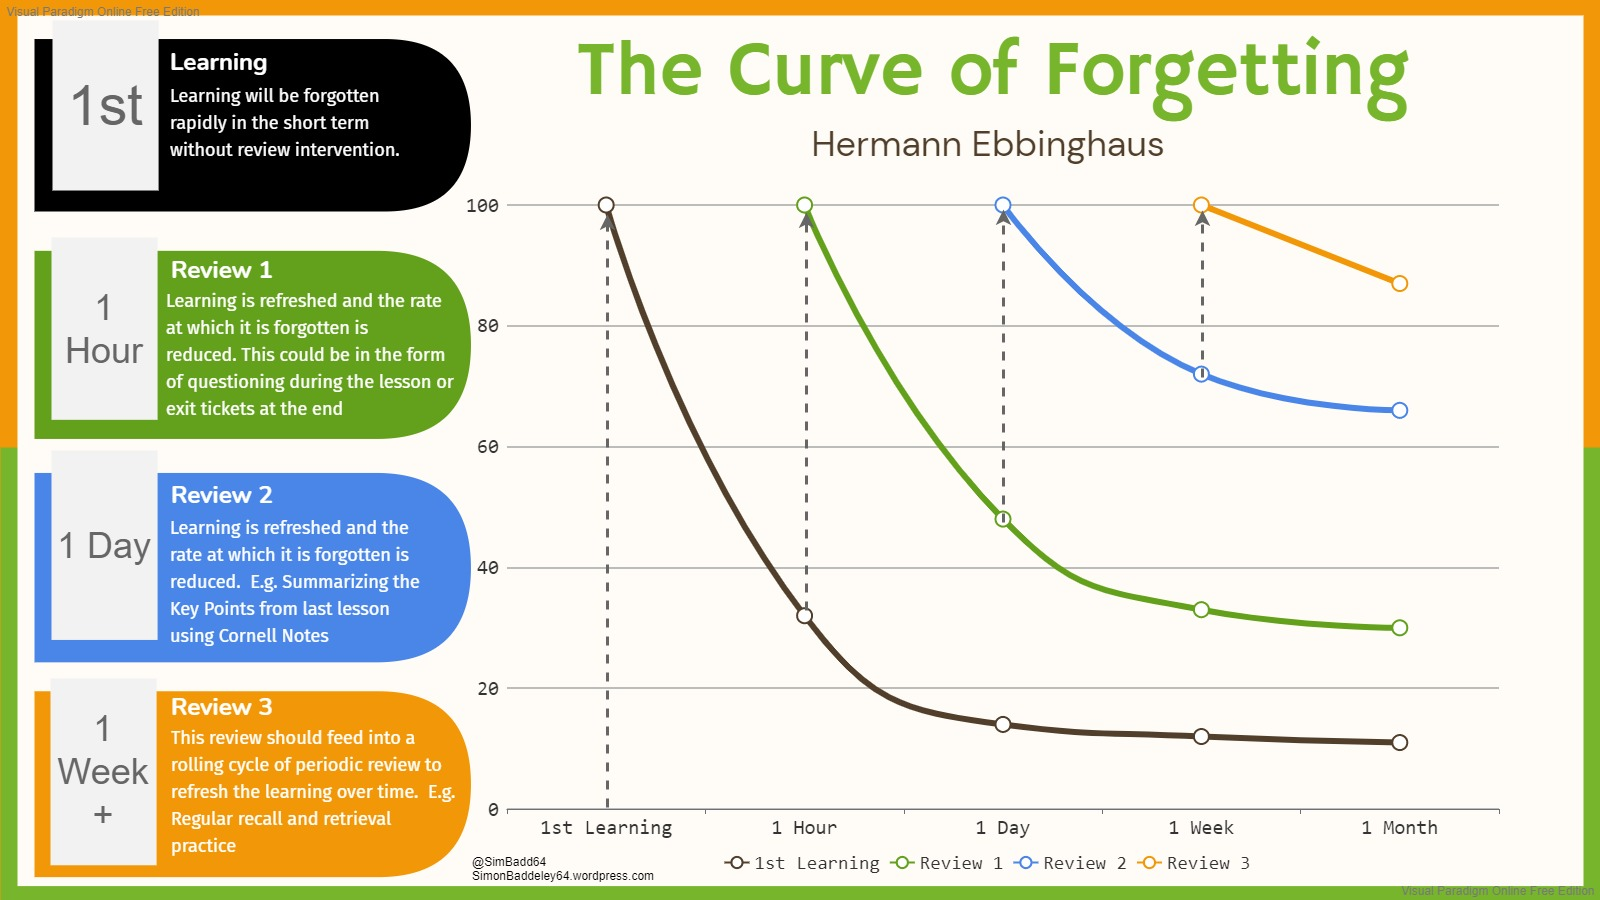
\includegraphics[width=0.8\textwidth, keepaspectratio]{figures/forgetting_curve}
  \caption{The Curve of Forgetting, created by: Simon Baddeley}
  \label{fig:forgetting-curve}
\end{figure}

Leitner's implementation is called the Leitner system \footnote{https://en.wikipedia.org/wiki/Leitner_system}. It is a paper-based method of using flashcards organized into numbered paper boxes. These paper boxes represent review intervals. When a question is answered correctly, it goes up by one, and when answered incorrectly, it goes down by one. Figure~\ref{fig:leitner-system} shows it visually.

\begin{figure}[!h]
  \centering
  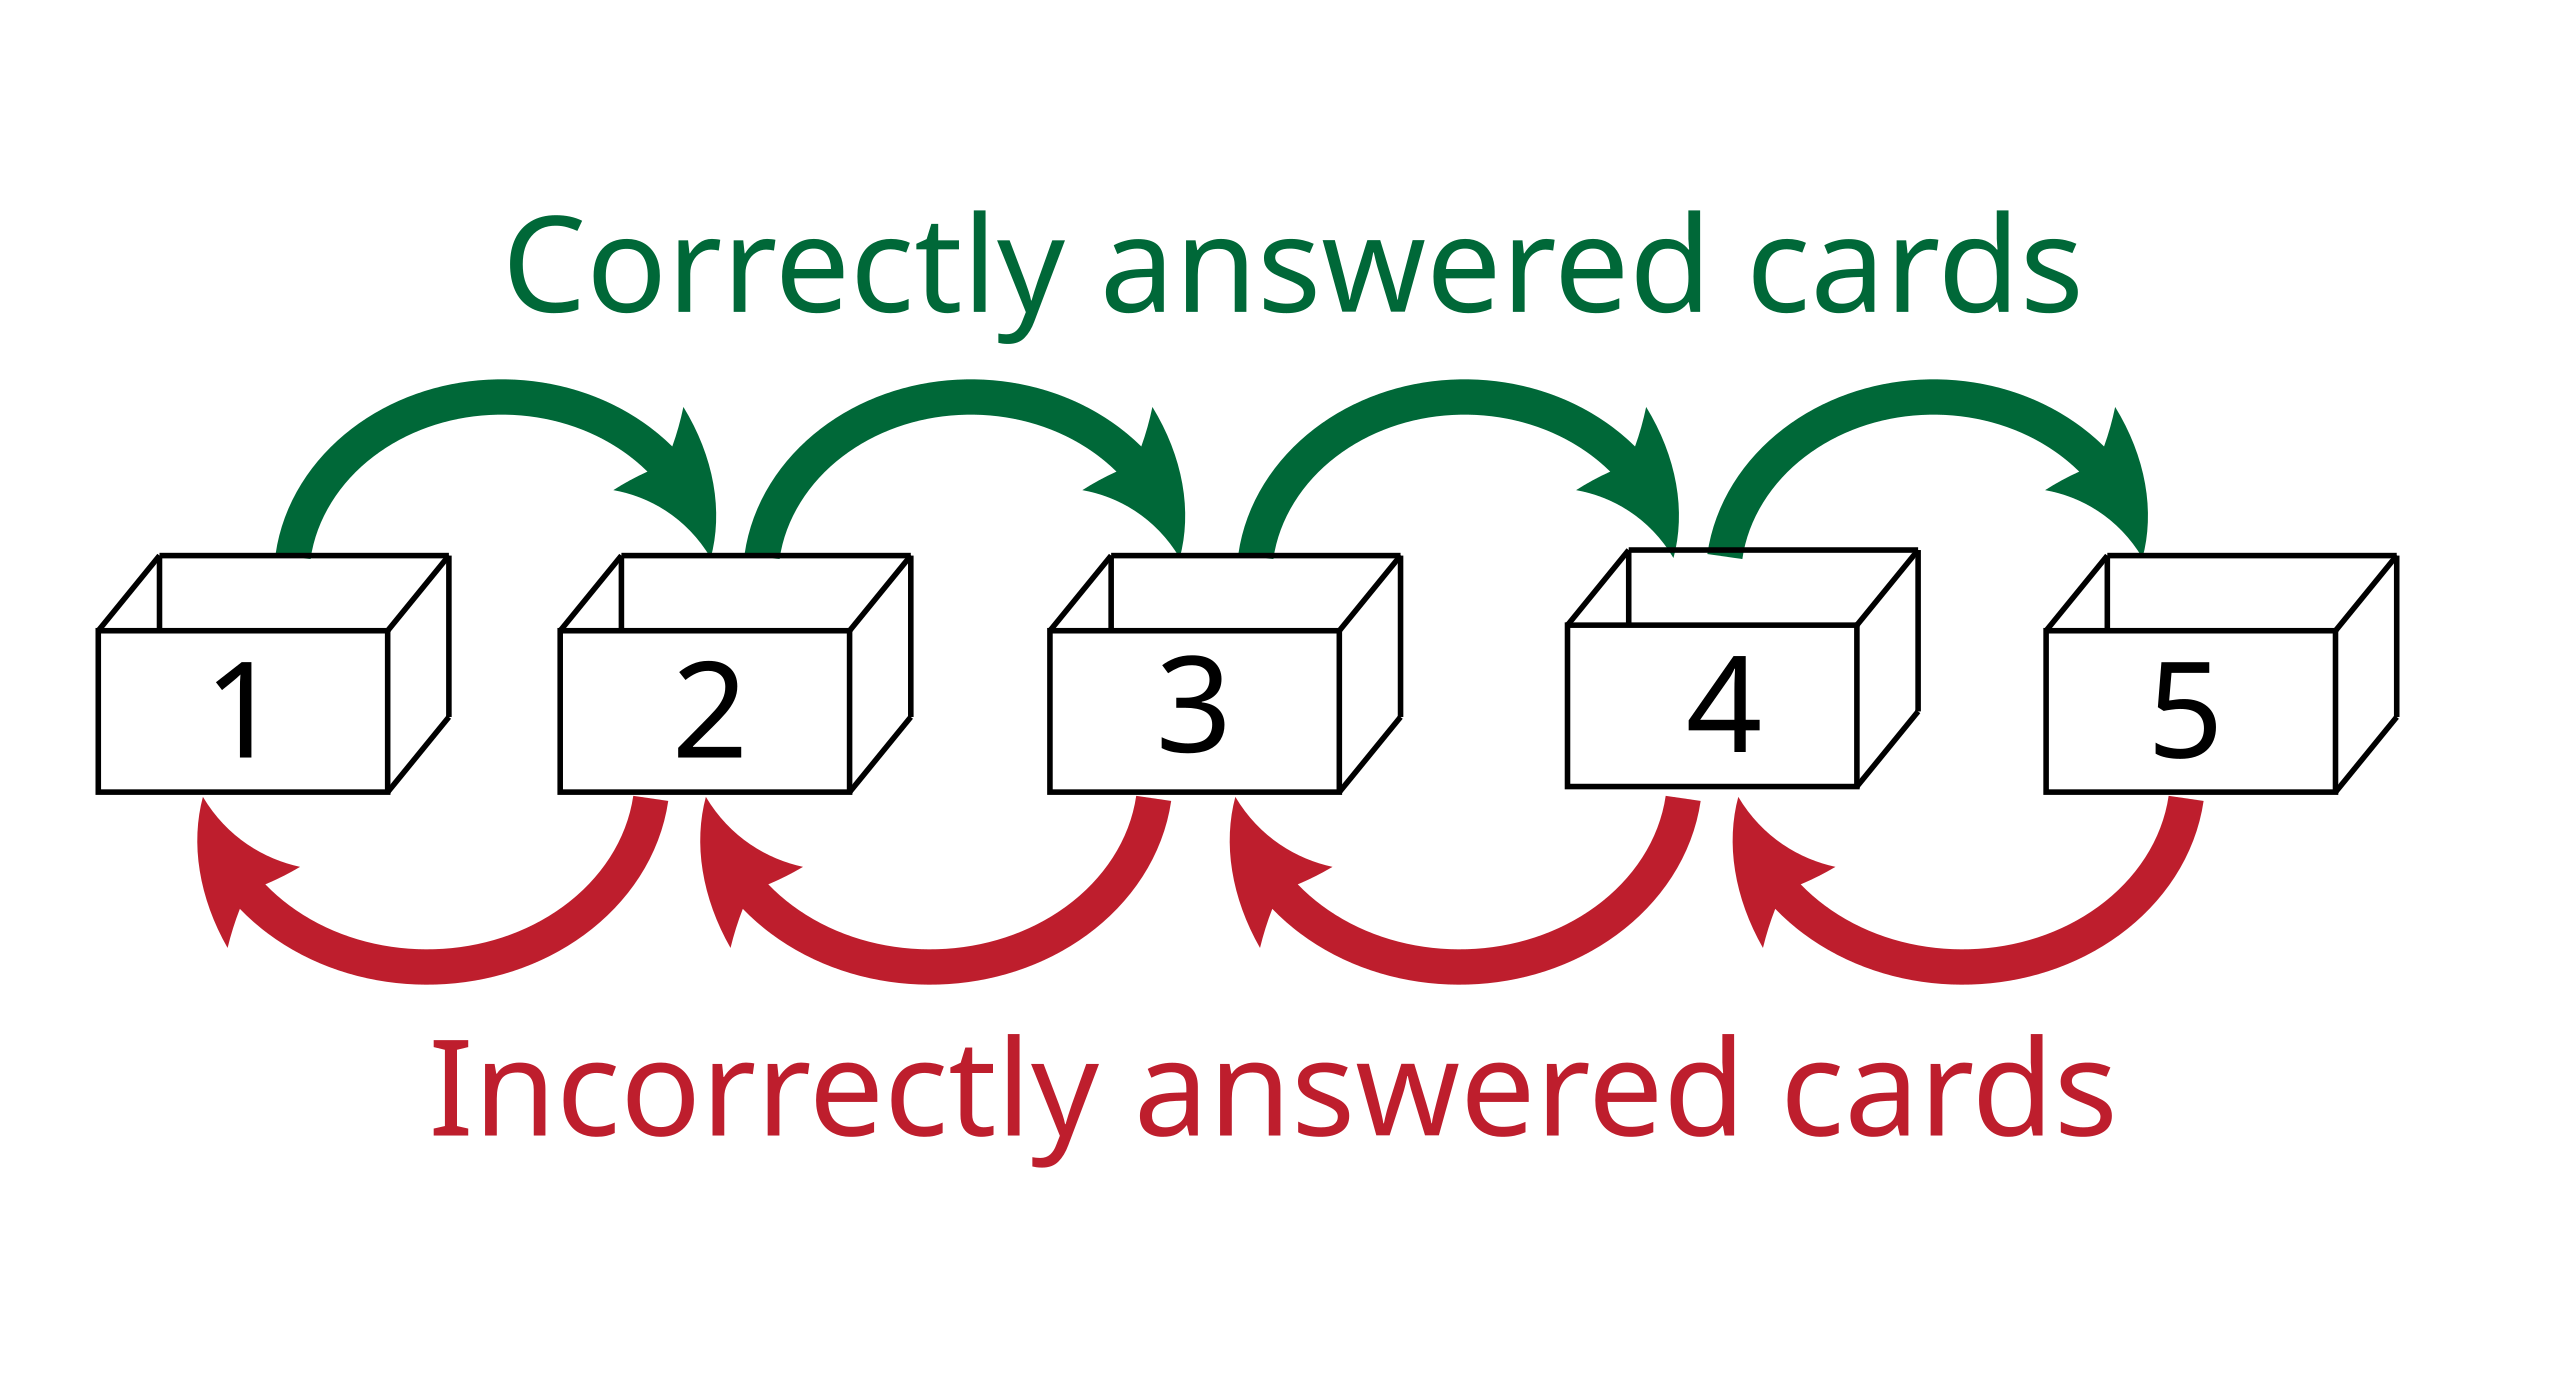
\includegraphics[width=0.8\textwidth, keepaspectratio]{figures/Leitner_system}
  \caption{Leitner system, source: Wikipédia}
  \label{fig:leitner-system}
\end{figure}

In 1987, a Polish computer engineer, Piotr Wozniak, created the first educational software implementing spaced repetition, called \texttt{SuperMemo} \footnote{https://www.supermemo.com/en}. His \texttt{SuperMemo} algorithm calculates the optimum interval for learning. The algorithm has evolved several times, using different metrics and parameters to determine the optimal interval. The current version of his algorithm is SM-17\footnote{https://supermemo.guru/wiki/Algorithm_SM-17}. For the platform, I implemented a prototype algorithm similar but simpler to his using similar parameters.

The core parameters of my algorithm are the following: \textt{score}, \textt{difficulty}, \textt{streak}, \textt{interval} and \textt{ease factor}.

\textbf{score}: The \texttt{score} is the score the user reached when answering the given question. It is a number between one and five.

\textbf{difficulty}: The \texttt{difficulty} of the question represents how challenging it is to remember the particular answer. It is used to adjust the review interval.

\textbf{streak}: The \texttt{streak} represents the number of successful consecutive recalls. It resets to 0 when the user struggles to answer correctly.

\textbf{interval}: The \texttt{interval} is the time between the reviews. It is calculated all the other from all the parameters. It increases exponentially based on user performance.

\textbf{ease factor}: The \texttt{ease factor} measures how easily and item is remembered over time. It increases for good performance and decreases for poor performance.

The concrete Go implementation is detailed at the \texttt{Spaced repetition algorithm} subchapter~\ref{subsec:spaced-repetition-algorithm}.

\section{Large Language Models}

"Large Language Models (LLMs) are advanced Artificial Intelligence (AI) systems that have undergone extensive training using large datasets in order to understand and produce language that closely resembles that of humans~\cite{buscemi2023comparative}."  These models can be used in various fields, e.g., education technology, healthcare, business, science, and software development. They provide a personalized user experience in these fields. Therefore, they are excellent for use on learning platforms like SpacedAce.

The core innovation of LLMs lies in the transformer architecture introduced by Vaswani et al. in 2017~\cite{vaswani2017attention}. Transformers improve over earlier neural networks because they use a self-attention mechanism. It allows the models to process entire sequences simultaneously, enhancing efficiency and performance. The transformer architecture consists of two main parts: encoder and decoder. The encoder processes and transforms the input into a high-dimension representation, while the decoder generates the output word-by-word using the encoder's output and the previously generated tokens. Figure~\ref{fig:encoder-and-decoder} shows an encoder and decoder architecture.

\begin{figure}[H]
  \centering
  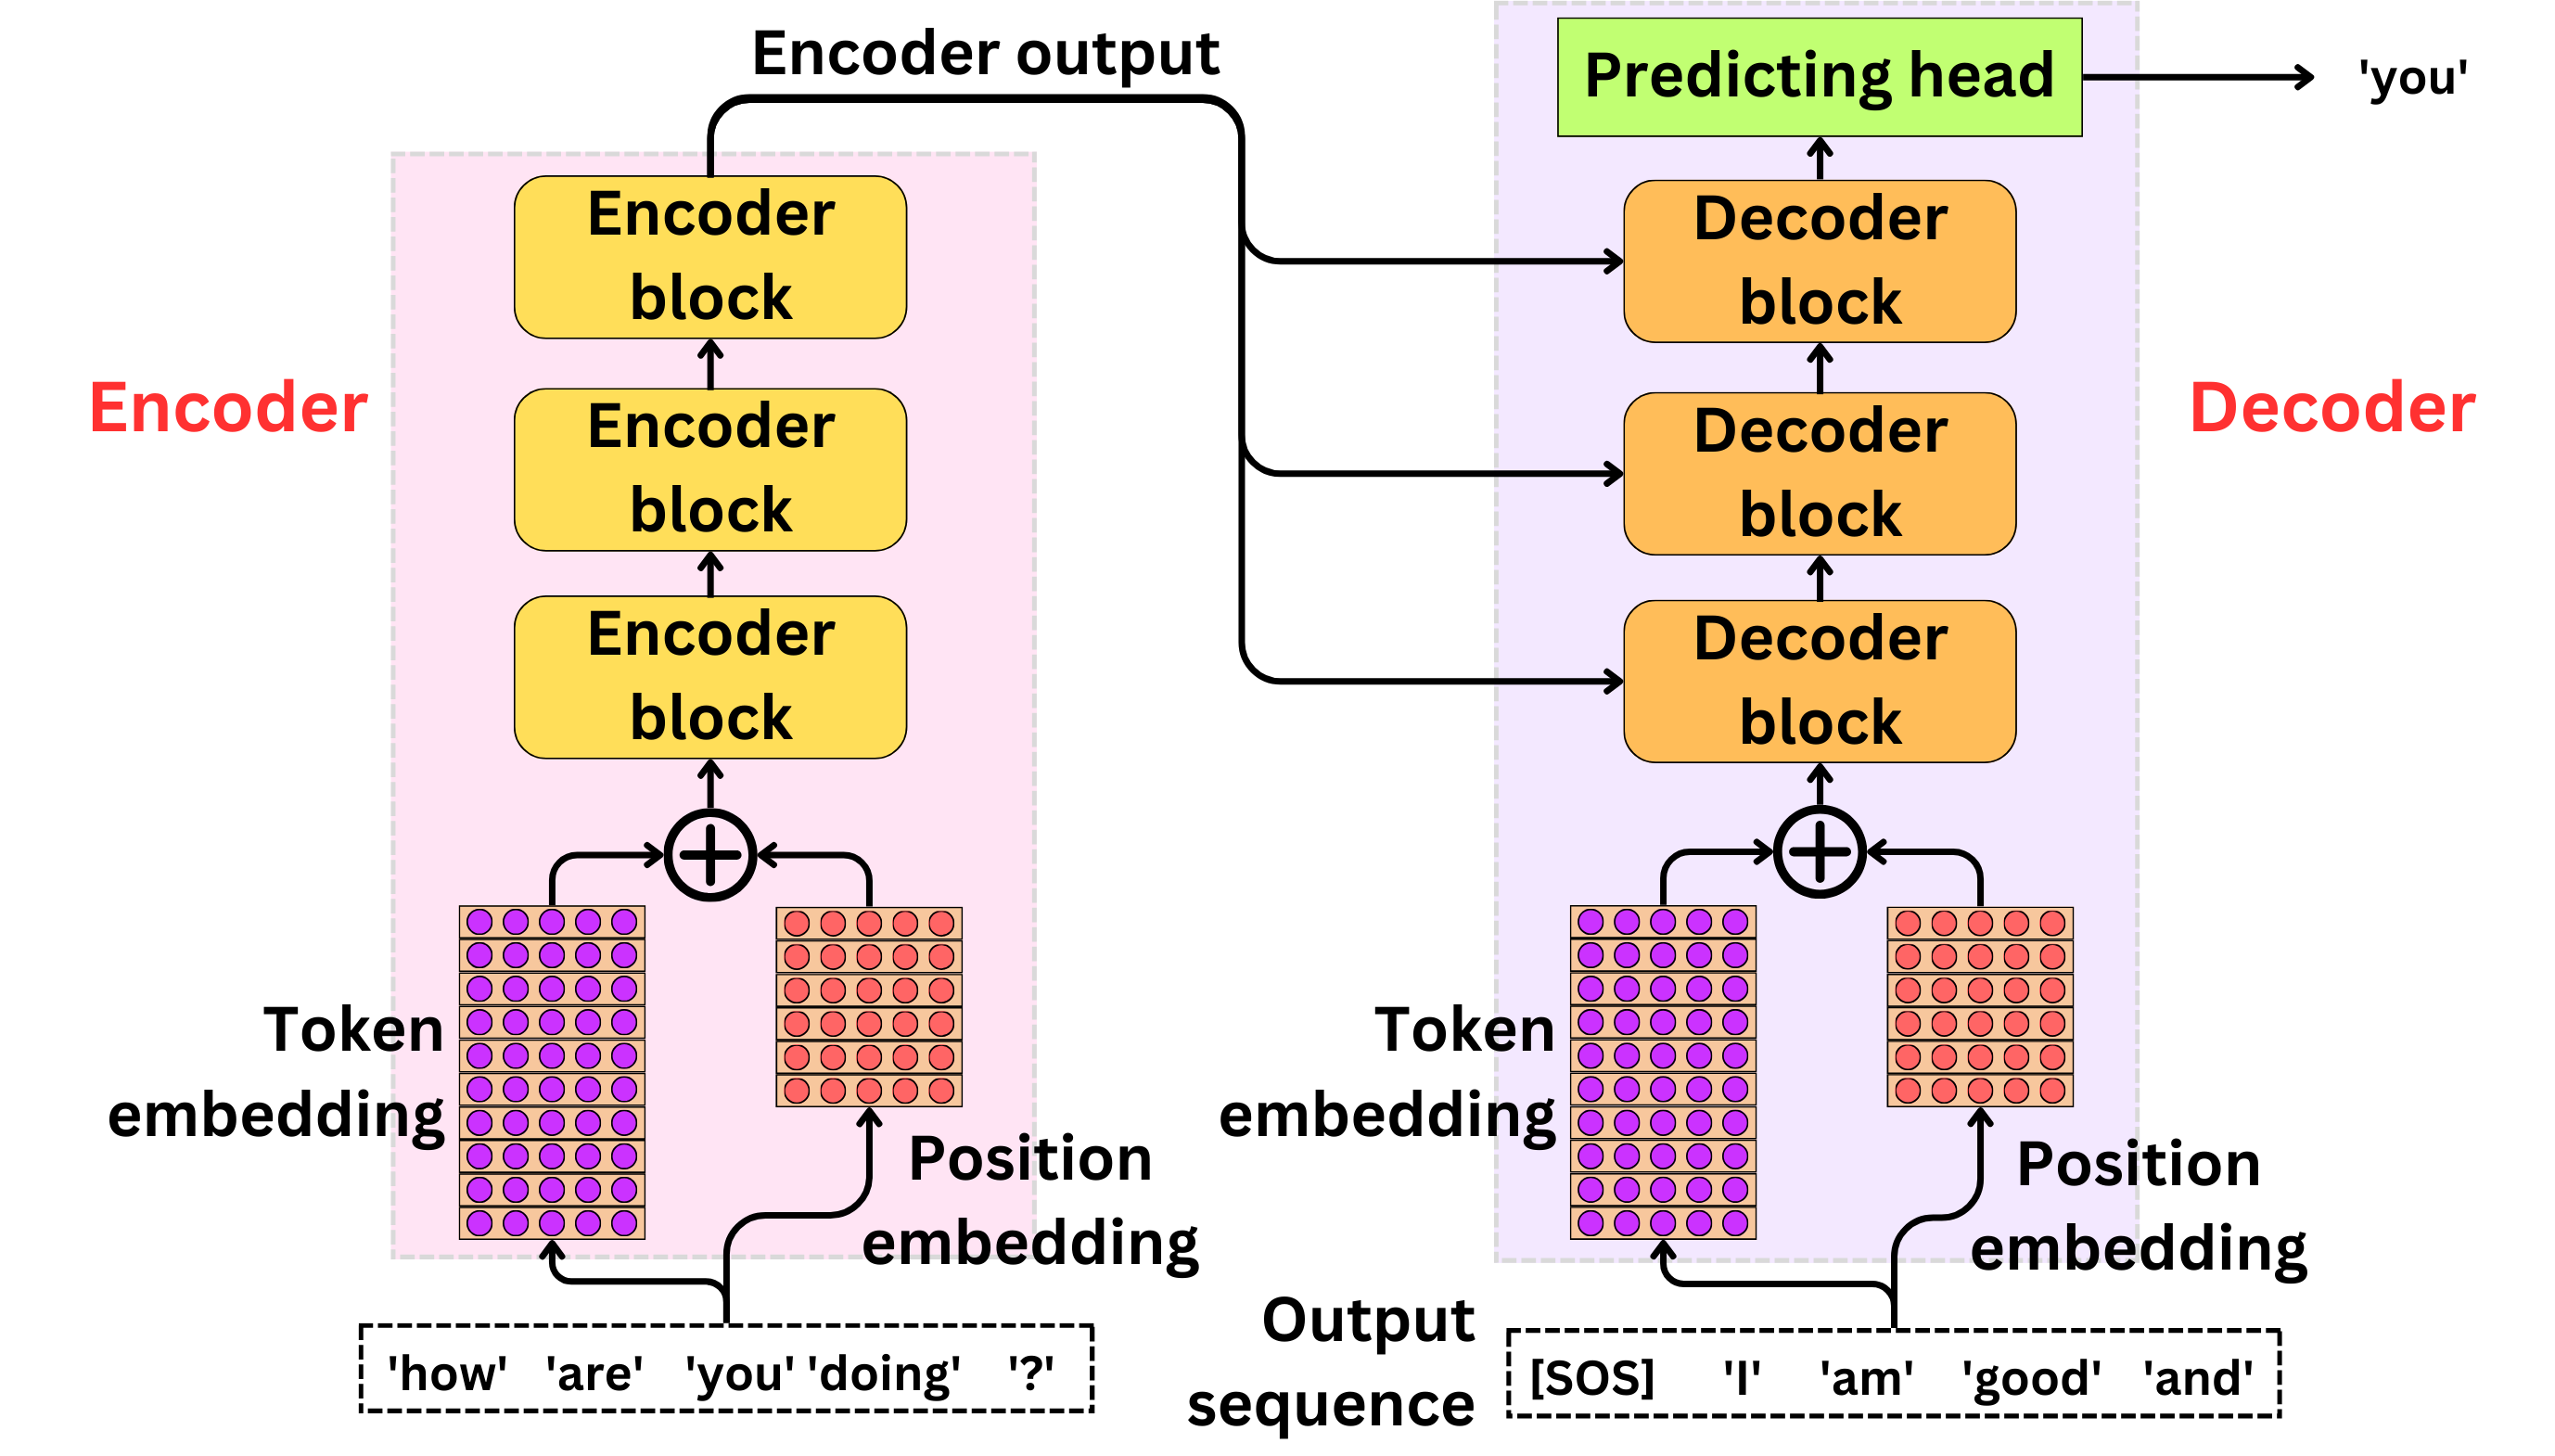
\includegraphics[width=0.8\textwidth, keepaspectratio]{figures/encoder-and-decoder.png}
  \caption{Encoder and decoder architecture, created by: Damien Benveniste \footnote{https://newsletter.theaiedge.io/p/understanding-the-transformer-architecture}}
  \label{fig:encoder-and-decoder}
\end{figure}

Key characteristics of modern LLMs include their ability to perform few-shot and zero-shot learning, meaning they can adapt to new tasks with minimal or no task-specific training~\cite{brown2020language}. Taking advantage of this feature, Máté finetuned a pre-trained \texttt{llama-3-8B-instruct1}\footnote{https://huggingface.co/meta-llama/Meta-Llama-3-8B-Instruct} model and crafted prompts with few-shot prompting technique for the platform.

\section{REST}

The REST architectural style has six guiding principles, all of which must be satisfied by a REST-ful service. Roy names them \cite[Chapter 5]{fielding2000}: Client-Server, Stateless, Cache, Uniform interface, Layered system, and Code-On-Demand. This principle describes how a REST service should look, what components it can have, and how these components can communicate. Developers mostly know these, but one of them, HATEOAS, usually needs to be remembered.

\subsubsection{HATEOAS}

HATEOAS is a small constraint that many people tend to forget. If we take the constraint strictly, most REST applications would not be REST applications. It is usually fine because most applications work differently than Fielding imagined in his dissertation back in the day. To comply with this requirement, each response must include hyperlinks to the accessed data and the available system actions, ensuring comprehensive and interactive user navigation. The listing~\ref{lst:hateoas} shows an example of a compliant response.

\begin{lstlisting}[caption=An HATEOAS response in JSON format,label=lst:hateoas, H]
{
  "accountId": "123456789",
  "accountName": "John Doe",
  "balance": 1500,
  "links": [
    {
      "rel": "self",
      "href": "http://examplebank.com/accounts/123456789",
      "method": "GET"
    },
    {
      "rel": "deposit",
      "href": "href": "http://examplebank.com/accounts/123456789/deposit",
      "method": "POST"
    },
    {
      "rel": "withdraw",
      "href": "href": "http://examplebank.com/accounts/withdraw",
      "method": "POST"
    }
  ]
}
\end{lstlisting}

One of the main ideas of HTMX is to be HATEOAS compliant. The website pages are generated dynamically on the server to contain the requested resource and all the actions available for the given resource. The server generates the page and adds HTMX requests to desired elements representing the actions.
\chapter{Technologies}\label{ch:technologies}

This chapter details the essential web technologies used to create the platforms. It starts by introducing Go and then continues with the Echo framework. It also shows the database libraries (SQLx and SQLC) used in the backend and templating language templ. Finally, it finishes by describing HTMX, the unique framework library.

\section{Go}
Go is a statically typed, compiled programming language created by three engineers: Robert Griesemer, Rob Pike, and Ken Thompson at Google. It first appeared in 2009 and gained popularity over the years. It was the 13. most popular programming language among the respondents of the 2023 Developer Survey\footnote{https://survey.stackoverflow.co/2023/} published by Stack Overflow\footnote{https://stackoverflow.com/}. Their methodology says They asked around 90,000 software developers from 185 countries around the world between May 8, 2023, and May 19, 2023.

\begin{figure}
    \centering
    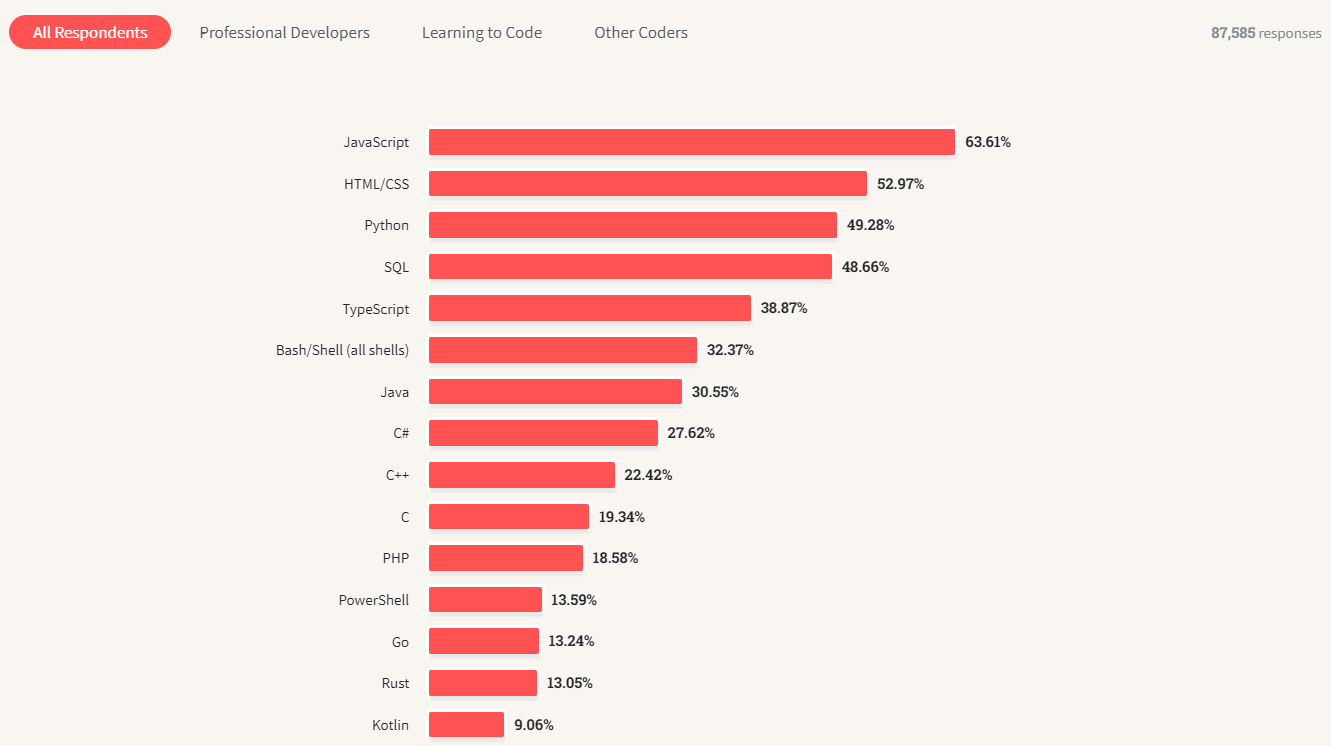
\includegraphics[width=160mm, keepaspectratio]{figures/go-stack-overflow.png}
    \caption{Most popular programming languages - 2023 Developer Survey by Stack Overflow}
\end{figure}

The language is designed to make programmers more productive in several fields, including  Web development, Cloud, Command Line (CLI) Applications, and DevOps, by offering modern features and a robust standard library. In most cases, you could write programs relying only on the standard library without using external dependencies. Nevertheless, the language ecosystem has a unique package management solution with an easy-to-use module system. You can download the packages from their package registry called pkg.go.dev\footnote{https://pkg.go.dev/} or even directly from a code repository like GitHub\footnote{https://github.com/}.

\subsection{Key features of Go}

The Go language has many features. I will introduce some of the most important ones in the following sub-sections: simplicity, readability, composition over inheritance, concurrency, tooling, and performance. 

\subsubsection{Simplicity}

The Go language is designed with simplicity in mind to address the complexity issue in software development. This feature was achieved by omitting common features in other languages and minimizing syntax. 

For example, Go only includes a \textbf{for} loop, leaving out constructs like \textbf{while} and \textbf{do-while}, and it lacks inheritance, a feature typical of object-oriented languages. Until a few versions ago, it was not even possible to write generic functions.

\subsubsection{Readability}

The language's minimal syntax makes it easy to read and understand, even for those who are not familiar with it firsthand. It can be a bit verbose compared to other languages, but this helps clarify the intent behind the code faster.

\subsubsection{Composition over inheritance \cite{gamma1994design}}

Composition over inheritance is a commonly applied design principle that promotes combining smaller, reusable components to achieve functionality rather than relying on hierarchical inheritance structures. The language does not have an inheritance feature at all. This approach reduces tight coupling and helps write more easily maintainable code.

\subsubsection{Tooling}

The language has an extensive set of tooling, including a compiler (go build), a package and dependency manager (go mod), a testing tool (go test), a code formatter (go fmt), and a language Server called (gopls\footnote{https://pkg.go.dev/golang.org/x/tools/gopls}). Most of them are deeply integrated into the ecosystem and come by default. Utilizing them, the developer could experience a fast, smooth, and efficient workflow experience.

\subsubsection{Concurrency}
Go features a simple yet robust concurrency model. It provides goroutines, lightweight threads managed by the Go runtime, and channels, facilitating safe and efficient communication between goroutines. It has an explicit syntax and is straightforward even for beginners, as the listing \ref{lst:goroutine} shows.

\begin{lstlisting}[caption=Calling a normal function as a goroutine,label=lst:goroutine, float]
package main

import (
	"fmt"
)

func normalFunction() {
	fmt.Println("I am a normal function")
}

func main() {
	// normal call
	normalFunction()

	// call as a goroutine
	go normalFunction()
}

\end{lstlisting}

\subsubsection{Performance}

Go is designed to be high-performance. This has been achieved by combining the speed of compiled programs with garbage-collector-based memory management. In addition, the concurrency model and the use of goroutines help to write fast and scalable applications.

\subsection{Advantages of using Go}

Go offers practical benefits that enhance software development and deployment. Its fast compile times speed up the development process, allowing more and faster iterations. Additionally, Go's ability to produce a single executable binary file simplifies the deployment process, even for different platforms.

Furthermore, Go's runtime includes a well-optimized garbage collector, which helps write applications with fewer memory leaks. Go's approach to treating errors as values is a simple and robust error-handling technique that forces developers to handle errors explicitly to reduce runtime failures.

\subsection{Disadvantages of using Go}

As with everything, Go has some disadvantages. The error-handling approach can be verbose and contain boilerplate code, as the developers must explicitly check and handle the errors.

I mentioned before that the language lacked generic functions and data types. It caused a lot of reimplementation of basic logic, e.g., the developers had to implement a linear search for every number type when deciding whether a slice contained it. The developer community still managed to convince the creators, and in 2022, version 1.18\footnote{https://go.dev/blog/why-generics} was released, which implemented this feature in some form, and since then, more and more features based on it have been released.

The language is not a multi-paradigm programming language; thus, you cannot write code in an object-oriented or functional style. This can be a deal breaker for those used to other modern languages like JavaScript, Python, Java, etc.

\section{Echo framework}

"Echo is an extensible, minimalist web framework for Go. It has a highly optimized router, offers a rich collection of middleware functions, and is one of the simplest solutions for writing a scalable web application"\cite{EchoFramework}.

\subsection{Key features}

Key features include automatic TLS, HTTP/2 support, a middleware system, and seamless integration with several templating engines. 

Echo's design centers on middleware, which enables developers to add authentication, logging, and other custom features with minimal configuration. The framework supports the creation of custom middleware, allowing developers to inject their logic into the request-handling pipeline. 

Besides the standard templating engine (html/template), Echo supports multiple third-party solutions such as htmgo\footnote{https://htmgo.dev/}, Jet\footnote{https://github.com/CloudyKit/jet}, and templ\footnote{https://github.com/a-h/templ} for generating dynamic HTML pages. Initially, this application used the standard library, but I later migrated the code to use the more type-safe solution templ, which I continue to use.

\subsection{Example}

Creating and starting an HTTP server with Echo requires three simple steps:
\begin{enumerate}
\item Instantiating an Echo instance
\item Registering middlewares and routes
\item Starting the server
\end{enumerate}

Listing~\ref{lst:echo-http-server} demonstrates these steps with code from the application:

\begin{lstlisting}[caption=Starting an Echo HTTP server,label=lst:echo-http-server, float]
package main

import (
    "github.com/labstack/echo/v4"
    "net/http"
)

func main() {
    // Instantiate the Echo
    e := echo.New()

    // Register a route handler that responds with an HTML page for requests coming from path /
    e.GET("/", func(c echo.Context) error {
        return render.TemplRender(c, http.StatusOK, pages.IndexPage())
    })

    // Start the server listening on the port 42069
    e.Start(":42069")
}

\end{lstlisting}

\section{SQLx and SQLc}

SQLx and SQLc are popular tools for working with SQL databases in Go. They take distinct approaches to handling database operations. The first one follows a more traditional approach by using type structures with tags and calling prepared statements. This methodology is known and commonly used in other languages and frameworks like Java Spring's Hibernate library\footnote{https://docs.spring.io/spring-framework/reference/data-access/orm/hibernate.html}. In contrast, the other generates the code directly from SQL schemas and queries containing prepared statements, ready-to-use data types, and type-safe functions for database access.

During the design phase, I used SQLx in the backend for database handling because its approach felt familiar based on my previous experiences. This familiarity was essential to me, given that most other tools used to build the platform were entirely new. However, later in the development, I learned about the SQLc library and tried it out. Half of the code still uses SQLx, but the other half is implemented with SQLc. As I became familiar with the Go ecosystem and its coding styles, I found SQLc more convenient, so I plan to migrate the entire codebase to SQLc.

\subsection{SQLx implementation approach}
As I mentioned, SQLx follows a traditional approach. The developers must create type structures with special tags called "struct tags" and write prepared statements with SQL queries within. They must also write Go code that calls the library and parses the results. This approach can be a better fit for developers who need more control and manual optimizations over the queries.

\subsection{SQLc implementation approach}
On the other hand, SQLc is a code generator with pros and cons. It is not just a library but a CLI program with various helping tools, and it supports other languages besides Go. 

The developers must write the SQL schema with special comments for the generator and the query. The compiler generates the proper data types, mappings, and type-safe functions that execute the desired query. To work like this, the compiler must have a simple yet easily extensible configuration file that describes the type conversions and the coding style in some sense. This approach is better for developers who prefer hiding complexity behind code generation or have to work on the same data model in different environments.

\section{templ}

The templ is a reasonably new, upcoming templating language library and CLI tool that helps create dynamic HTML fragments type-safely. It has a special JSX-like syntax, which became popular in the JavaScript ecosystem but uses a combination of Go and HTML. It is built on Go's standard templating solution, offering a better developer experience with a friendly syntax, convenient-to-use tools, and less error-prone, type-safe code generation.

\subsection{How does it work?}
Thus, it is a code-generation tool that allows for language extension with special syntax. In the world of templ, everything is a component written in a particular templ function in Go. These functions return templ components that render HTML text and can contain HTML code with some Go logic. The component functions have named and typed parameters like others, making them fully type-safe and compatible with code completion tools. Figure \ref{fig:templ-generation} shows the process of code generation from templ code.

\begin{figure}[!h]
    \centering
    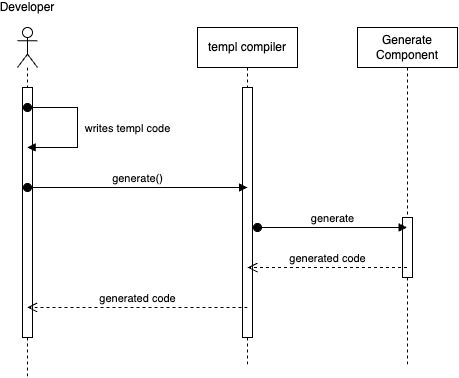
\includegraphics[width=0.8\textwidth, keepaspectratio]{figures/templ_sequence_generation.drawio.png}
    \caption{Code generation with templ compiler}
    \label{fig:templ-generation}
\end{figure}

Written code must follow strict coding rules and styles to generate the code called and used by the backend frameworks to render the page. The CLI contains a language server for code completion and syntax highlight, a code formatter, and a code generator tool. Figure \ref{fig:templ-rendering} shows the process of rendering a templ component.

\begin{figure}[!h]
    \centering
    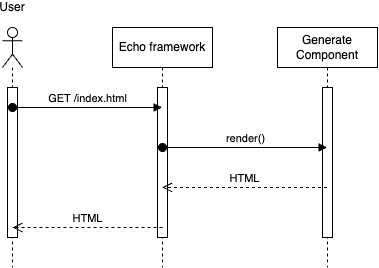
\includegraphics[width=0.8\textwidth, keepaspectratio]{figures/templ_sequence_render.drawio.png}
    \caption{Rendering templ component}
    \label{fig:templ-rendering}
\end{figure}

\section{HTMX}

HTMX is a tiny JavaScript library that allows developers to write server-rendered web applications primarily using HTML attributes. It enables HTML elements to handle advanced behaviors, eliminating or minimizing the need to write JavaScript code. It also complies with the REST constraint HATEOAS, as the returned HTML always contains the available actions for the requested resources.

One of the main goals is to create a SPA-like (single-page application) experience with the speed of server-rendered dynamic web pages. The difference between this and a traditional web application is the type of response. The communication is still based on HTTP, and the browser sends data in the known formats (URL, HTTP header, and HTTP body, even in JSON format), but the reactions are in HTML texts instead of JSON (or XML). The library is responsible for processing the HTML and updating the desired parts of the application based on the responses.

\subsection{Common HTMX attributes}

HTMX is like an extension of HTML, with 15 to 20 custom attributes that define how to process outgoing requests and incoming responses. The following ones are used the most.

Each HTTP method has attributes related to it: \textbf{hx-get}, \textbf{hx-post}, \textbf{hx-put}, \textbf{hx-patch}, \textbf{hx-delete}. Each one has one parameter: the URL where the request has to be sent when the actions happen. The listing \ref{lst:htmx-logout} shows performing a POST request to /logout on the default action of a button.

\begin{lstlisting}[caption=Preforming an \textbf{hx-post} request,label=lst:htmx-logout, float]
<button hx-post="/logout">Logout</button>
\end{lstlisting}

By default, on form submission, input value change, and button click, an HTMX request is performed when the method and URL are set. But there is a way to modify the default action trigger with \textbf{tx-trigger} attribute. It supports changing the event and allows the modifier to fine-grain the behavior, e.g., modifying an event, setting a delay, adding a throttle time, or filtering a key. The listing \ref{lst:htmx-trigger} shows performing a request on blur event with 300 ms of delay time.

\begin{lstlisting}[caption=Custom HTMX trigger,label=lst:htmx-trigger, float]
<input 
	id="data"
	name="data"
	type="text"
	hx-post="/update"
	hx-trigger="blur delay:300ms">
</input>
\end{lstlisting}

Some attributes define the process of the response. The two most common are \textbf{hx-target} and \textbf{hx-swap}; the first tells the library which element to swap, and the other tells how to do it. The target can be set by referring to the ID of the HTML element or using a CSS selector with special modifiers like \textbf{closest}, \textbf{next}, and \textbf{previous}. The other property tells how to do it, for example, changing the element's content, changing the whole element, and inserting before/after the target. The listing \ref{lst:htmx-target} shows a request, which response is replacing the element with id \textbf{\#page}.

\begin{lstlisting}[caption=Setting HTMX target,label=lst:htmx-target, float]
<a 
	hx-get="/home"
	hx-target="#page"
	hx-swap="outerHTML">Home
</a>
\end{lstlisting}

\subsection{Other attributes}
There are some cases when the website needs more complex logic, such as modifying multiple parts, sending additional data to the server, or doing client-side validation. HTMX offers solutions to all of them.

There are various methods to send data to the server, such as including it in the HTTP header or using the values from <input /> tags with \textbf{hx-include} or \textbf{hx-vals}.

If the application consists of several pages, navigation between them is necessary. This can be done with HTMX requests, in which the server sends not only the page but also the updated navigation bar. A request will cause the new page to appear and the navigation bar to be updated accordingly. This can be easily implemented with HTMX out-of-band requests and tags. The listing \ref{lst:htmx-oob} shows the request for a page and responses to the new page with the updated navigation bar.

\begin{lstlisting}[caption=Navigation with HTMX out-of-band request,label=lst:htmx-oob, float]
// The initial navigation bar
<nav
    id="navigation-bar"
    hx-target="#page"
    hx-swap="outerHTML"
>
    <a class="active" hx-get="/pages/1">Page one</a>
    <a hx-get="/pages/2">Page two</a> // the user clicks here
    <a hx-get="/pages/3">Page three</a>
</nav>

// the response containing the new page and an updated navigation bar
<div id="page">
    // Content of page two
</div>
<nav
    id="navigation-bar"
    hx-swap-oob="outerHTML:navigation-bar"
    hx-target="#page"
    hx-swap="outerHTML"
>
    <a hx-get="/pages/1">Page one</a>
    <a class="active" hx-get="/pages/2">Page two</a> // .active class is applied
    <a hx-get="/pages/3">Page three</a>
</nav>

\end{lstlisting}

Doing client-side validation, getting a prompt, or getting a confirmation from the user before sending a request, is easy; it just needs setting \textbf{hx-validate} and \textbf{hx-prompt} or \textbf{hx-confirm} attributes, respectively.
\chapter{Design}

This chapter details the platform's architecture. It begins with an overview of the architecture and a concise description of its key components. It then provides examples of how these components are deployed and interact with each other, which are covered in detail and displayed with diagrams. The following sections will go deeper into each component.

\section{System Architecture}

\subsection{High-level system architecture}

The platform consists of five main parts: the front end, back end, database, LLM-API, and the AI model, as the figure \ref{fig:high-level-architecture} shows. Each is containerized and can be deployed independently to scale as needed.

\begin{figure}[!h]
    \centering
    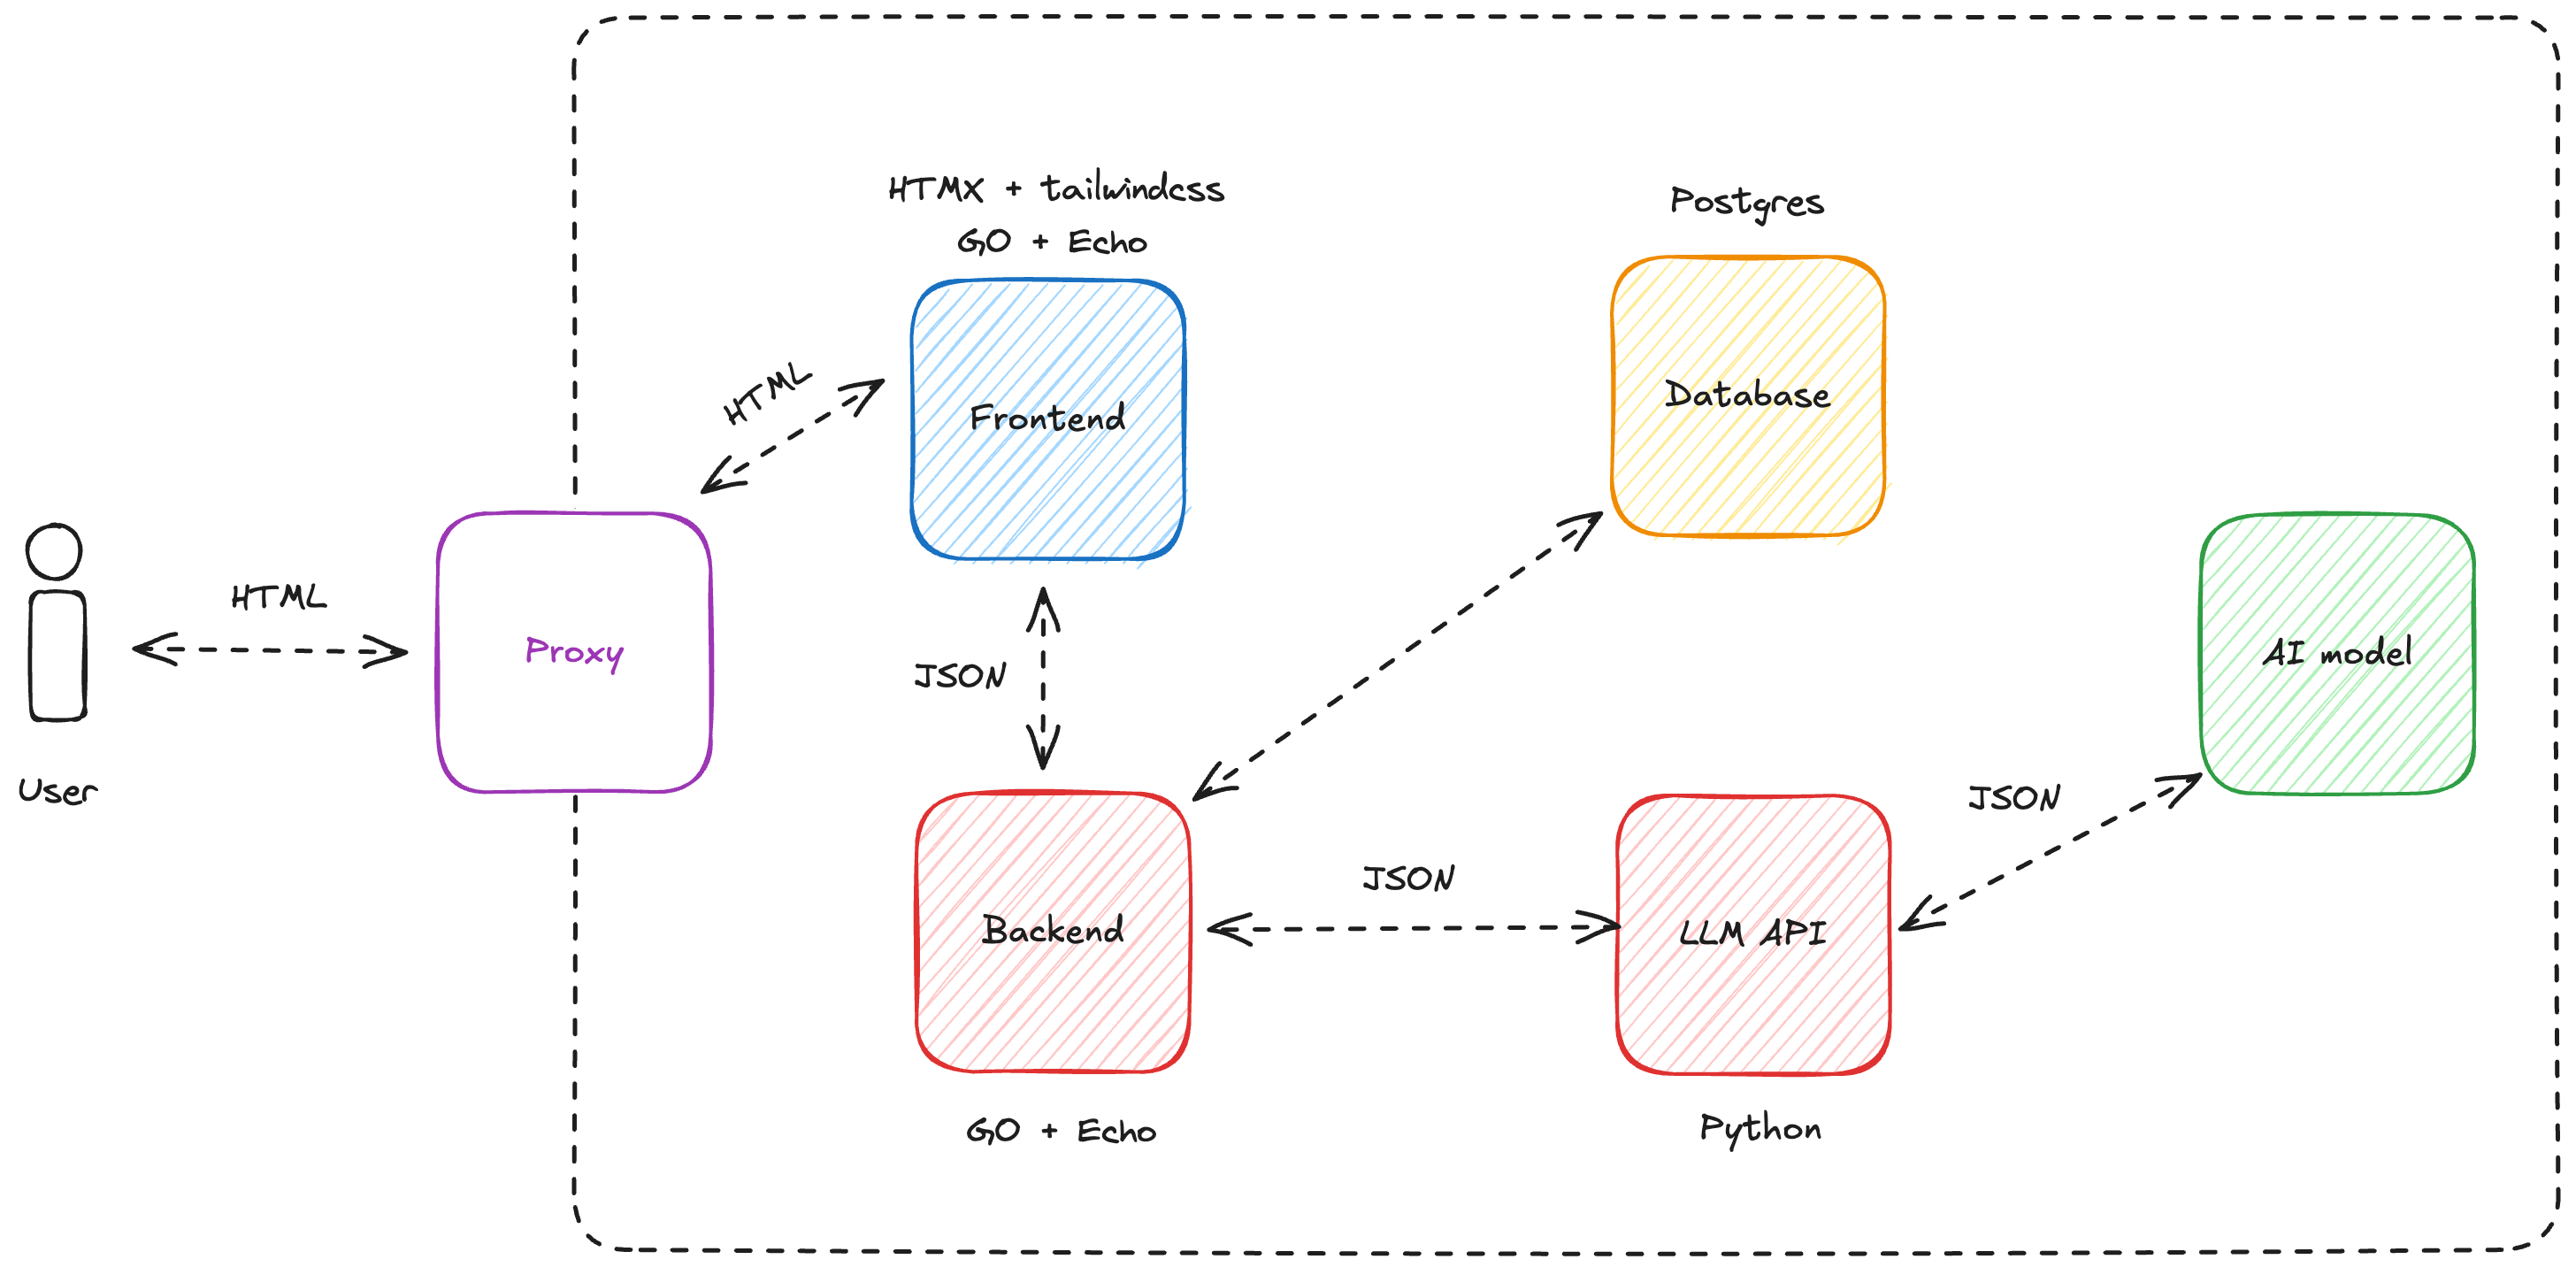
\includegraphics[width=0.8\textwidth, keepaspectratio]{figures/high-level-architecture.png}
    \caption{High-level system architecture}
    \label{fig:high-level-architecture}
\end{figure}

The frontend server is the part of the platform that users interact with directly. It's built as a server-rendered HTMX application using the Go programming language and the Echo framework. As the main entry point to the platform, it processes user inputs, communicates with the backend service, and provides content to users.

The backend is also written in Golang using the Echo framework. It is a regular REST application that communicates with HTTP requests. It brings together the different parts of the application and is responsible for the platform's business logic.

The database is Postgres, a popular, open-source relational database software. It stores all the data so the platform can work seamlessly. This component only communicates with the backend service.

The LLM API component is a unified interface for accessing the AI model. It is a small Python web application with a REST interface for more accessible communication. It contains prompts and question generation-related business logic. The component enables the platform to integrate different AI models or change between them on the fly.

The AI model component is a small application containing the question generator LLM. Máté Debreczeni fine-tuned the pre-trained llama-3-8B\footnote{https://huggingface.co/meta-llama/Meta-Llama-3-8B} model for the platform on a custom dataset he created from Wikipédia articles \footnote{https://en.wikipedia.org/wiki/Wikipedia:Vital_articles}. He aims to train a model that generates better-quality questions in the given format than the starter model.  

\subsection{Example component interaction}

Figure \ref{fig:component-interaction} shows an example interaction between the components through a question generation. This interaction is the primary interaction between the components and utilizes all of them.

\begin{figure}[!h]
    \centering
    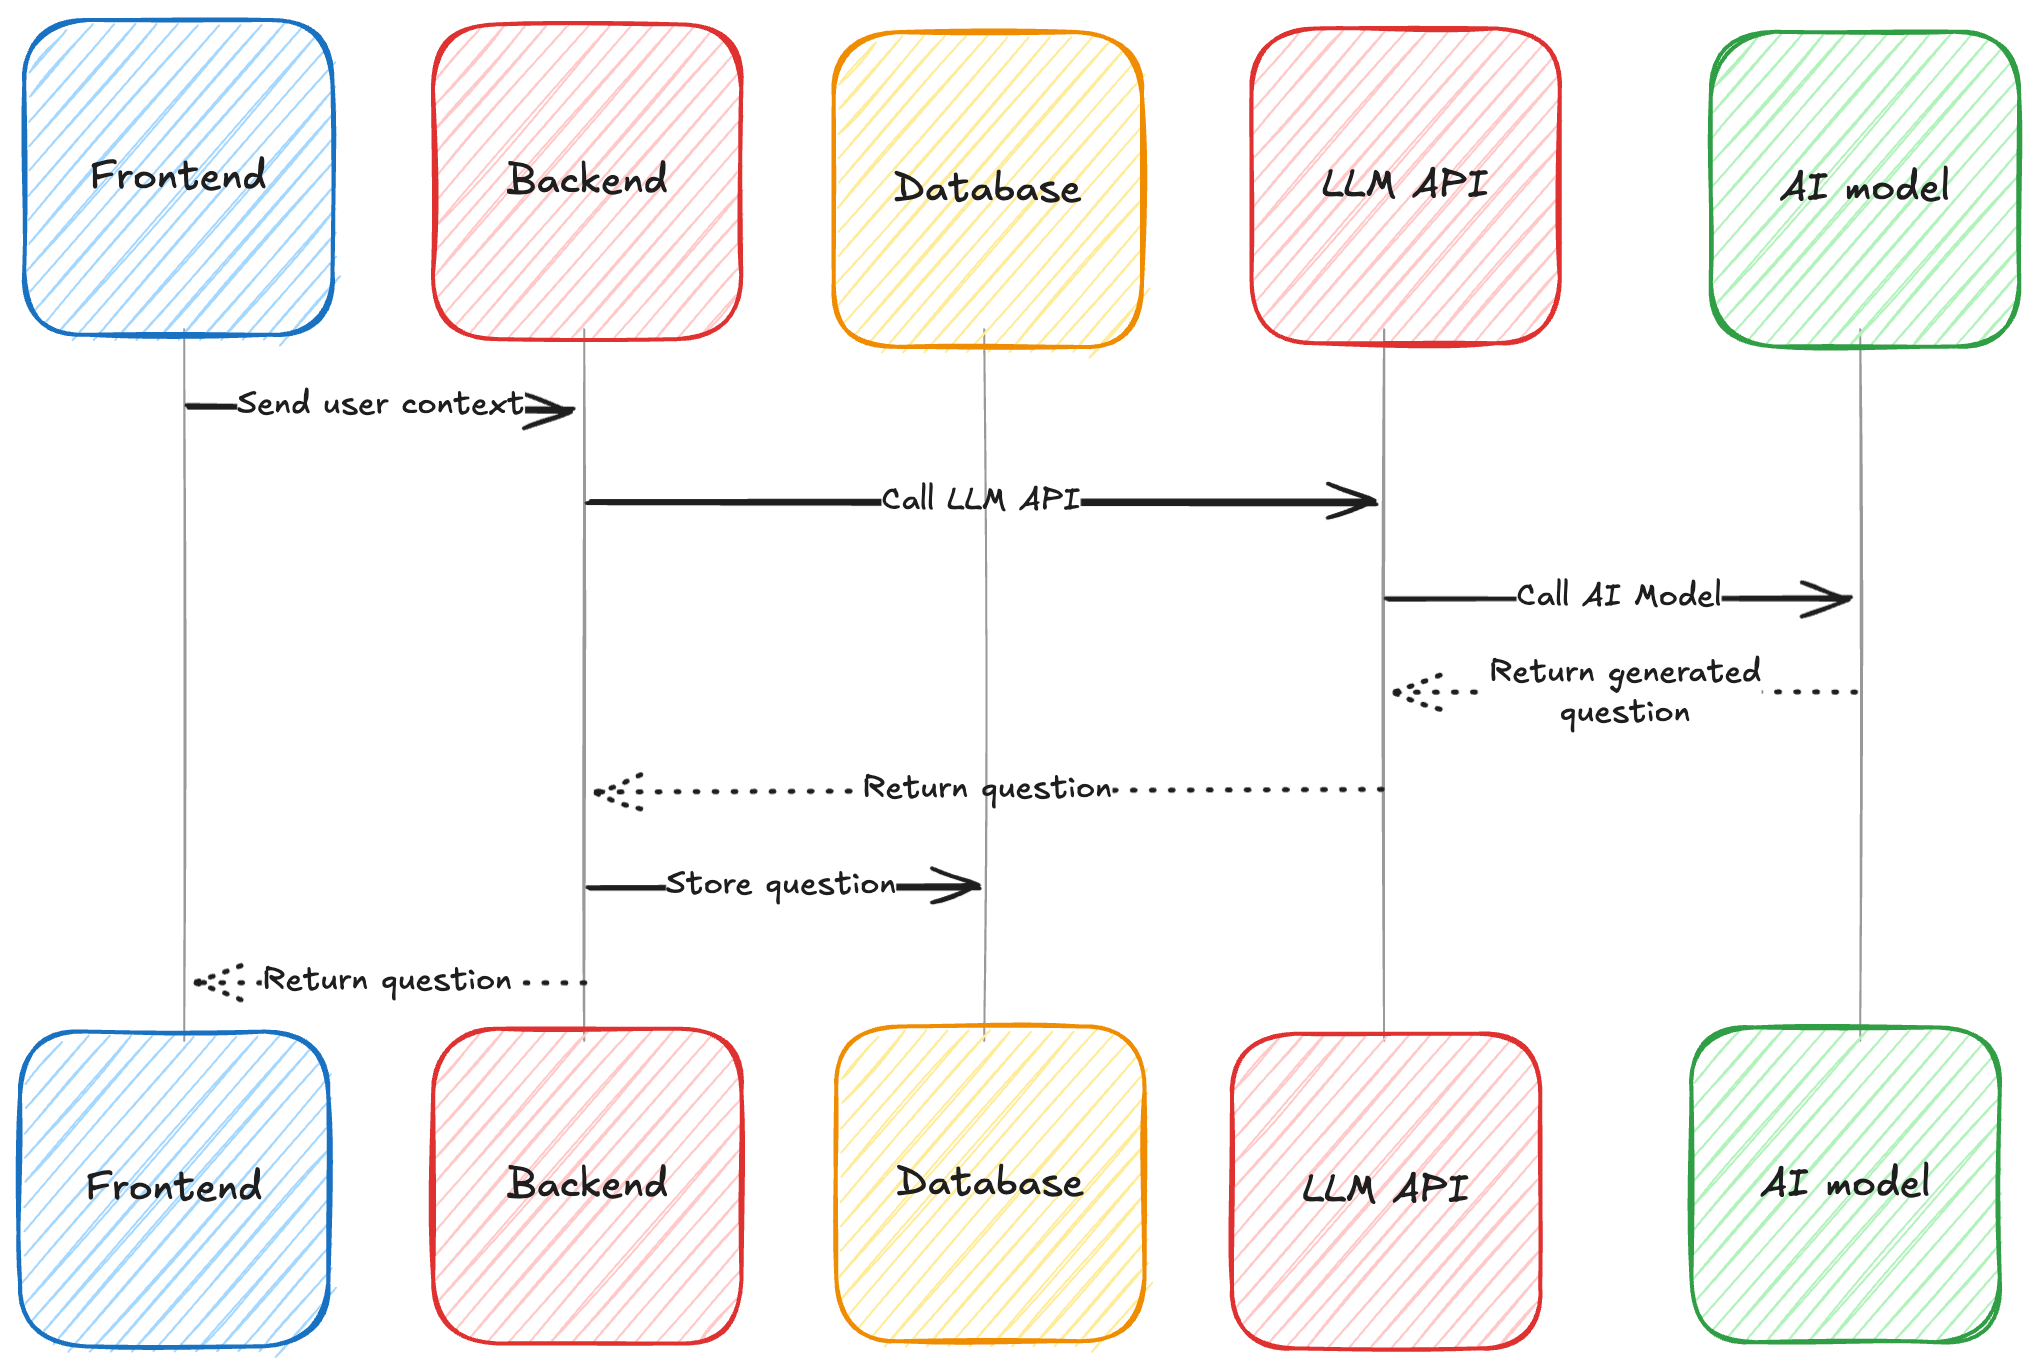
\includegraphics[width=0.8\textwidth, keepaspectratio]{figures/component-interaction.png}
    \caption{Component interaction: Question generation}
    \label{fig:component-interaction}
\end{figure}

Users submit their context to the frontend server, which validates the input and sets parameters like question type and quiz ID. The frontend calls the backend's proper endpoint with these parameters. The backend also validates the request and calls the LLM API to generate the question. The LLM API delegates the generation to the AI model through a request containing a pre-created prompt. This question is returned to the backend, where additional data is added and saved to the database. Finally, the backend returns the question to the frontend for display to the user.

\subsection{Deployment design}

Containerization is a crucial part of platform development and deployment. From the start, all the components were containerized with Docker for easier development and to ensure they worked on other machines. Máté worked on the AI model and the LLM API, and I worked on the other parts. Both of us used different operating systems, software, and tools. Without this method, we could not have worked together as efficiently as we did.

We created a Dockerfile for each service that describes how to build and run the respective application. We configured a docker-compose file to make them work together. We also considered building containers efficiently using the multi-layered containerizing approach. This idea was essential for the frontend and the backend due to the code generation, which has to be performed frequently.

\subsubsection{Development deployment}

Figure \ref{fig:dev-deployment} shows how we deployed locally the platform for development. It consists of two groups: the local environment and the external environment. The local environment has all of the components in the system architecture diagram; this is a complete system. In comparison, the external environment consists of only one service, an LLM from Google. It is the company's fastest Gemini model (gemini-1.5-flash). 

The LLMs, even these smaller ones, need a lot of resources. Thus, question generation usually takes over a minute on a personal computer. We sped up the development process using Gemini's API when developing and testing the services.

\begin{figure}[!h]
    \centering
    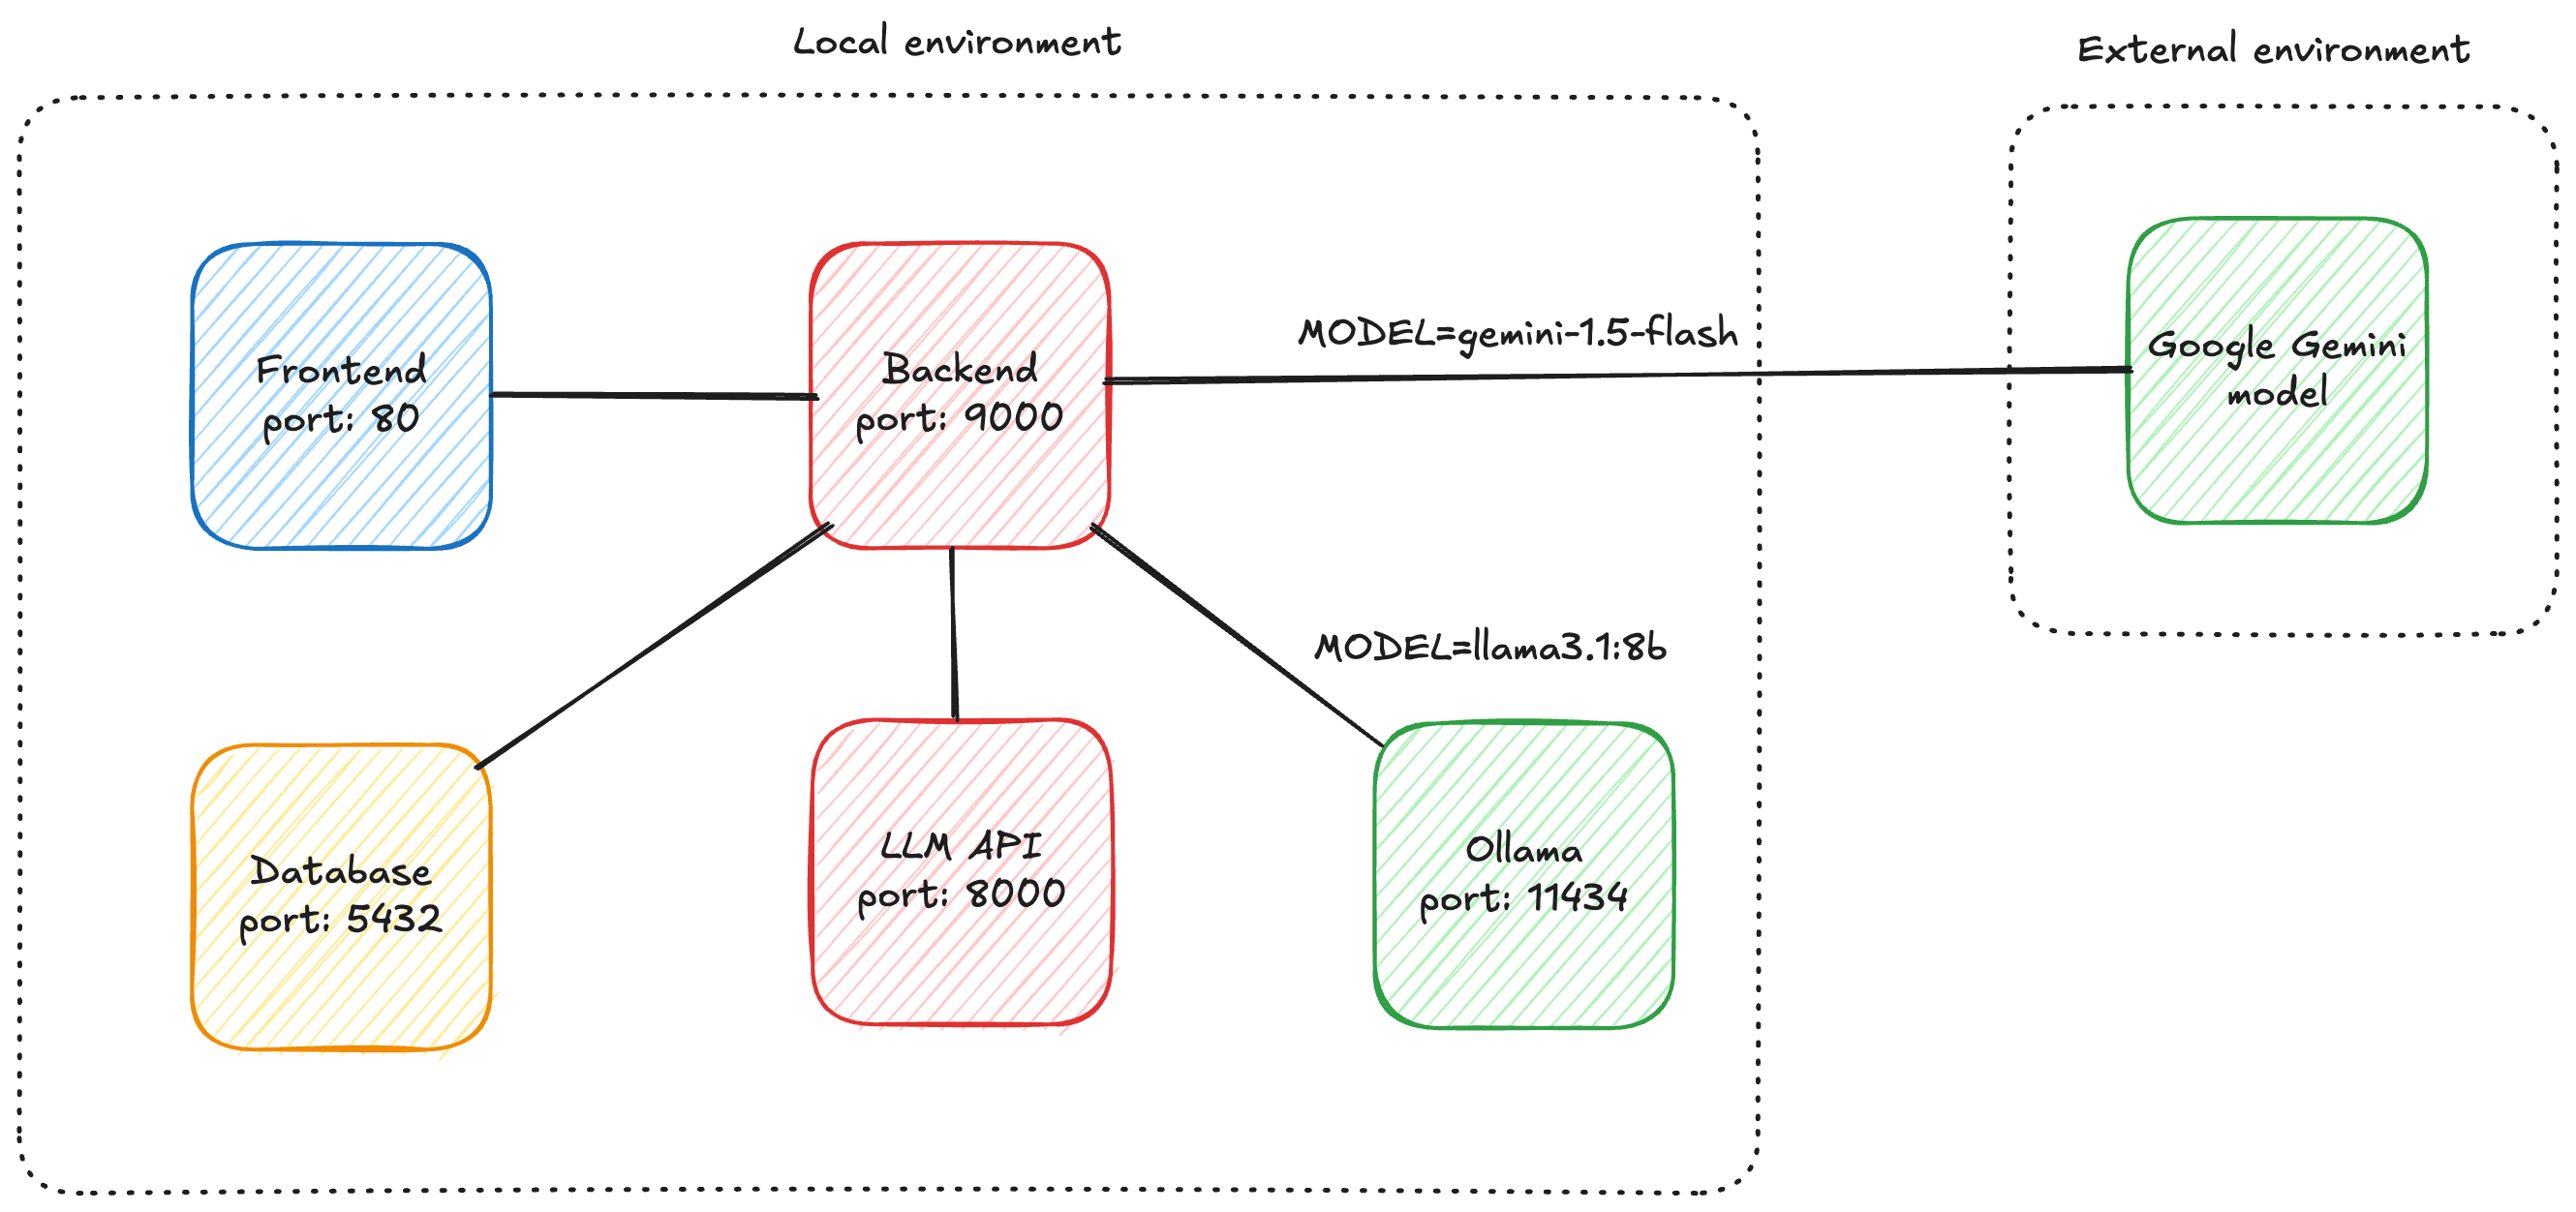
\includegraphics[width=0.8\textwidth, keepaspectratio]{figures/dev-deployment.png}
    \caption{Developer deployment}
    \label{fig:dev-deployment}
\end{figure}

\subsubsection{Production deployment}

We use a similar structure for production but without the Gemini model. We also split up the parts in this case into two, as Figure \ref{fig:production-deployment} shows. The regular services (frontend, backend, database, LLM API) are found on Máté's VPS (Virtual Private Server) in a Kubernetes\footnote{https://kubernetes.io/} cluster, while the AI model is deployed to an external provider. The VPS has no GPU; thus, we selected a provider specializing in running LLMs.

\begin{figure}[!h]
    \centering
    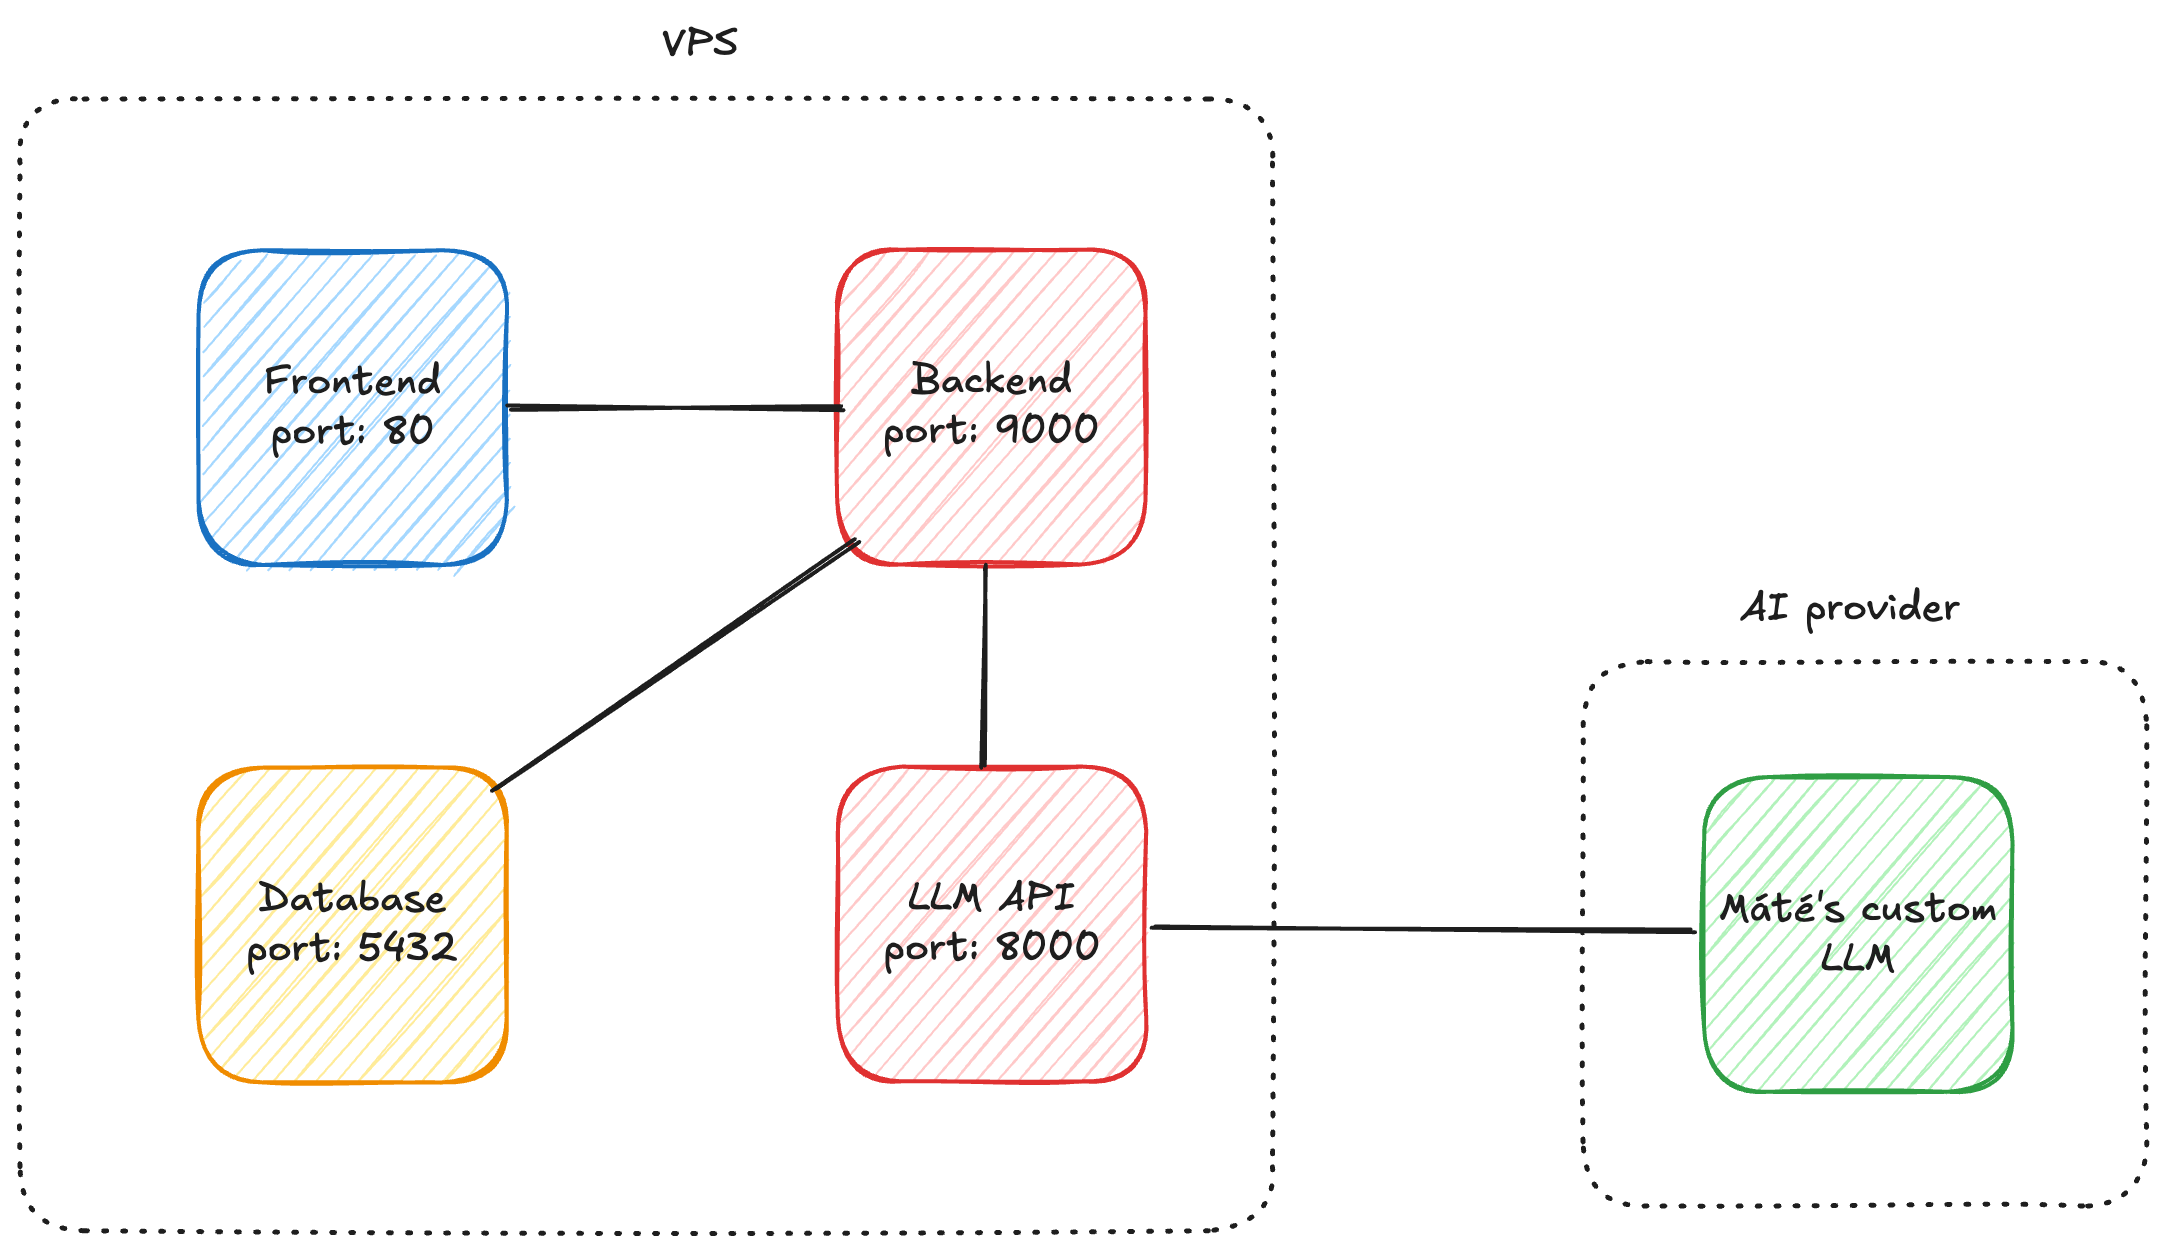
\includegraphics[width=0.8\textwidth, keepaspectratio]{figures/production-deployment.png}
    \caption{Production deployment}
    \label{fig:production-deployment}
\end{figure}

\section{Database Design}

Database design and software selection are critical parts of every web application; the same applies to the platform. Thus, we chose a relational database, Postgres, to store and serve the platform's data. I write about the database software selection and its rationale after introducing the data model from multiple aspects and the decisions behind them.

\subsection{Database software selection}

Postgres is one of the most popular Database Manager System (DBMS) software available today. It is free and open-source and offers a ready-to-use solution as a Docker container. We have worked with it for different projects through the years, and it has always been a good choice. So, its familiarity and reliability were the most important reasons for selecting it, besides its performance and wide adaption at database providers. 

Although it is a traditional database, it is extendable with third-party extensions. Its package manager is called trunk\footnote{https://pgt.dev/}, and it is effortless to install database packages by using it. We installed pgvector\footnote{https://github.com/pgvector/pgvector} for vector database features for the AI and another one called pgchron\footnote{https://github.com/citusdata/pg_cron} for scheduling session-related tasks.

\subsection{Entity-Relationship diagrams}

This section discusses the entities and their relationships in the application at this layer. I split it up into six smaller parts for easier understanding and overviewing.

\subsubsection{Users and sessions}

The database has two entities tightly connected to the user: User and Session. The User entity holds regular information about the user, like name, email, and hashed password, while the session stores the current user's session and its validity. When the user authenticates, a session is created and sent to the user's computer as a session cookie for later use. The session ID is used for authentication throughout the whole platform and has an expiration date when a pgchron task automatically deletes it. Figure \ref{fig:er-user-and-session} displays the entities and the relationship between them.

\begin{figure}[H]
    \centering
    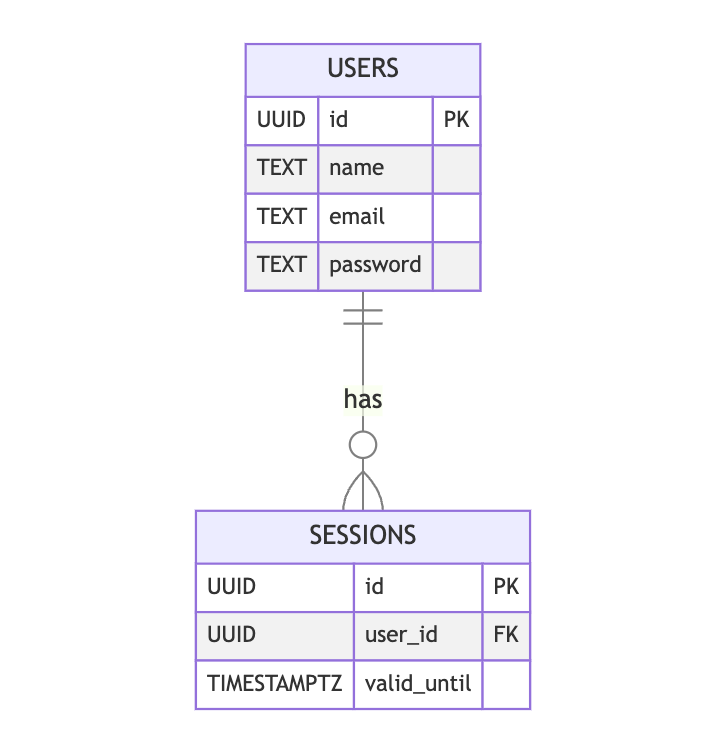
\includegraphics[width=0.8\textwidth, keepaspectratio]{figures/er-user-and-session.png}
    \caption{ER Diagram: User and Session}
    \label{fig:er-user-and-session}
\end{figure}

\subsubsection{Quizzes and questions}

The platform's core entities are the Quizzes and their questions. Each quiz has a name, description, and creator and is linked to different types of questions. There are three types of questions: SingleChoiceQuestion, a question with only one correct answer; MultipleChoiceQuestion, which can have multiple correct answers; and TrueOrFalseQuestion, aka a boolean question. Each type has its entity and table in the database. They are mostly the same; they all have a more extended text field describing the question and differ in the answer type.

The quizzes can be accessed through a QuizAccess entity, which links the user to a quiz with a role. By default, an instance with an owner role is generated automatically when a user creates a quiz. This abstraction allows controlling which quiz can be viewed or edited by whom. It also makes it available for future development as a platform for sharing private quizzes or creating public ones. Figure \ref{fig:er-quizzes} displays the quizzes, types of questions, and accesses in an ER diagram.

\begin{figure}[H]
    \centering
    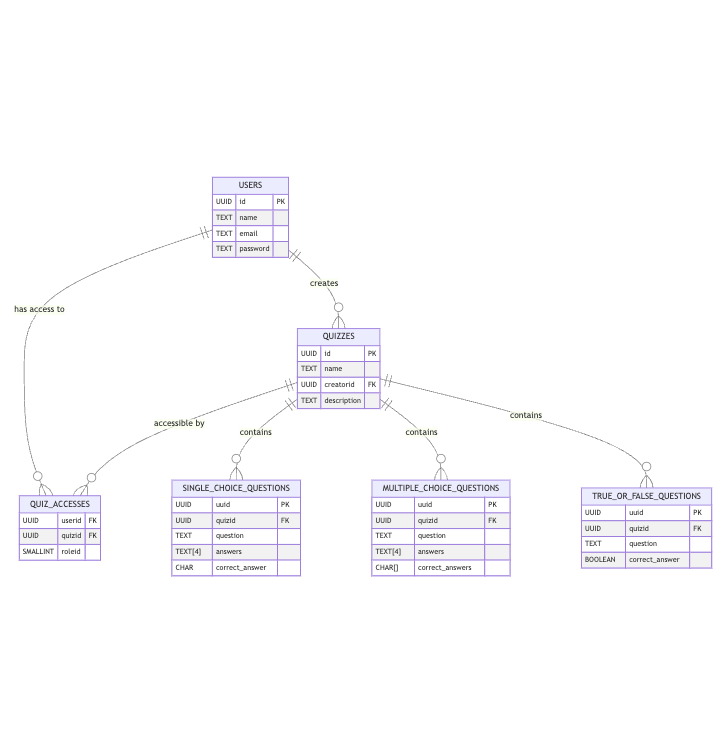
\includegraphics[width=0.8\textwidth, keepaspectratio]{figures/er-quizzes.png}
    \caption{ER Diagram for quizzes and questions}
    \label{fig:er-quizzes}
\end{figure}

\subsubsection{Quiz sessions}

Another essential entity category is related to answering questions. The central entity is the QuizSession, which holds the information together for quiz completion. It accounts for start and finish time and links to answers connected to questions. And it is also related to the quiz result if it is submitted. Some answer entities hold the information of the user's answer to the given question. Figure \ref{fig:er-quiz-session} shows these relations.

\begin{figure}[H]
    \centering
    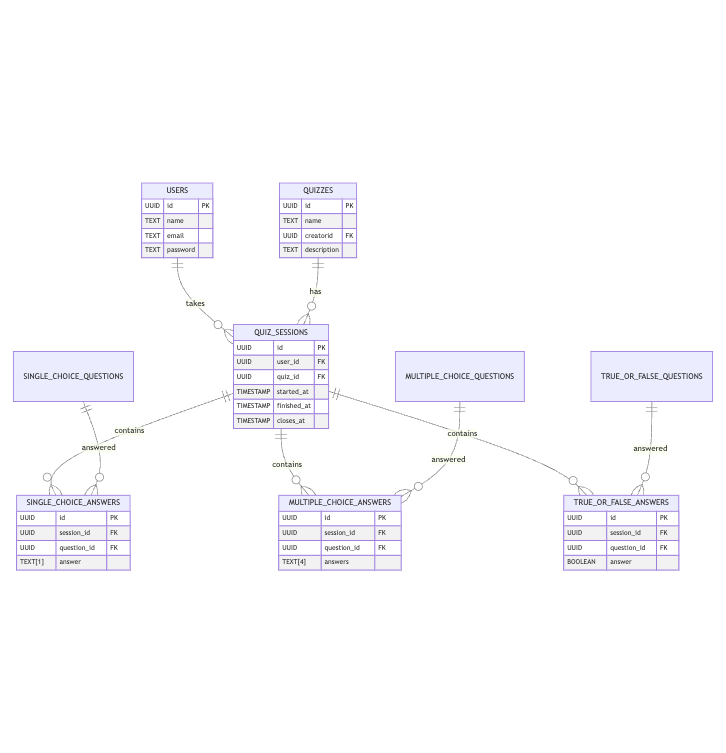
\includegraphics[width=0.8\textwidth, keepaspectratio]{figures/er-quiz-sessions.png}
    \caption{ER Diagram for quiz sessions}
    \label{fig:er-quiz-session}
\end{figure}

\subsubsection{Answers and quiz results}

In addition to the entities detailed before, there are more entities related to QuizSession, but now, it is for storing the scores for the answers and the results of the finished one. When a quiz is submitted and the session is finished, AnswerScore entities are created, which store the user's score for their given answers, and a question result record is also added with total scores. QuizResult is just a supporting entity for later extensibility capabilities; currently, it could have been merged into the QuizSession. 

\begin{figure}[H]
    \centering
    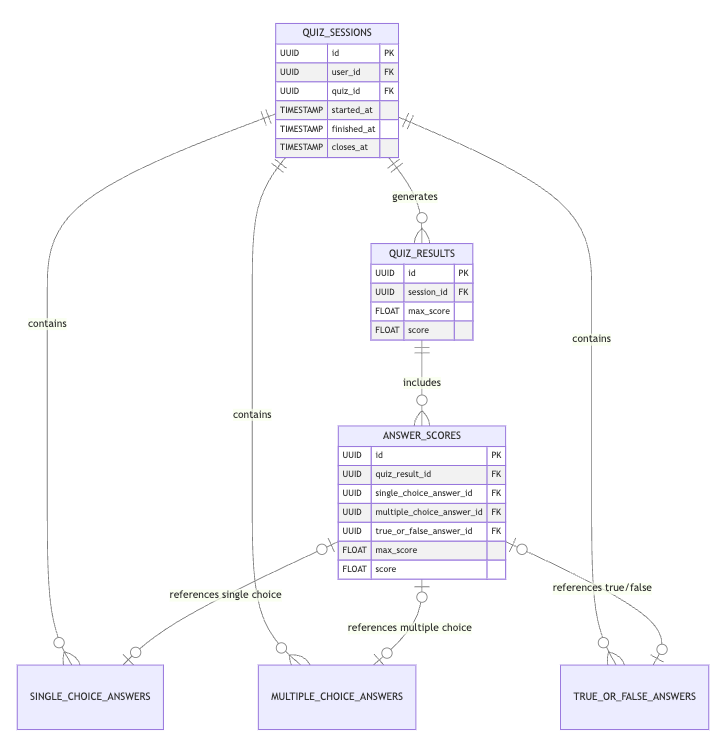
\includegraphics[width=0.8\textwidth, keepaspectratio]{figures/er-quiz-result.png}
    \caption{ER Diagram for answers and quiz results}
    \label{fig:er-quiz-result}
\end{figure}

Each AnswerScore has a max\_score and score field, which holds the maximum available and the obtained score. It establishes three distinct relationships corresponding to different question types. These relationships are structured with cardinality constraints, ensuring that a single AnswerScore can be linked to only one question at a time, maintaining a one-to-zero or one-to-one connection depending on the specific question type. Figure \ref{fig:er-quiz-result} shows all the entities and relations mentioned in these paragraphs.

\subsubsection{Learn list}

\begin{figure}[H]
    \centering
    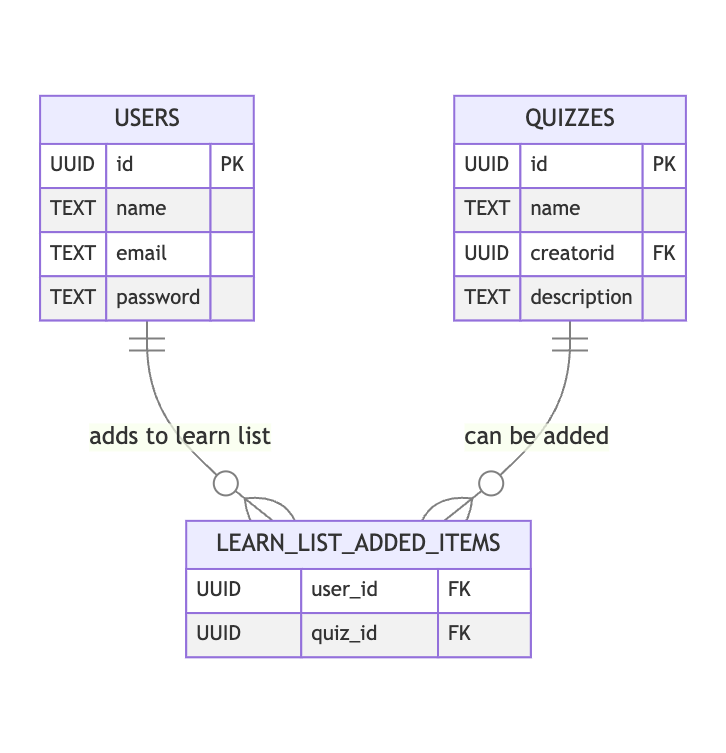
\includegraphics[width=0.8\textwidth, keepaspectratio]{figures/er-learn-list.png}
    \caption{ER Diagram for learn list}
    \label{fig:er-learn-list}
\end{figure}

\subsubsection{Review items}

\begin{figure}[H]
    \centering
    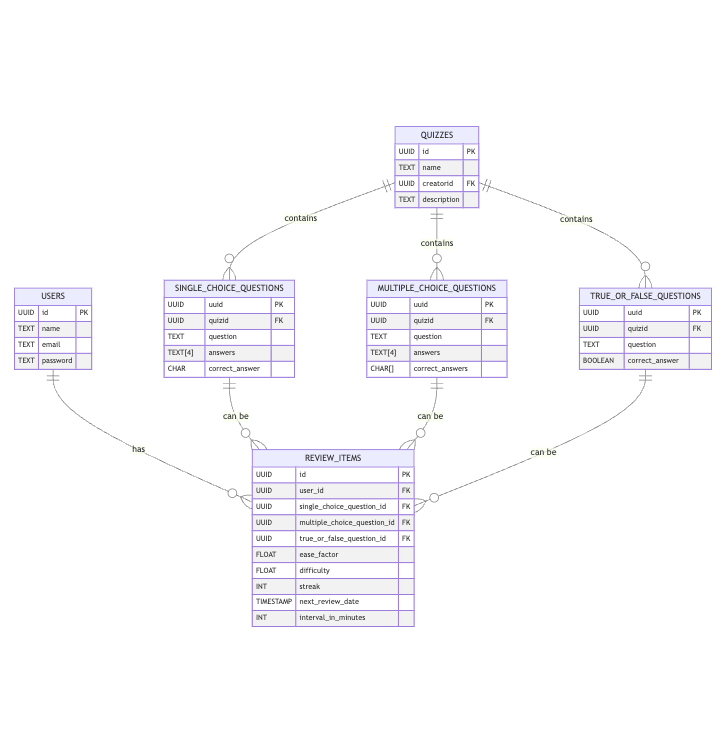
\includegraphics[width=0.8\textwidth, keepaspectratio]{figures/er-review-items.png}
    \caption{ER Diagram for review items}
    \label{fig:er-review items}
\end{figure}

\subsection{Database schema}

\subsection{Key tables and their relationships}

\subsubsection{Core tables}
    
\subsubsection{Supporting tables}
    
\subsection{Data modeling decisions}

\subsubsection{Indexing strategy}

\subsubsection{Data type selection}

\subsubsection{Constrains and integrity rules}

\section{Frontend Design}

\subsection{User Interface (UI) design principles}

\subsubsection{Chosen design metolodogy}

\subsubsection{User experience (UX) goals}

\subsubsection{Design system planning}

\subsection{Architecture Planning}

\subsubsection{Selected frontend architecture pattern and rationale}
        
I adopted a server-side-driven architecture using HTMX and Go for the application. It is a Multi-Page Architecture (MPA) at the core but leverages the framework's SPA-like capabilities. The architectural pattern consists of server-side HTML generation, HTMX enhancement, and the component structure.

The server generates the pages dynamically using the templating engine called templ. The dynamic content is served through partial HTML updates with HTMX requests. This way, the server controls the UI state instead of the client. The approach has several benefits: it decreases the initial site load and simplifies state management because the client receives the complete page containing the client state.

The HTMX library provides the interactions with its AJAX request boosting feature. Applications using the framework can act like single-page applications because the in-place content updates could replace full-page reloads. The approach offers progressive enhancement by not requiring rewriting everything initially and reduces writing additional JavaScript even to zero lines.

The UI is organized into reusable components. They are written in Go using templ.

\subsubsection{Component hierarchy planning}

\subsubsection{}

\section{Backend Design}

\section{AI integration Design}
\chapter{Implementation}

This chapter introduces some interesting implementation details and techniques, focusing mainly on the frontend but also mentioning the backend, including the spaced repetition algorithm.


\section{Frontend implementation}

This section presents the completed frontend application, illustrated with pictures, and then describes the solutions used during the implementation, highlighting the exciting features.

\subsection{The frontend application and screenshots}

TODO

\subsection{Project structure}

The project follows a flat folder structure hierarchy inspired by \texttt{The Go Standard Project Layout}\footnote{https://github.com/golang-standards/project-layout}. Figure \ref{fig:frontend-project-structure} shows this folder structure visually.

\begin{figure}[H]
    \centering
    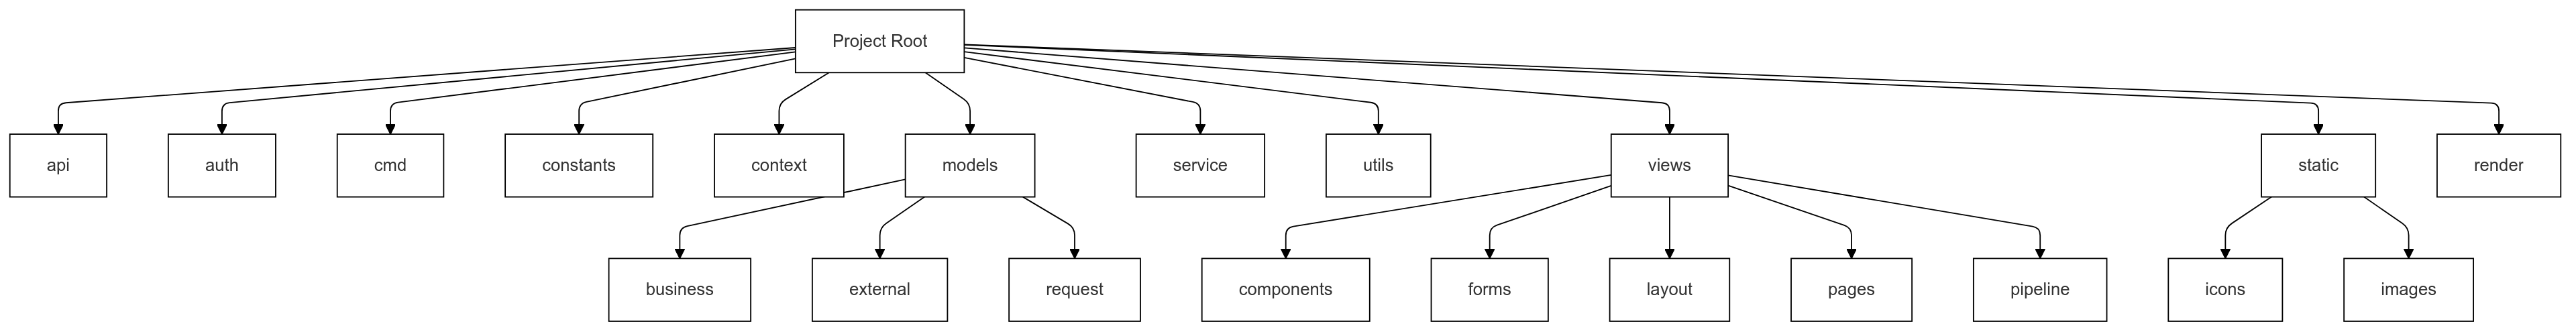
\includegraphics[width=0.8\textwidth, keepaspectratio]{figures/frontend-project-structure.png}
    \caption{Frontend project structure}
    \label{fig:frontend-project-structure}
\end{figure}

\textbf{api}: The \texttt{api} folder contains the endpoint handlers related to the pages and HTMX interactions.

\textbf{auth}: The \texttt{auth} folder contains the endpoint handlers related to the authentication function of the platform.

\textbf{cmd}: The folder \texttt{cmd} is a Go-specific folder containing the main functions. It is a common way to define the entry point of an application in \texttt{cmd/main.go}.

\textbf{constants}: The \texttt{constants} folder contains run-time constants; they wrap the provided environment variables and make them globally available for the application.

\textbf{context}: The \texttt{context} folder contains the custom context of the application. This context includes user information like a session ID and username.

\textbf{models}: The \texttt{models} folder contains Go representations of the data models in different layers and provides mappings between them. There are three layers of data: business, external, and request, which are separated into subfolders.

\textbf{service}: The \texttt{service} folder contains the ApiService, a proxy service providing access to the backend via function calls. This service is accessible through the custom context because the server calls usually require attaching the session ID to the request, and this service can do it automatically.

\textbf{utils}: The \texttt{utils} folder contains utils functions like generating gradient background from UUIDs and finding elements in lists.

\textbf{view}: The \texttt{view} folder contains the templ components and the generated Go code generated from them. They are also separated into subfolders based on their usage: \texttt{components}, \texttt{forms}, \texttt{layout}, \texttt{pages}, and \texttt{pipeline}.

\textbf{static}: The \texttt{static} folder is a regular webserver folder containing static resources for the application, such as scripts, images, and icons.

\textbf{render}: The \texttt{render} folder contains the configuration of the templ renderer and the render pipeline.

\subsection{Data models}

The application operates with three layers of data models. Each has a specific use case and can be mapped into other layer equivalents with mapping functions. These layers are the following: \texttt{business} used for doing the business logic, \texttt{external} used as Data Transfer Objects (DTO), and \texttt{request} used as communicating with the user. Listing \ref{lst:mapping-example} shows an example for mapping a quiz result object from \texttt{external} to \texttt{business} layer.

\begin{lstlisting}[caption=Mapping from external to business,label=lst:mapping-example]
func (result *QuizResult) MapToBusiness() (*business.QuizResult, error) {
    answerScores := make([]business.AnswerScore, 0, len(result.AnswerScores))
    for _, score := range result.AnswerScores {
        answerScore, err := score.MapToBusiness()
        if err != nil {
            return nil, err
        }
        answerScores = append(answerScores, *answerScore)
    }

    return &business.QuizResult{
        ID:           result.ID,
        SessionID:    result.SessionID,
        MaxScore:     result.MaxScore,
        Score:        result.Score,
        AnswerScores: answerScores,
    }, nil
}
\end{lstlisting}

The business layer objects are usually mappings from DTOs, with minor changes for effortless rendering. The DTOs are Go structs with \texttt{struct tags} used for parsing JSON objects. They are mostly the same as used on the backend. The request layer objects are similar to DTOs, but their \texttt{struct tags} help to map form data sent by the client instead of JSON sent by the server.

\subsection{Authentication}\label{subsec:frontend-authentication}

The authentication on the client side is an extension of the server-side version. The user sends the session cookie to the frontend, and the frontend server saves it in the execution context and uses it to fetch data from the backend. A custom context is created from the Echo context on each request by extending it with user-related information and instantiating an ApiService instance. The ApiService automatically attaches the session cookie to the requests before sending them to the backend. Listing~\ref{lst:session-middleware} shows the code of the custom session middleware.

\begin{lstlisting}[caption=Session middleware code,label=lst:session-middleware]
func SessionMiddleware(next echo.HandlerFunc) echo.HandlerFunc {
	return func(c echo.Context) error {
		cc := &AppContext{
			Context: c,
		}

		sessionCookie, err := c.Cookie("session")
		if err != nil {
			return next(cc)
		}

		cc.ApiService = service.NewApiService(sessionCookie)
		session, err := cc.ApiService.GetSession()
		if err != nil {
			return next(cc)
		}

		cc.Session = session
		cc.Set("cc", cc)
		return next(cc)
	}
}
\end{lstlisting}

The custom context creation and session checking are built on the Echo framework middleware feature. I defined a middleware that extends the Echo context and another that checks the extended context to contain the session information. The session creator middleware is placed before every request because it only tries extending the context, but the other one is placed before the execution of the authentication-required endpoint to ensure the user is authenticated. It works like the Angular web framework's Auth guard \footnote{https://angular.dev/api/router/CanActivate} feature. Listing \ref{lst:session-require-middleware} shows the middleware code that ensures the authentication.

\begin{lstlisting}[caption=Session checking middleware code,label=lst:session-require-middleware]
func RequireSessionMiddleware(next echo.HandlerFunc) echo.HandlerFunc {
	return func(c echo.Context) error {
		cc, ok := c.(*AppContext)
		if !ok || cc.Session == nil {
			return c.Redirect(http.StatusFound, "/login")
		}
		return next(c)
	}
}
\end{lstlisting}

\subsection{Rendering pipeline}

I designed a pipeline-like structure for rendering the components to make them easier to manage and use. The pipeline has three stages: two primary and one optional. These stages have different responsibilities and use cases, but they were a good addition to creating a well-organized render structure. The first stage determines the request type, the second renders the desired component(s), and the final extends the rendered component when necessary. The following figure~\ref{fig:rendering-pipeline} shows the whole rendering process.

\begin{figure}[H]
    \centering
    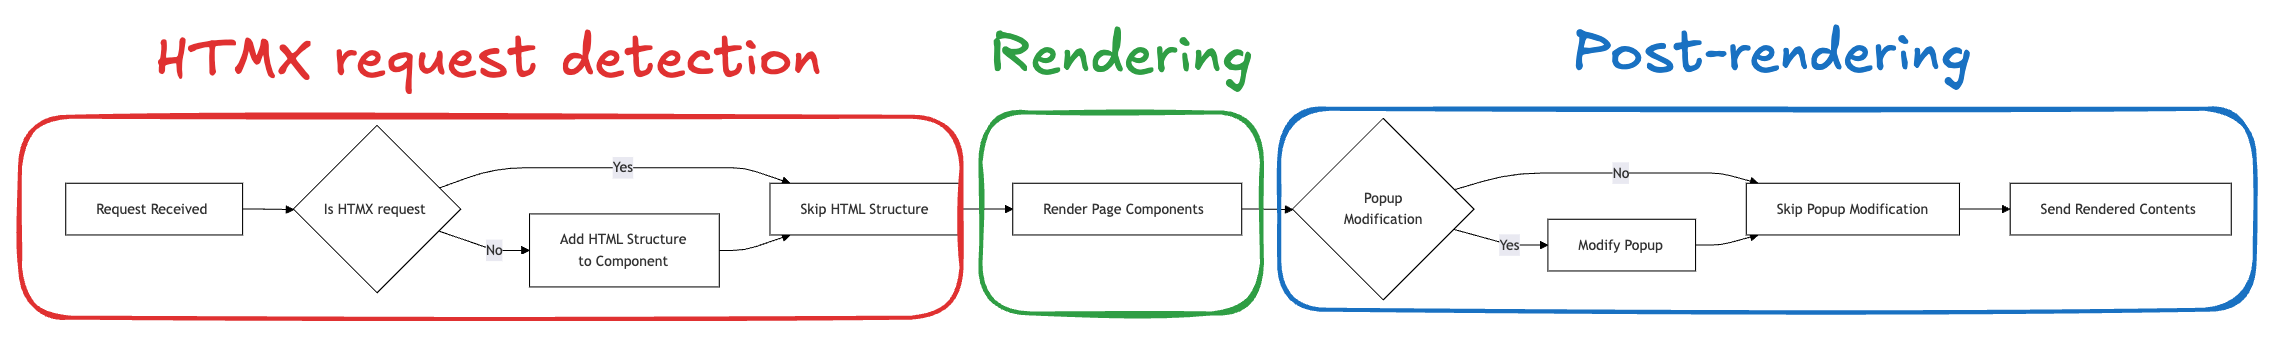
\includegraphics[width=0.8\textwidth, keepaspectratio]{figures/rendering-pipeline.png}
    \caption{Rendering pipeline}
    \label{fig:rendering-pipeline}
\end{figure}

The main problem was rendering the pages in a unified way for different needs. When a user navigates between pages, the frontend server should only render the page and the modified sidebar and let HTMX insert them into the DOM tree. However, when a user accesses a page directly with the URL, the server has to render a base HTML layout containing the scripts and styles in addition to the page and the sidebar—the pipeline's first stage checks whether the incoming request is a standard AJAX or an HTMX-boosted one.

The central stage of the pipeline is responsible for rendering the pages and components. It doesn't have to know whether a rendered element works as it is or is placed into a structure. This stage also allows additional components to be added, but it has to be done manually based on the use case. A common use case is using the HTMX OOB requests to update different parts of an application.

The final stage is responsible for automatically making post-render modifications. Currently, the only use case for this feature in the application is closing popups on navigation. It is made to be extendable, such as keeping a popup open, and can be set, but it has yet to be used.

\subsection{Form handling}

The HTMX requests contain information in HTTP forms. I used an interesting technique \footnote{https://www.youtube.com/watch?v=bQirFmhS3iw} for rendering and validating these forms in the application. The main idea is adding two parameters to the form components; the first is Go struct representing the values filled by the user, and the second is storing error messages. When a user submits a form, the frontend parses the values into the struct and validates them. If any error occurs or a value is inappropriate, the frontend server attaches error messages with keys to the error map and renders the component using the values and the messages. The following listing~\ref{lst:form-handling} shows the login form component's code and how the values and the error messages are set.

\begin{lstlisting}[caption=Login form,label=lst:form-handling]
templ LoginForm(errors map[string]string) {
	<form
		hx-post="/login"
		hx-swap="outerHTML"
		class="flex flex-col gap-y-4 p-6 w-[500px]"
	>
		<span class="text-center text-3xl font-bold">Login</span>
		@components.EMailInput(components.EMailInputProps{
			Error: errors["email"],
		})
		@components.TextInput(components.TextInputProps{
			Name:        "password",
			Label:       "Password",
			Placeholder: "Password",
			Type:        "password",
			Error:       errors["password"],
		})
		@components.Button(components.ButtonProps{
			Text: "Submit",
			Type: "submit",
		})
		@components.LinkButton("Sign up", "/signup", components.ButtonColorWhite)
		if errors["other"] != "" {
			<span class="w-full py-4 text-red-500 text-nowrap">{ errors["other"] }</span>
		}
	</form>
}
\end{lstlisting}

\subsection{Backend integration}

The frontend server makes HTTP requests to the backend endpoints using the ApiService from the context. ApiService is a proxy class that abstracts HTTP requests into function calls. It offers a unified and automated way to communicate with the backend. The session middleware constantly creates one instance for the current context containing the session information. The service's responsibility is to attach the session cookie to each request, and it manages by offering a common request sending and parsing function. This function takes the URL, HTTP method name, request, and response objects as parameters, creates a request, attaches the session cookie to the HTTP header, and processes the request. Listing \ref{lst:api-service} shows the code of this util function.

\begin{lstlisting}[caption=ApiService code,label=lst:api-service]
func (a *ApiService) getResponse(method, path string, requestBody any, responseBody interface{}) error {
	data, err := json.Marshal(requestBody)
	if err != nil {
		return err
	}

	req, err := http.NewRequest(method, constants.BACKEND_URL+path, bytes.NewBuffer(data))
	if err != nil {
		return err
	}

	if a.sessionCookie != nil {
		req.AddCookie(a.sessionCookie)
	}

	resp, err := a.client.Do(req)
	if err != nil {
		return err
	}
	defer resp.Body.Close()

	if resp.StatusCode >= 400 {
		bodyBytes, err := io.ReadAll(resp.Body)
		if err != nil {
			return err
		}

		var result map[string]string
		err = json.Unmarshal(bodyBytes, &result)
		if err != nil {
			return err
		}

		return errors.New("error message: " + result["message"])
	}

	err = json.NewDecoder(resp.Body).Decode(&responseBody)
	if err != nil {
		return err
	}

	return nil
}
\end{lstlisting}

\section{Backend implementation}

The backend server is a traditional API server that functions as the platform's core component. It is written in Go using the Echo web framework. This section details the project, how the data is used, and how the authentication, database communication, or the spaced repetition algorithm are implemented. This section focuses on highlighting the exciting and unique details of the implementation.

\subsection{Project structure}

The backend follows a flat folder structure hierarchy similar to the frontend with backend-specific features. This structure is a bit chaotic now, mainly due to using different SQL libraries. It needs some changes, but it is suitable for now. Figure~\ref{fig:backend-project-structure} shows the structure visually. Some parts, for example, config files, are missing from the figure because they are placed into the root, but this figure is about the folders.

\begin{figure}[H]
	\centering
	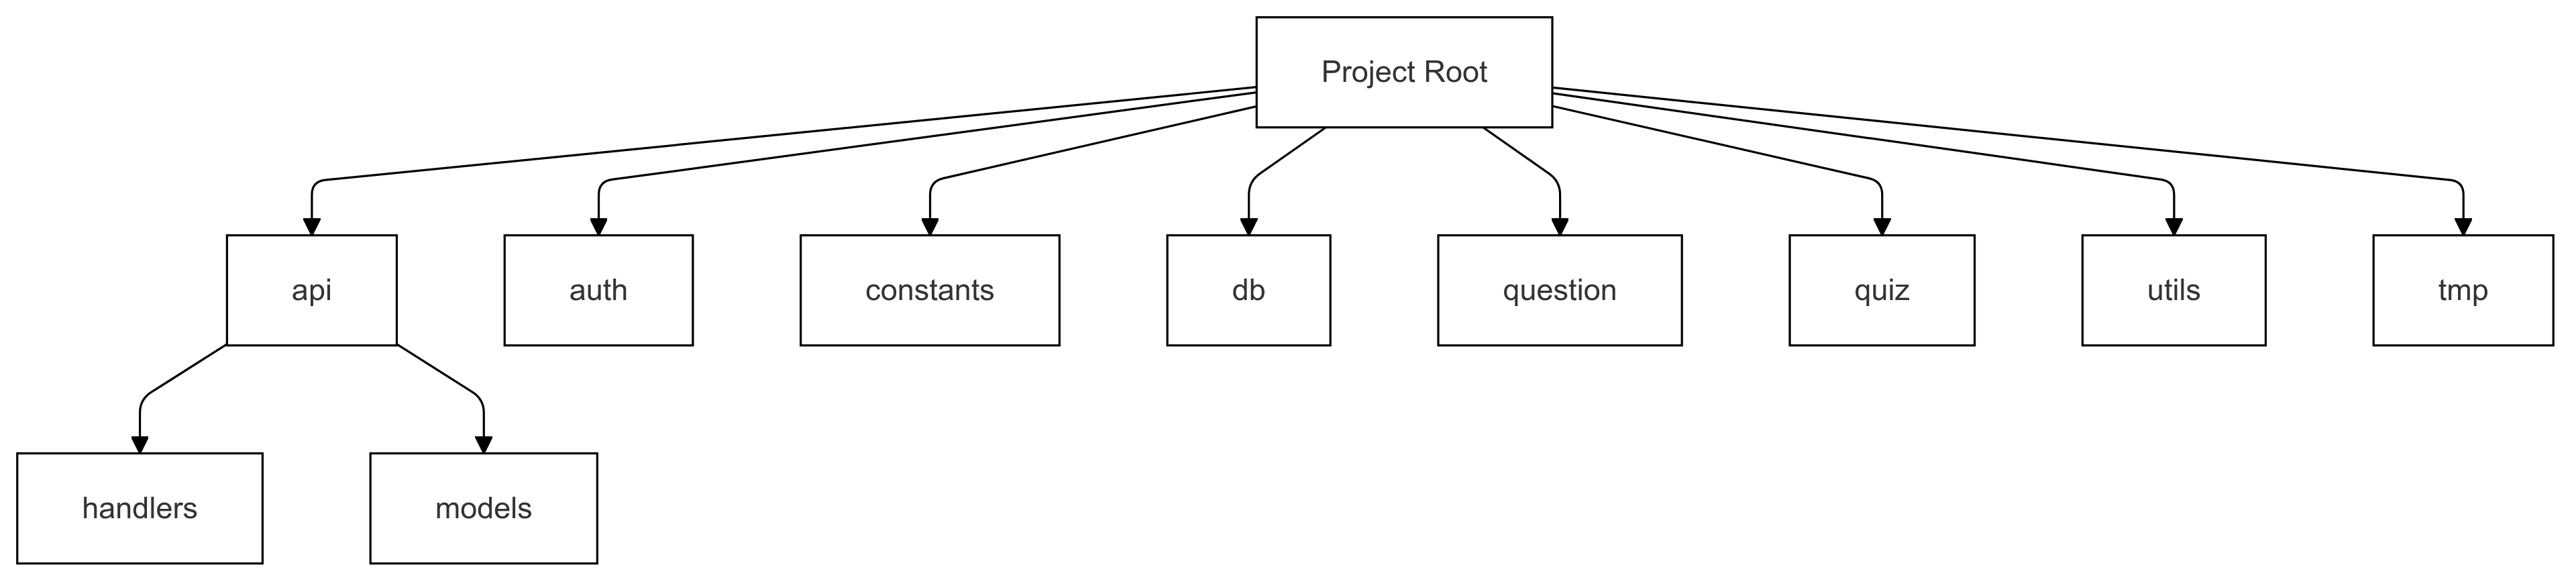
\includegraphics[width=0.8\textwidth, keepaspectratio]{figures/backend-project-structure.png}
	\caption{Backend project structure}
	\label{fig:backend-project-structure}
\end{figure}

\textbf{api}: The \texttt{api} folder contains the endpoint handlers and the DTO's. They are separated into two subfolders: \texttt{handlers} and \texttt{models}.

\textbf{auth}: The \texttt{auth} folder stores the authentication-related endpoint handlers, models, and database queries. These functions are placed here. They are implemented using the SQLx library.

\textbf{constants}: The \texttt{constants} folder is the same as in the fronted. It contains run-time constants and wraps environment variables into Go variables.

\textbf{db}: The \texttt{db} folder is a generated folder by SQLc, containing the SQL schemas, queries, and the glue code for accessing the database.

\textbf{question} and \textbf{quiz}: These two folders are for database codes and types used by the SQLx library, containing prepared statements and mapping types.

\textbf{utils}: The \texttt{utils} folder contains shared code for the application. Currently, they are database-related helper functions.

\textbf{tmp}: The \texttt{tmp} folder is a temporary folder containing the application's binary and related log files.

\subsection{Data models}

Unlike the frontend, backend data can be split into two layers: business and Data Access Object (DAO). In the case of the backend, the DTO and the business layer are merged. The business logic is performed on these objects containing the JSON parsing related \texttt{struct tags}. For now, it is sufficient, but I may need to separate them later.

The DAO layer contains the objects the database libraries use to map rows to the Go code. I do not apply them directly but map to their business layer equivalents to perform logic. There are two categories: the ones I wrote in Go for the SQLx library queries and the ones other SQL library generates. Listing~\ref{lst:sqlx-type} shows an example SQLx-compatible type struct declaration.

\begin{lstlisting}[caption=SQLx-compatible type struct declaration,label=lst:sqlx-type]
type DBSingleChoiceQuestion struct {
    UUID          string         `db:"uuid"`
    QuizID        string         `db:"quizid"`
    Question      string         `db:"question"`
    Answers       pq.StringArray `db:"answers"`
    CorrectAnswer string         `db:"correct_answer"`
}
\end{lstlisting}

\subsection{Authentication}

The platform uses session-based authentication with HTTP cookies. The frontend side of the implementation is discussed earlier in the frontend authentication subsection~\ref{subsec:frontend-authentication}. This subsection focuses on the backend side.

The implementation is straightforward; the service offers the endpoint \texttt{/authenticate-user}, where a user can submit the credentials, and the server creates a session. This session's ID is an HTTP cookie in the response and must be sent back by the client on every request. The session is currently stored in the database in the session table. It is automatically deleted after expiring due to the in-database chron job. Listing~\ref{lst:session-creation} shows the code for creating the session.

\begin{lstlisting}[caption=Session creation code,label=lst:session-creation]
func CreateSession(userId string) (string, error) {
	var id string
	err := utils.DB.Get(&id, "INSERT INTO sessions (id, user_id, valid_until) VALUES (gen_random_uuid(), $1, now() + interval '1 hour') RETURNING id", userId)
	if err != nil {
		return "", err
	}
	return id, nil
}
\end{lstlisting}

The server reads the session cookie and compares it to the value stored in the database to check the session. This check can be done automatically by a session-checking middleware or manually with Go code on the desired endpoints. When the user logs out, the server deletes its session from the database, preventing others from stealing it.

\subsection{SQLc implementation}

SQLc is the library for accessing the database with generated code from schemas and queries. The library generates the code from the given schema and query files using its configuration file. This file helps define the style of the generated code. Listing~\ref{lst:sqlc-config} shows the current config of the SQLc library.

\begin{lstlisting}[caption=SQLc configuration,label=lst:sqlc-config]
version: "2"
sql:
  - engine: "postgresql"
    queries: "query.sql"
    schema: "schema.sql"
    gen:
      go:
        package: "db"
        out: "db"
        sql_package: "pgx/v5"
        emit_result_struct_pointers: true
        emit_pointers_for_null_types: true
        overrides:
          - db_type: "uuid"
            nullable: false
            go_type:
              type: "string"
              pointer: false

          - db_type: "uuid"
            nullable: true
            go_type:
              type: "string"
              pointer: true

          - db_type: "pg_catalog.float8"
            nullable: false
            go_type: "float64"

          - db_type: "pg_catalog.float8"
            nullable: true
            go_type: "float64"

\end{lstlisting}

The library generates a \texttt{db.Quieries} object containing the generated function calling prepared statements. This object requires a database connection to work. I created a service called \texttt{SQLCQuerier} to link these to objects. This service is initiated in the main function before everything else and stored as a global object. This object is called everywhere in the application to perform database queries. Every query function requires a go context and query-related parameter struct for the inner prepared statement. The context is used to limit the lifetime of the query execution. It helps prevent infinity loads and memory leaks. The following listing~\ref{lst:sqlc-querier} shows an example of retrieving the SQLCQuerier object and performing a request using it.

\begin{lstlisting}[caption=Using the SQLCQuerier,label=lst:sqlc-querier]
	// Get the querier and create a Go context with lifetime of 5s
	sqlcQuerier := utils.GetQuerier()
	ctx, cancel := context.WithTimeout(context.Background(), 5*time.Second)
	defer cancel()

	// Get sessions from the database using the querier
	quizSessions, err := sqlcQuerier.GetQuizSessionsByUserId(ctx, userID)
	if err != nil {
		return echo.NewHTTPError(http.StatusInternalServerError, fmt.Errorf("error getting quiz sessions for user: %w", err))
	}
\end{lstlisting}

\subsection{Spaced repetition algorithm}

The spaced repetition learning algorithm schedules the user's learning materials. It uses historical data gathered and stored in question-answering. When a user adds a quiz to its learning list, the platform finds the questions from the quiz and creates an immediate schedule with default values. It makes available the platform to check the user's answers and reschedule the questions based on the concrete answers.

The algorithm's implementation is straightforward; it consists of one function and a few lines of code. The functions take a review item and a score percentage as parameters and return the review item with the scheduled values. The review item represents a card used in the spaced repetition, and the score percentage is the score they got for the given question. The algorithm scales up the score between 1 and 5 for later calculations. Then, the score is higher than 3, meaning the user answered correctly with difficulties, or below it, meaning the answer needs to be corrected. Then, the algorithm calculates the difficulty, the ease factor, and the new schedule for the question. Finally, it stores the modified item and shows it to the user. Listing~\ref{lst:spaced-repetition} shows the concrete implementation of the algorithm written in Go.

\begin{lstlisting}[caption=Spaced repetition algorithm written in Go,label=lst:spaced-repetition]
func applySpacedRepetitionAndStore(ctx context.Context, reviewItem *models.ReviewItem, percentage float64) (*models.ReviewItem, error) {
	// score is the user's performance rating, where:
	// 5 = perfect recall, 4 = correct with minor hesitation, 3 = correct but difficult,
	// 2 = incorrect, but partially remembered, 1 = completely incorrect
	score := 5 * percentage

	if score >= 3 {
		reviewItem.Difficulty = math.Max(1, reviewItem.Difficulty-1)

		if reviewItem.Streak == 0 {
			reviewItem.IntervalInMinutes = 60
		} else if reviewItem.Streak == 1 {
			reviewItem.IntervalInMinutes = 3 * 60
		} else {
			reviewItem.IntervalInMinutes = int32(float64(reviewItem.IntervalInMinutes) * reviewItem.EaseFactor * (1 / reviewItem.Difficulty))
		}

		reviewItem.EaseFactor = reviewItem.EaseFactor + (0.1 - (5-score)*0.08)
		reviewItem.Streak = reviewItem.Streak + 1
	} else {
		reviewItem.Difficulty = math.Min(5, reviewItem.Difficulty+1.5)

		reviewItem.IntervalInMinutes = 60

		reviewItem.EaseFactor = math.Max(1.3, reviewItem.EaseFactor-0.2)
		reviewItem.Streak = 0
	}

	reviewItem.NextReviewDate = models.NullableTime{
		Time: reviewItem.NextReviewDate.Time.Add(time.Duration(reviewItem.IntervalInMinutes) * time.Minute),
	}

	// store the data ...

	return reviewItem, nil
}
\end{lstlisting}

\subsection{AI integration}

The AI features are found in different services but are available from the backend. They generate questions of a given type from the user-provided context. This context is usually several paragraphs long, so the server needs to split it into smaller parts. It not only speeds up the generation but also makes it more controllable. Máté made a simple algorithm for splitting up the context and iterating between the parts with a round-robin algorithm.

When a user submits long text as a question context, the server calculates a hash for later identification and splits it recursively into 2-3 paragraph chunks. For the first time, the first chunk and the question type are sent to the LLM API, which takes care of the generation. Next time, the server will check the hash and find the next chunk for the generation. These chunks are stored in the database and cached in memory to optimize retrieval speed.

The questions return from the LLM API as JSON objects in HTTP responses. The generation usually takes several seconds to finish; until then, the server and client have to wait. As I wrote this thesis, Máté and I started considering implementing HTTP streams besides the current method, allowing the client to show partially generated questions. This concept is more complicated than the implemented one and would need changes in every layer. It idea could be an excellent idea for improving the overall user experience.
\chapter{Conclusion and future work}\label{ch:conclusion-and-future-work}

%%----------------------------------------------------------------------------
\chapter{\LaTeX-eszközök}
\label{sec:LatexTools}
%----------------------------------------------------------------------------
\section{A szerkesztéshez használatos eszközök}
%----------------------------------------------------------------------------
Ez a sablon TeXstudio 2.8.8 szerkesztővel készült. A TeXstudio egy platformfüggetlen, Windows, Linux és Mac OS alatt is elérhető \LaTeX-szerkesztőprogram számtalan hasznos szolgáltatással (\refstruc{fig:TeXstudio}). A szoftver ingyenesen letölthető\footnote{A TeXstudio hivatalos oldala: \url{http://texstudio.sourceforge.net/}}.

\begin{figure}[!ht]
\centering
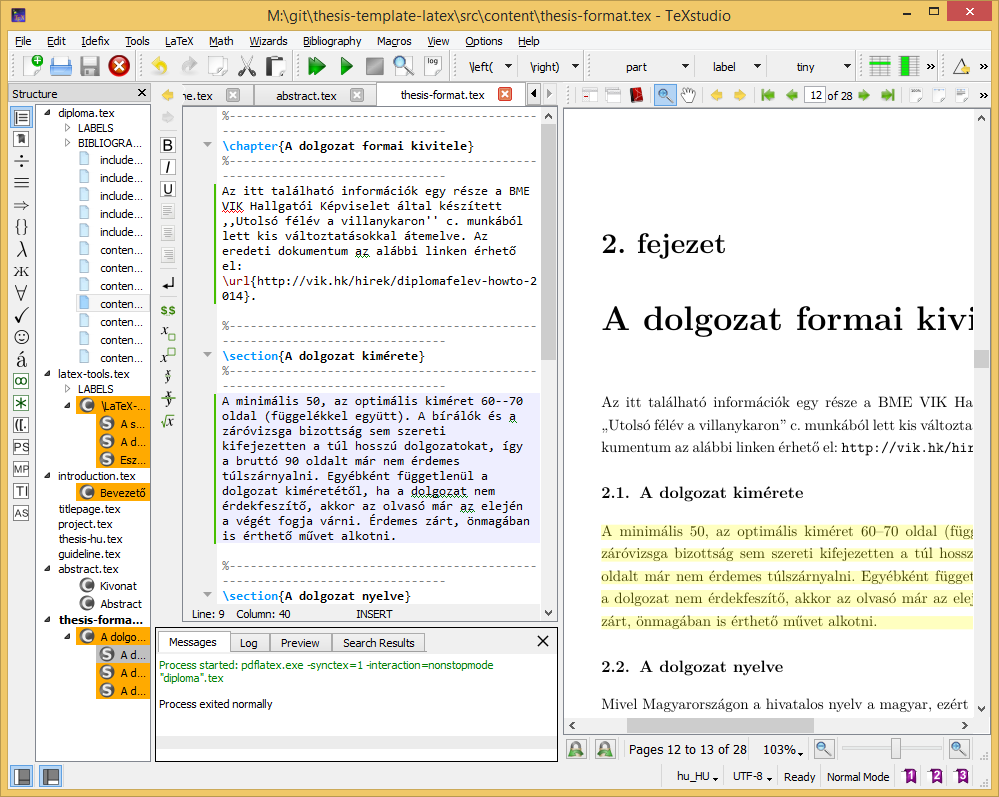
\includegraphics[width=150mm, keepaspectratio]{figures/TeXstudio.png}
\caption{A TeXstudio \LaTeX-szerkesztő.}
\label{fig:TeXstudio}
\end{figure}

A TeXstudio telepítése után érdemes még letölteni a magyar nyelvű helyesírásellenőrző-szótárakat hozzá. A TeXstudio az OpenOffice-hoz használatos formátumot tudja kezelni. A TeXstudio beállításainál a \verb+General+ fülön a \verb+Dictionaries+ résznél tudjuk megadni, hogy melyik szótárat használja.

Egy másik használható Windows alapú szerkesztőprogram a LEd\footnote{A LEd hivatalos oldala: \url{http://www.latexeditor.org/}} (LaTeX Editor), a TeXstudio azonban stabilabb, gyorsabb, és jobban használható.

%----------------------------------------------------------------------------
\section{A dokumentum lefordítása Windows alatt}
%----------------------------------------------------------------------------
A TeXstudio és a LEd kizárólag szerkesztőprogram (bár az utóbbiban DVI-nézegető is van), így a dokumentum fordításához szükséges eszközöket nem tartalmazza. Windows alatt alapvetően két lehetőség közül érdemes választani: MiKTeX (\url{http://miktex.org/}) és TeX Live (\url{http://www.tug.org/texlive/}) programcsomag. Az utóbbi működik Mac OS X, GNU/Linux alatt és Unix-származékokon is. A MiKTeX egy alapcsomag telepítése után mindig letölti a használt funkciókhoz szükséges, de lokálisan hiányzó \TeX-csomagokat, míg a TeX Live DVD ISO verzóban férhető hozzá. Ez a dokumentum TeX Live 2008 programcsomag segítségével fordult, amelynek DVD ISO verziója a megadott oldalról letölthető. A sablon lefordításához a disztribúcióban szereplő \verb+magyar.ldf+ fájlt a \verb+http://www.math.bme.hu/latex/+ változatra kell cserélni, vagy az utóbbi változatot be kell másolni a projekt-könyvtárba (ahogy ezt meg is tettük a sablonban) különben anomáliák tapasztalhatók a dokumentumban (pl. az ábra- és táblázat-aláírások formátuma nem a beállított lesz, vagy bizonyos oldalakon megjelenik alapértelmezésben egy fejléc). A TeX Live 2008-at még nem kell külön telepíteni a gépre, elegendő DVD-ről (vagy az ISO fájlból közvetlenül, pl. DaemonTools-szal) használni.

Ha a MiKTeX csomagot használjuk, akkor parancssorból a következő módon tudjuk újrafordítani a teljes dokumentumot:

\begin{lstlisting}[language=bash,frame=single,float=!ht]
$ texify -p thesis.tex
\end{lstlisting}

A \verb+texify+ parancs a MiKTex programcsomag \verb+miktex/bin+ alkönyvtárában található. A parancs gondoskodik arról, hogy a szükséges lépéseket (fordítás, hivatkozások generálása stb.) a megfelelő sorrendben elvégezze. A \verb+-p+ kapcsoló hatására PDF-et generál. A fordítást és az ideiglenes fájlok törlését elvégezhetjük a sablonhoz mellékelt \verb+manual_build.bat+ szkript segítségével is.

A \TeX-eszközöket tartalmazó programcsomag binárisainak elérési útját gyakran be kell állítani a szerkesztőprogramban, például TeXstudio esetén legegyszerűbben az \verb+Options / Configure TeXstudio... / Commands+ menüponttal előhívott dialógusablakban tehetjük ezt meg.

A PDF-\LaTeX~használata esetén a generált dokumentum közvetlenül PDF-formátumban áll rendelkezésre. Amennyiben a PDF-fájl egy PDF-nézőben (pl. Adobe Acrobat Reader vagy Foxit PDF Reader) meg van nyitva, akkor a fájlleírót a PDF-néző program tipikusan lefoglalja. Ilyen esetben a dokumentum újrafordítása hibaüzenettel kilép. Ha bezárjuk és újra megnyitjuk a PDF dokumentumot, akkor pedig a PDF-nézők többsége az első oldalon nyitja meg a dokumentumot, nem a legutóbb olvasott oldalon. Ezzel szemben például az egyszerű és ingyenes \textcolor{blue}{Sumatra PDF} nevű program képes arra, hogy a megnyitott dokumentum megváltozását detektálja, és frissítse a nézetet az aktuális oldal megtartásával.

%----------------------------------------------------------------------------
\section{Eszközök Linuxhoz}
%----------------------------------------------------------------------------
Linux operációs rendszer alatt is rengeteg szerkesztőprogram van, pl. a KDE alapú Kile jól használható. Ez ingyenesen letölthető, vagy éppenséggel az adott Linux-disztribúció eleve tartalmazza, ahogyan a dokumentum fordításához szükséges csomagokat is. Az Ubuntu Linux disztribúciók alatt például legtöbbször a \verb+texlive-*+ csomagok telepítésével használhatók a \LaTeX-eszközök. A jelen sablon fordításához szükséges csomagok (kb. 0,5 GB) az alábbi paranccsal telepíthetők:

\begin{lstlisting}[language=bash,morekeywords={sudo,apt\-get},alsoletter={-},breaklines=true]
$ sudo apt-get install texlive-latex-extra texlive-fonts-extra texlive-fonts-recommended texlive-xetex texlive-science
\end{lstlisting}

Amennyiben egy újabb csomag hozzáadása után hiányzó fájlra utaló hibát kapunk a fordítótól, telepítenünk kell az azt tartalmazó TeX Live csomagot. Ha pl. a \verb+bibentry+ csomagot szeretnénk használni, futtassuk az alábbi parancsot:

\begin{lstlisting}[language=bash,morekeywords={apt\-cache},alsoletter={-},breaklines=true]
$ apt-cache search bibentry
texlive-luatex - TeX Live: LuaTeX packages
\end{lstlisting}

Majd telepítsük fel a megfelelő TeX Live csomagot, jelen esetben a `texlive-lualatex`-et. (Egy LaTeX csomag több TeX Live csomagban is szerepelhet.)

Ha gyakran szerkesztünk más \LaTeX dokumentumokat is, kényelmes és biztos megoldás a teljes TeX Live disztribúció telepítése, ez azonban kb. 4 GB helyet igényel.

\begin{lstlisting}[language=bash,morekeywords={sudo,apt\-get},alsoletter={-},breaklines=true]
sudo apt-get install texlive-full
\end{lstlisting}

%%----------------------------------------------------------------------------
\chapter{A dolgozat formai kivitele}
%----------------------------------------------------------------------------
Az itt található információk egy része a BME VIK Hallgatói Képviselet által készített ,,Utolsó félév a villanykaron'' c. munkából lett kis változtatásokkal átemelve. Az eredeti dokumentum az alábbi linken érhető el: \url{http://vik.hk/hirek/diplomafelev-howto-2015}.

%----------------------------------------------------------------------------
\section{A dolgozat kimérete}
%----------------------------------------------------------------------------
Szakdolgozat esetében minimum 30, 45 körüli ajánlott oldalszám lehet az iránymutató. De mindenképp érdemes rákérdezni a konzulensnél is az elvárásokra, mert tanszékenként változóak lehetnek az elvárások.

Mesterképzésen a Diplomatervezés 1 esetében a beszámoló még inkább az Önálló laboratóriumi beszámolókhoz hasonlít, tanszékenként eltérő formai követelményekkel, -- egy legalább 30 oldal körüli dolgozat az elvárt -- és az elmúlt fél éves munkáról szól. De egyben célszerű, ha ez a végleges diplomaterv alapja is. (A végleges 60-90 oldal körülbelül a hasznos részre nézve)


%----------------------------------------------------------------------------
\section{A dolgozat nyelve}
%----------------------------------------------------------------------------
Mivel Magyarországon a hivatalos nyelv a magyar, ezért alapértelmezésben magyarul kell megírni a dolgozatot. Aki külföldi posztgraduális képzésben akar részt venni, nemzetközi szintű tudományos kutatást szeretne végezni, vagy multinacionális cégnél akar elhelyezkedni, annak célszerű angolul megírnia diplomadolgozatát. Mielőtt a hallgató az angol nyelvű verzió mellett dönt, erősen ajánlott mérlegelni, hogy ez mennyi többletmunkát fog a hallgatónak jelenteni fogalmazás és nyelvhelyesség terén, valamint -- nem utolsó sorban -- hogy ez mennyi többletmunkát fog jelenteni a konzulens illetve bíráló számára. Egy nehezen olvasható, netalán érthetetlen szöveg teher minden játékos számára.

%----------------------------------------------------------------------------
\section{A dokumentum nyomdatechnikai kivitele}
%----------------------------------------------------------------------------
A dolgozatot A4-es fehér lapra nyomtatva, 2,5 centiméteres margóval (+1~cm kötésbeni), 11--12 pontos betűmérettel, talpas betűtípussal és másfeles sorközzel célszerű elkészíteni.

Annak érdekében, hogy a dolgozat külsőleg is igényes munka benyomását keltse, érdemes figyelni az alapvető tipográfiai szabályok betartására~\cite{Jeney}.

%% !TeX spellcheck = hu_HU
% !TeX encoding = UTF-8
% !TeX program = xelatex
%----------------------------------------------------------------------------
\chapter{A \LaTeX-sablon használata}
%----------------------------------------------------------------------------

Ebben a fejezetben röviden, implicit módon bemutatjuk a sablon használatának módját, ami azt jelenti, hogy sablon használata ennek a dokumentumnak a forráskódját tanulmányozva válik teljesen világossá. Amennyiben a szoftver-keretrendszer telepítve van, a sablon alkalmazása és a dolgozat szerkesztése \LaTeX-ben a sablon segítségével tapasztalataink szerint jóval hatékonyabb, mint egy WYSWYG (\emph{What You See is What You Get}) típusú szövegszerkesztő esetén (pl. Microsoft Word, OpenOffice).

%----------------------------------------------------------------------------
\section{Címkék és hivatkozások}
%----------------------------------------------------------------------------
A \LaTeX~dokumentumban címkéket (\verb+\label+) rendelhetünk ábrákhoz, táblázatokhoz, fejezetekhez, listákhoz, képletekhez stb. Ezekre a dokumentum bármely részében hivatkozhatunk, a hivatkozások automatikusan feloldásra kerülnek.

A sablonban makrókat definiáltunk a hivatkozások megkönnyítéséhez. Ennek megfelelően minden ábra (\emph{figure}) címkéje \verb+fig:+ kulcsszóval kezdődik, míg minden táblázat (\emph{table}), képlet (\emph{equation}), fejezet (\emph{section}) és lista (\emph{listing}) rendre a \verb+tab:+, \verb+eq:+, \verb+sec:+ és \verb+lst:+ kulcsszóval kezdődik, és a kulcsszavak után tetszőlegesen választott címke használható. Ha ezt a konvenciót betartjuk, akkor az előbbi objektumok számára rendre a \verb+\figref+, \verb+\tabref+, \verb+\eqref+, \verb+\sectref+ és \verb+\listref+ makrókkal hivatkozhatunk. A makrók paramétere a címke, amelyre hivatkozunk (a kulcsszó nélkül). Az összes említett hivatkozástípus, beleértve az \verb+\url+ kulcsszóval bevezetett web-hivatkozásokat is a  \verb+hyperref+\footnote{Segítségével a dokumentumban megjelenő hivatkozások nem csak dinamikussá válnak, de színezhetők is, bővebbet erről a csomag dokumentációjában találunk. Ez egyúttal egy példa lábjegyzet írására.} csomagnak köszönhetően aktívak a legtöbb PDF-nézegetőben, rájuk kattintva a dokumentum megfelelő oldalára ugrik a PDF-néző vagy a megfelelő linket megnyitja az alapértelmezett böngészővel. A \verb+hyperref+ csomag a kimeneti PDF-dokumentumba könyvjelzőket is készít a tartalomjegyzékből. Ez egy szintén aktív tartalomjegyzék, amelynek elemeire kattintva a nézegető behozza a kiválasztott fejezetet.

%----------------------------------------------------------------------------
\section{Ábrák és táblázatok}
%----------------------------------------------------------------------------
Használjunk vektorgrafikus ábrákat, ha van rá módunk. PDFLaTeX használata esetén PDF formátumú ábrákat lehet beilleszteni könnyen, az EPS (PostScript) vektorgrafikus képformátum beillesztését a PDFLaTeX közvetlenül nem támogatja (de lehet konvertálni, lásd később). Ha vektorgrafikus formában nem áll rendelkezésünkre az ábra, akkor a  veszteségmentes PNG, valamint a veszteséges JPEG formátumban érdemes elmenteni.  Figyeljünk arra, hogy ilyenkor a képek felbontása elég nagy legyen ahhoz, hogy nyomtatásban is megfelelő minőséget nyújtson (legalább 300 dpi javasolt). A dokumentumban felhasznált képfájlokat a dokumentum forrása mellett érdemes tartani, archiválni, mivel ezek hiányában a dokumentum nem fordul újra. Ha lehet, a vektorgrafikus képeket vektorgrafikus formátumban is érdemes elmenteni az újrafelhasználhatóság (az átszerkeszthetőség) érdekében.

Kapcsolási rajzok legtöbbször kimásolhatók egy vektorgrafikus programba (pl. CorelDraw) és onnan nagyobb felbontással raszterizálva kimenthatők PNG formátumban. Ugyanakkor kiváló ábrák készíthetők Microsoft Visio vagy hasonló program használatával is: Visio-ból az ábrák közvetlenül PDF-be is menthetők.

Lehetőségeink Matlab ábrák esetén:
\begin{itemize}
	\item Képernyőlopás (\emph{screenshot}) is elfogadható minőségű lehet a dokumentumban, de általában jobb felbontást is el lehet érni más módszerrel.
	\item A Matlab ábrát a \verb+File/Save As+ opcióval lementhetjük PNG formátumban (ugyanaz itt is érvényes, mint korábban, ezért nem javasoljuk).
	\item A Matlab ábrát az \verb+Edit/Copy figure+ opcióval kimásolhatjuk egy vektorgrafikus programba is és onnan nagyobb felbontással raszterizálva kimenthatjük PNG formátumban (nem javasolt).
	\item Javasolt megoldás: az ábrát a \verb+File/Save As+ opcióval EPS \emph{vektorgrafikus} formátumban elmentjük, PDF-be konvertálva beillesztjük a dolgozatba.
\end{itemize}
Az EPS kép az \verb+epstopdf+ programmal\footnote{a korábban említett \LaTeX-disztribúciókban megtalálható} konvertálható PDF formátumba. Célszerű egy batch-fájlt készíteni az összes EPS ábra lefordítására az alábbi módon (ez Windows alatt működik).
\begin{lstlisting}[language=]
@echo off
for %%j in (*.eps) do (
  echo converting file "%%j"
  epstopdf "%%j"
)
echo done .
\end{lstlisting}

Egy ilyen parancsfájlt (\verb+convert.cmd+) elhelyeztük a sablon \verb+figures\eps+ könyvtárába, így a felhasználónak csak annyi a dolga, hogy a \verb+figures\eps+ könyvtárba kimenti az EPS formátumú vektorgrafikus képet, majd lefuttatja a \verb+convert.cmd+ parancsfájlt, ami PDF-be konvertálja az EPS fájlt.

Ezek után a PDF-ábrát ugyanúgy lehet a dokumentumba beilleszteni, mint a PNG-t vagy a JPEG-et. A megoldás előnye, hogy a lefordított dokumentumban is vektorgrafikusan tárolódik az ábra, így a mérete jóval kisebb, mintha raszterizáltuk volna beillesztés előtt. Ez a módszer minden -- az EPS formátumot ismerő -- vektorgrafikus program (pl. CorelDraw) esetén is használható.

A képek beillesztésére \az+\refstruc{sec:LatexTools}ben mutattunk be példát (\refstruc{fig:TeXstudio}). Az előző mondatban egyúttal az automatikusan feloldódó ábrahivatkozásra is láthatunk példát. Több képfájlt is beilleszthetünk egyetlen ábrába. Az egyes képek közötti horizontális és vertikális margót metrikusan szabályozhatjuk (\refstruc{fig:HVSpaces}). Az ábrák elhelyezését számtalan tipográfiai szabály egyidejű teljesítésével a fordító maga végzi, a dokumentum írója csak preferenciáit jelezheti a fordító felé (olykor ez bosszúságot is okozhat, ilyenkor pl. a kép méretével lehet játszani).

\begin{figure}[!ht]
	\centering
	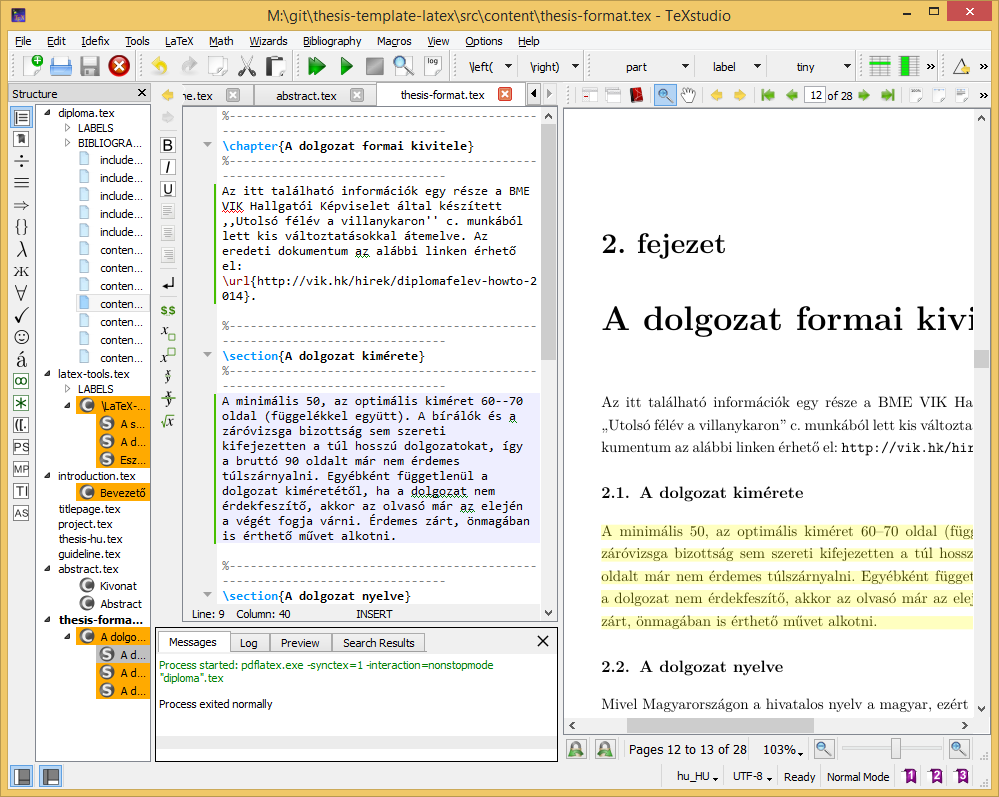
\includegraphics[width=67mm, keepaspectratio]{figures/TeXstudio.png}\hspace{1cm}
	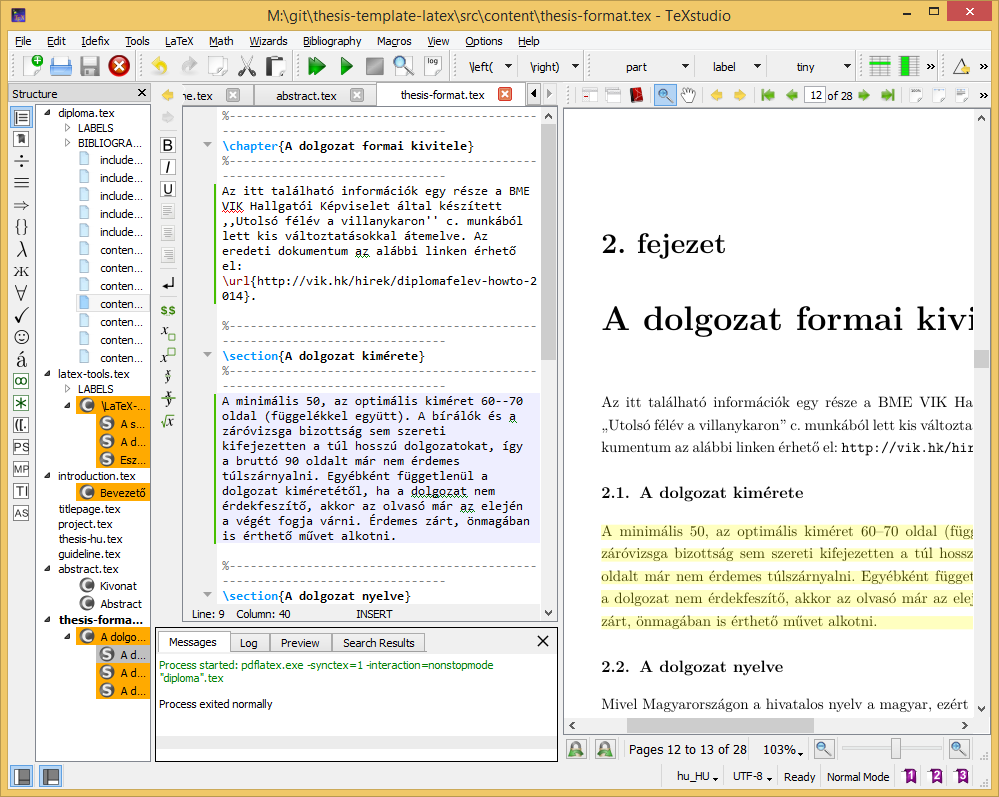
\includegraphics[width=67mm, keepaspectratio]{figures/TeXstudio.png}\\\vspace{5mm}
	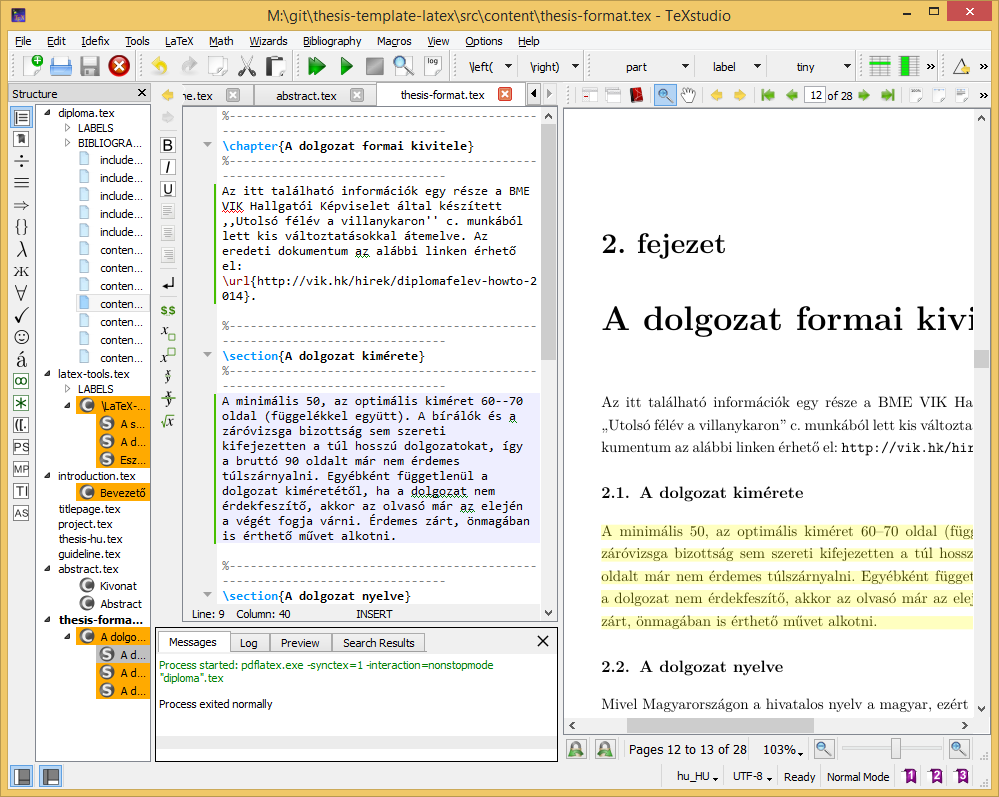
\includegraphics[width=67mm, keepaspectratio]{figures/TeXstudio.png}\hspace{1cm}
	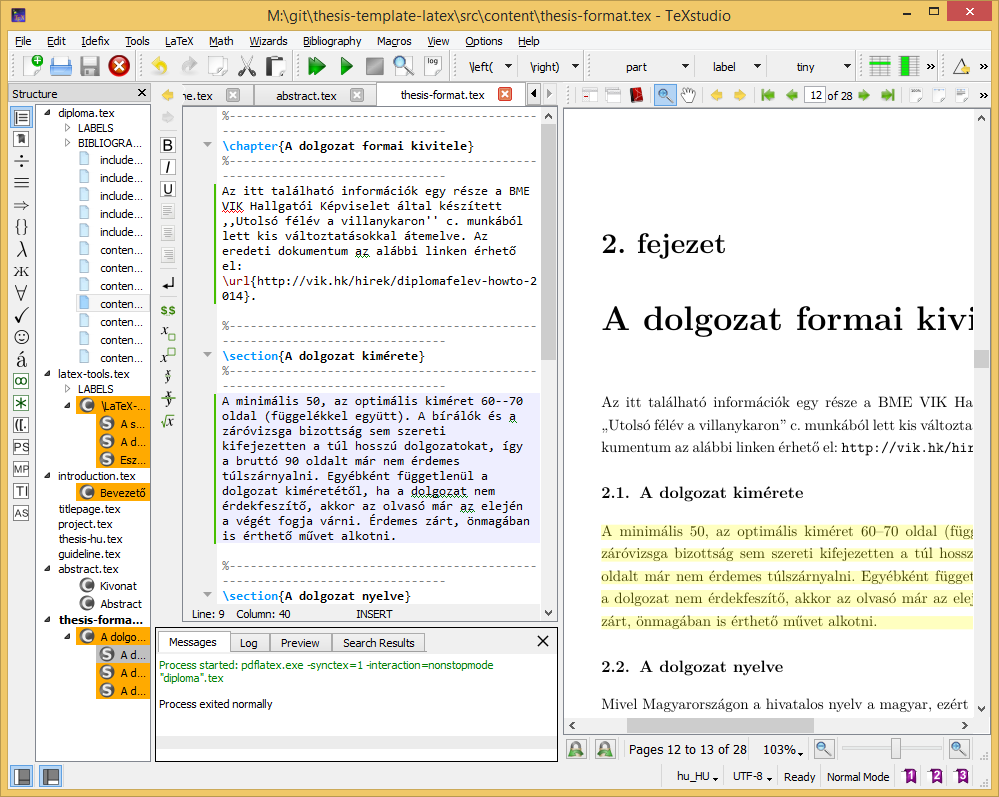
\includegraphics[width=67mm, keepaspectratio]{figures/TeXstudio.png}
	\caption{Több képfájl beillesztése esetén térközöket is érdemes használni.}
	\label{fig:HVSpaces}
\end{figure}

A táblázatok használatára \aref{tab:TabularExample}~táblázat mutat példát. A táblázatok formázásához hasznos tanácsokat találunk a \verb+booktabs+ csomag dokumentációjában.

\begin{table}[ht]
	\footnotesize
	\centering
	\begin{tabular}{ l c c }
		\toprule
		Órajel & Frekvencia & Cél pin \\
		\midrule
		CLKA & 100 MHz & FPGA CLK0\\
		CLKB & 48 MHz  & FPGA CLK1\\
		CLKC & 20 MHz  & Processzor\\
		CLKD & 25 MHz  & Ethernet chip \\
		CLKE & 72 MHz  & FPGA CLK2\\
		XBUF & 20 MHz  & FPGA CLK3\\
		\bottomrule
	\end{tabular}
	\caption{Az órajel-generátor chip órajel-kimenetei.}
	\label{tab:TabularExample}
\end{table}


%----------------------------------------------------------------------------
\section{Felsorolások és listák}
%----------------------------------------------------------------------------
Számozatlan felsorolásra mutat példát a jelenlegi bekezdés:
\begin{itemize}
	\item \emph{első bajusz:} ide lehetne írni az első elem kifejését,
	\item \emph{második bajusz:} ide lehetne írni a második elem kifejését,
	\item \emph{ez meg egy szakáll:} ide lehetne írni a harmadik elem kifejését.
\end{itemize}

Számozott felsorolást is készíthetünk az alábbi módon:
\begin{enumerate}
	\item \emph{első bajusz:} ide lehetne írni az első elem kifejését, és ez a kifejtés így néz ki, ha több sorosra sikeredik,
	\item \emph{második bajusz:} ide lehetne írni a második elem kifejését,
	\item \emph{ez meg egy szakáll:} ide lehetne írni a harmadik elem kifejését.
\end{enumerate}
A felsorolásokban sorok végén vessző, az utolsó sor végén pedig pont a szokásos írásjel. Ez alól kivételt képezhet, ha az egyes elemek több teljes mondatot tartalmaznak.

Listákban a dolgozat szövegétől elkülönítendő kódrészleteket, programsorokat, pszeudo-kódokat jeleníthetünk meg (\ref{lst:Example}.~kódrészlet).
\begin{lstlisting}[language=tex,caption=A fenti számozott felsorolás \LaTeX-forráskódja,label=lst:Example]
\begin{enumerate}
	\item \emph{els(*@ő@*) bajusz:} ide lehetne írni az els(*@ő@*) elem kifejését,
	és ez a kifejtés így néz ki, ha több sorosra sikeredik,
	\item \emph{második bajusz:} ide lehetne írni a második elem kifejését,
	\item \emph{ez meg egy szakáll:} ide lehetne írni a harmadik elem kifejését.
\end{enumerate}
\end{lstlisting}
A lista keretét, háttérszínét, egész stílusát megválaszthatjuk. Ráadásul különféle programnyelveket és a nyelveken belül kulcsszavakat is definiálhatunk, ha szükséges. Erről bővebbet a \verb+listings+ csomag hivatalos leírásában találhatunk.

%----------------------------------------------------------------------------
\section{Képletek}
%----------------------------------------------------------------------------
Ha egy formula nem túlságosan hosszú, és nem akarjuk hivatkozni a szövegből, mint például a $e^{i\pi}+1=0$ képlet, \emph{szövegközi képletként} szokás leírni. Csak, hogy másik példát is lássunk, az $U_i=-d\Phi/dt$ Faraday-törvény a $\rot E=-\frac{dB}{dt}$ differenciális alakban adott Maxwell-egyenlet felületre vett integráljából vezethető le. Látható, hogy a \LaTeX-fordító a sorközöket betartja, így a szöveg szedése esztétikus marad szövegközi képletek használata esetén is.

Képletek esetén az általános konvenció, hogy a kisbetűk skalárt, a kis félkövér betűk ($\mathbf{v}$) oszlopvektort -- és ennek megfelelően $\mathbf{v}^T$ sorvektort -- a kapitális félkövér betűk ($\mathbf{V}$) mátrixot jelölnek. Ha ettől el szeretnénk térni, akkor az alkalmazni kívánt jelölésmódot célszerű külön alfejezetben definiálni. Ennek megfelelően, amennyiben $\mathbf{y}$ jelöli a mérések vektorát, $\mathbf{\vartheta}$ a paraméterek vektorát és $\hat{\mathbf{y}}=\mathbf{X}\vartheta$ a paraméterekben lineáris modellt, akkor a \emph{Least-Squares} értelemben optimális paraméterbecslő $\hat{\mathbf{\vartheta}}_{LS}=(\mathbf{X}^T\mathbf{X})^{-1}\mathbf{X}^T\mathbf{y}$ lesz.

Emellett kiemelt, sorszámozott képleteket is megadhatunk, ennél az \verb+equation+ és a \verb+eqnarray+ környezetek helyett a korszerűbb \verb+align+ környezet alkalmazását javasoljuk (több okból, különféle problémák elkerülése végett, amelyekre most nem térünk ki). Tehát
\begin{align}
\dot{\mathbf{x}}&=\mathbf{A}\mathbf{x}+\mathbf{B}\mathbf{u},\\
\mathbf{y}&=\mathbf{C}\mathbf{x},
\end{align}
ahol $\mathbf{x}$ az állapotvektor, $\mathbf{y}$ a mérések vektora és $\mathbf{A}$, $\mathbf{B}$ és $\mathbf{C}$ a rendszert leíró paramétermátrixok. Figyeljük meg, hogy a két egyenletben az egyenlőségjelek egymáshoz igazítva jelennek meg, mivel a mindkettőt az \& karakter előzi meg a kódban. Lehetőség van számozatlan kiemelt képlet használatára is, például
\begin{align}
\dot{\mathbf{x}}&=\mathbf{A}\mathbf{x}+\mathbf{B}\mathbf{u},\nonumber\\
\mathbf{y}&=\mathbf{C}\mathbf{x}\nonumber.
\end{align}
Mátrixok felírására az $\mathbf{A}\mathbf{x}=\mathbf{b}$ inhomogén lineáris egyenlet részletes kifejtésével mutatunk példát:
\begin{align}
\begin{bmatrix}
a_{11} & a_{12} & \dots & a_{1n}\\
a_{21} & a_{22} & \dots & a_{2n}\\
\vdots & \vdots & \ddots & \vdots\\
a_{m1} & a_{m2} & \dots & a_{mn}
\end{bmatrix}
\begin{pmatrix}x_1\\x_2\\\vdots\\x_n\end{pmatrix}=
\begin{pmatrix}b_1\\b_2\\\vdots\\b_m\end{pmatrix}.
\end{align}
A \verb+\frac+ utasítás hatékonyságát egy általános másodfokú tag átviteli függvényén keresztül mutatjuk be, azaz
\begin{align}
W(s)=\frac{A}{1+2T\xi s+s^2T^2}.
\end{align}
A matematikai mód minden szimbólumának és képességének a bemutatására természetesen itt nincs lehetőség, de gyors referenciaként hatékonyan használhatók a következő linkek:\\
\indent\url{http://www.artofproblemsolving.com/LaTeX/AoPS_L_GuideSym.php},\\
\indent\url{http://www.ctan.org/tex-archive/info/symbols/comprehensive/symbols-a4.pdf},\\
\indent\url{ftp://ftp.ams.org/pub/tex/doc/amsmath/short-math-guide.pdf}.\\
Ez pedig itt egy magyarázat, hogy miért érdemes \verb+align+ környezetet használni:\\
\indent\url{http://texblog.net/latex-archive/maths/eqnarray-align-environment/}.

%----------------------------------------------------------------------------
\section{Irodalmi hivatkozások}
\label{sec:HowtoReference}
%----------------------------------------------------------------------------
Egy \LaTeX~dokumentumban az irodalmi hivatkozások definíciójának két módja van. Az egyik a \verb+\thebibliograhy+ környezet használata a dokumentum végén, az \verb+\end{document}+ lezárás előtt.
\begin{lstlisting}[language=tex]
\begin{thebibliography}{9}

\bibitem{Lamport94} Leslie Lamport, \emph{\LaTeX: A Document Preparation System}.
Addison Wesley, Massachusetts, 2nd Edition, 1994.

\end{thebibliography}
\end{lstlisting}

Ezek után a dokumentumban a \verb+\cite{Lamport94}+ utasítással hivatkozhatunk a forrásra. A fenti megadás viszonylag kötetlen, a szerző maga formázza az irodalomjegyzéket (ami gyakran inkonzisztens eredményhez vezet).

Egy sokkal professzionálisabb módszer a BiB\TeX{} használata, ezért ez a sablon is ezt támogatja. Ebben az esetben egy külön szöveges adatbázisban definiáljuk a forrásmunkákat, és egy külön stílusfájl határozza meg az irodalomjegyzék kinézetét. Ez, összhangban azzal, hogy külön formátumkonvenció határozza meg a folyóirat-, a könyv-, a konferenciacikk- stb. hivatkozások kinézetét az irodalomjegyzékben (a sablon használata esetén ezzel nem is kell foglalkoznia a hallgatónak, de az eredményt célszerű ellenőrizni). felhasznált hivatkozások adatbázisa egy \verb+.bib+ kiterjesztésű szöveges fájl, amelynek szerkezetét a \Aref{lst:Bibtex} kódrészlet demonstrálja. A forrásmunkák bevitelekor a sor végi vesszők külön figyelmet igényelnek, mert hiányuk a BiB\TeX-fordító hibaüzenetét eredményezi. A forrásmunkákat típus szerinti kulcsszó vezeti be (\verb+@book+ könyv, \verb+@inproceedings+ konferenciakiadványban megjelent cikk, \verb+@article+ folyóiratban megjelent cikk, \verb+@techreport+ valamelyik egyetem gondozásában megjelent műszaki tanulmány, \verb+@manual+ műszaki dokumentáció esetén stb.). Nemcsak a megjelenés stílusa, de a kötelezően megadandó mezők is típusról-típusra változnak. Egy jól használható referencia a \url{http://en.wikipedia.org/wiki/BibTeX} oldalon található.

\begin{lstlisting}[caption=Példa szöveges irodalomjegyzék-adatbázisra Bib\TeX{} használata esetén.,label=lst:Bibtex]
@book{Wettl04,
  author    = {Ferenc Wettl and Gyula Mayer and Péter Szabó},
  publisher = {Panem Könyvkiadó},
  title     = {\LaTeX~kézikönyv},
  year      = {2004},
}

@article{Candy86,
  author       = {James C. Candy},
  journaltitle = {{IEEE} Trans.\ on Communications},
  month        = {01},
  note         = {\doi{10.1109/TCOM.1986.1096432}},
  number       = {1},
  pages        = {72--76},
  title        = {Decimation for Sigma Delta Modulation},
  volume       = {34},
  year         = {1986},
}

@inproceedings{Lee87,
  author    = {Wai L. Lee and Charles G. Sodini},
  booktitle = {Proc.\ of the IEEE International Symposium on Circuits and Systems},
  location  = {Philadelphia, PA, USA},
  month     = {05~4--7},
  pages     = {459--462},
  title     = {A Topology for Higher Order Interpolative Coders},
  vol       = {2},
  year      = {1987},
}

@thesis{KissPhD,
  author      = {Peter Kiss},
  institution = {Technical University of Timi\c{s}oara, Romania},
  month       = {04},
  title       = {Adaptive Digital Compensation of Analog Circuit Imperfections for Cascaded Delta-Sigma Analog-to-Digital Converters},
  type        = {phdthesis},
  year        = {2000},
}

@manual{Schreier00,
  author       = {Richard Schreier},
  month        = {01},
  note         = {\url{http://www.mathworks.com/matlabcentral/fileexchange/}},
  organization = {Oregon State University},
  title        = {The Delta-Sigma Toolbox v5.2},
  year         = {2000},
}

@misc{DipPortal,
  author       = {{Budapesti Műszaki és Gazdaságtudományi Egyetem Villamosmérnöki és Informatikai Kar}},
  howpublished = {\url{http://diplomaterv.vik.bme.hu/}},
  title        = {Diplomaterv portál (2011. február 26.)},
}

@incollection{Mkrtychev:1997,
  author    = {Mkrtychev, Alexey},
  booktitle = {Logical Foundations of Computer Science},
  doi       = {10.1007/3-540-63045-7_27},
  editor    = {Adian, Sergei and Nerode, Anil},
  isbn      = {978-3-540-63045-6},
  pages     = {266-275},
  publisher = {Springer Berlin Heidelberg},
  series    = {Lecture Notes in Computer Science},
  title     = {Models for the logic of proofs},
  url       = {http://dx.doi.org/10.1007/3-540-63045-7_27},
  volume    = {1234},
  year      = {1997},
}
\end{lstlisting}

A stílusfájl egy \verb+.sty+ kiterjesztésű fájl, de ezzel lényegében nem kell foglalkozni, mert vannak beépített stílusok, amelyek jól használhatók. Ez a sablon a BiB\TeX-et használja, a hozzá tartozó adatbázisfájl a \verb+mybib.bib+ fájl. Megfigyelhető, hogy az irodalomjegyzéket a dokumentum végére (a \verb+\end{document}+ utasítás elé) beillesztett \verb+\bibliography{mybib}+ utasítással hozhatjuk létre, a stílusát pedig ugyanitt a  \verb+\bibliographystyle{plain}+ utasítással adhatjuk meg. Ebben az esetben a \verb+plain+ előre definiált stílust használjuk (a sablonban is ezt állítottuk be). A \verb+plain+ stíluson kívül természetesen számtalan más előre definiált stílus is létezik. Mivel a \verb+.bib+ adatbázisban ezeket megadtuk, a BiB\TeX-fordító is meg tudja különböztetni a szerzőt a címtől és a kiadótól, és ez alapján automatikusan generálódik az irodalomjegyzék a stílusfájl által meghatározott stílusban.

Az egyes forrásmunkákra a szövegből továbbra is a \verb+\cite+ paranccsal tudunk hivatkozni, így \aref{lst:Bibtex}.~kódrészlet esetén a hivatkozások rendre \verb+\cite{Wettl04}+, \verb+\cite{Candy86}+, \verb+\cite{Lee87}+, \verb+\cite{KissPhD}+, \verb+\cite{Schreirer00}+,
\verb+\cite{Mkrtychev:1997}+ és \verb+\cite{DipPortal}+. Az egyes forrásmunkák sorszáma az irodalomjegyzék bővítésekor változhat. Amennyiben az aktuális számhoz illeszkedő névelőt szeretnénk használni, használjuk az \verb+\acite{}+ parancsot.

Az irodalomjegyzékben alapértelmezésben csak azok a forrásmunkák jelennek meg, amelyekre található hivatkozás a szövegben, és ez így alapvetően helyes is, hiszen olyan forrásmunkákat nem illik az irodalomjegyzékbe írni, amelyekre nincs hivatkozás.

Mivel a fordítási folyamat során több lépésben oldódnak fel a szimbólumok, ezért gyakran többször is le kell fordítani a dokumentumot. Ilyenkor ez első 1-2 fordítás esetleg szimbólum-feloldásra vonatkozó figyelmeztető üzenettel zárul. Ha hibaüzenettel zárul bármelyik fordítás, akkor nincs értelme megismételni, hanem a hibát kell megkeresni. A \verb+.bib+ fájl megváltoztatáskor sokszor nincs hatása a változtatásnak azonnal, mivel nem mindig fut újra a BibTeX fordító. Ezért célszerű a változtatás után azt manuálisan is lefuttatni (TeXstudio esetén \verb+Tools/Bibliography+).

Hogy a szövegbe ágyazott hivatkozások kinézetét demonstráljuk, itt most sorban meghivatkozzuk a \cite{Wettl04}, \cite{Candy86}, \cite{Lee87}, \cite{KissPhD}, \cite{Schreier00} és \acite{Mkrtychev:1997}\footnote{Informatikai témában gyakran hivatkozunk cikkeket a Springer LNCS valamely kötetéből, ez a hivatkozás erre mutat egy helyes példát.} forrásmunkát, valamint \acite{DipPortal} weboldalt.

Megjegyzendő, hogy az ékezetes magyar betűket is tartalmazó \verb+.bib+ fájl az \verb+inputenc+ csomaggal betöltött \verb+latin2+ betűkészlet miatt fordítható. Ugyanez a \verb+.bib+ fájl hibaüzenettel fordul egy olyan dokumentumban, ami nem tartalmazza a \verb+\usepackage[latin2]{inputenc}+ sort. Speciális igény esetén az irodalmi adatbázis általánosabb érvényűvé tehető, ha az ékezetes betűket speciális latex karakterekkel helyettesítjük a \verb+.bib+ fájlban, pl. á helyett \verb+\'{a}+-t vagy ő helyett \verb+\H{o}+-t írunk.

Irodalomhivatkozásokat célszerű először olyan szolgáltatásokban keresni, ahol jó minőségű bejegyzések találhatók (pl. ACM Digital Library,\footnote{\url{https://dl.acm.org/}} DBLP,\footnote{\url{http://dblp.uni-trier.de/}} IEEE Xplore,\footnote{\url{http://ieeexplore.ieee.org/}} SpringerLink\footnote{\url{https://link.springer.com/}}) és csak ezek után használni kevésbé válogatott forrásokat (pl. Google Scholar\footnote{\url{http://scholar.google.com/}}). A jó minőségű bejegyzéseket is érdemes megfelelően tisztítani.\footnote{\url{https://github.com/FTSRG/cheat-sheets/wiki/BibTeX-Fixing-entries-from-common-sources}} A sablon angol nyelvű változatában használt \texttt{plainnat} beállítás egyik sajátossága, hogy a cikkhez generált hivatkozás a cikk DOI-ját és URL-jét is tartalmazza, ami gyakran duplikátumhoz vezet -- érdemes tehát a DOI-kat tartalmazó URL mezőket törölni. 

%----------------------------------------------------------------------------
\section{A dolgozat szerkezete és a forrásfájlok}
%----------------------------------------------------------------------------
A diplomatervsablonban a TeX fájlok két alkönyvtárban helyezkednek el. Az \verb+include+ könyvtárban azok szerepelnek, amiket tipikusan nem kell szerkesztenünk, ezek a sablon részei (pl. címoldal). A \verb+content+ alkönyvtárban pedig a saját munkánkat helyezhetjük el. Itt érdemes az egyes fejezeteket külön \TeX{} állományokba rakni.

A diplomatervsablon (a kari irányelvek szerint) az alábbi fő fejezetekből áll:
\begin{enumerate}
	\item 1 oldalas \emph{tájékoztató} a szakdolgozat/diplomaterv szerkezetéről (\verb+include/guideline.tex+), ami a végső dolgozatból törlendő,
	\item \emph{feladatkiírás} (\verb+include/project.tex+), a dolgozat nyomtatott verzójában ennek a helyére kerül a tanszék által kiadott, a tanszékvezető által aláírt feladatkiírás, a dolgozat elektronikus verziójába pedig a feladatkiírás egyáltalán ne kerüljön bele, azt külön tölti fel a tanszék a diplomaterv-honlapra,
	\item \emph{címoldal} (\verb+include/titlepage.tex+),
	\item \emph{tartalomjegyzék} (\verb+thesis.tex+),
	\item a diplomatervező \emph{nyilatkozat}a az önálló munkáról (\verb+include/declaration.tex+),
	\item 1-2 oldalas tartalmi \emph{összefoglaló} magyarul és angolul, illetve elkészíthető még további nyelveken is (\verb+content/abstract.tex+),
	\item \emph{bevezetés}: a feladat értelmezése, a tervezés célja, a feladat indokoltsága, a diplomaterv felépítésének rövid összefoglalása (\verb+content/introduction.tex+),
	\item sorszámmal ellátott \emph{fejezetek}: a feladatkiírás pontosítása és részletes elemzése, előzmények (irodalomkutatás, hasonló alkotások), az ezekből levonható következtetések, a tervezés részletes leírása, a döntési lehetőségek értékelése és a választott megoldások indoklása, a megtervezett műszaki alkotás értékelése, kritikai elemzése, továbbfejlesztési lehetőségek,
	\item esetleges \emph{köszönetnyilvánítás}ok (\verb+content/acknowledgement.tex+),
	\item részletes és pontos \emph{irodalomjegyzék} (ez a sablon esetében automatikusan generálódik a \verb+thesis.tex+ fájlban elhelyezett \verb+\bibliography+ utasítás hatására, \az+\refstruc{sec:HowtoReference}ban leírtak szerint),
	\item \emph{függelékek} (\verb+content/appendices.tex+).
\end{enumerate}

A sablonban a fejezetek a \verb+thesis.tex+ fájlba vannak beillesztve \verb+\include+ utasítások segítségével. Lehetőség van arra, hogy csak az éppen szerkesztés alatt álló \verb+.tex+ fájlt fordítsuk le, ezzel lerövidítve a fordítási folyamatot. Ezt a lehetőséget az alábbi kódrészlet biztosítja a \verb+thesis.tex+ fájlban.
\begin{lstlisting}
\includeonly{
	guideline,%
	project,%
	titlepage,%
	declaration,%
	abstract,%
	introduction,%
	chapter1,%
	chapter2,%
	chapter3,%
	acknowledgement,%
	appendices,%
}
\end{lstlisting}

Ha az alábbi kódrészletben az egyes sorokat a \verb+%+ szimbólummal kikommentezzük, akkor a megfelelő \verb+.tex+ fájl nem fordul le. Az oldalszámok és a tartalomjegyék természetesen csak akkor billennek helyre, ha a teljes dokumentumot lefordítjuk.

%----------------------------------------------------------------------------
\newpage
\section{Alapadatok megadása}
%----------------------------------------------------------------------------
A diplomaterv alapadatait (cím, szerző, konzulens, konzulens titulusa) a \verb+thesis.tex+ fájlban lehet megadni.

%----------------------------------------------------------------------------
\section{Új fejezet írása}
%----------------------------------------------------------------------------
A főfejezetek külön \verb+content+ könyvtárban foglalnak helyet. A sablonhoz 3 fejezet készült. További főfejezeteket úgy hozhatunk létre, ha új \TeX~fájlt készítünk a fejezet számára, és a \verb+thesis.tex+ fájlban, a \verb+\include+ és \verb+\includeonly+ utasítások argumentumába felvesszük az új \verb+.tex+ fájl nevét.


%----------------------------------------------------------------------------
\section{Definíciók, tételek, példák}
%----------------------------------------------------------------------------

\begin{definition}[Fluxuskondenzátor térerőssége]
Lorem ipsum dolor sit amet, consectetur adipiscing elit, sed do eiusmod tempor incididunt ut labore et dolore magna aliqua. Ut enim ad minim veniam, quis nostrud exercitation ullamco laboris nisi ut aliquip ex ea commodo consequat.
\end{definition}

\begin{example}
Példa egy példára. Duis aute irure dolor in reprehenderit in voluptate velit esse cillum dolore eu fugiat nulla pariatur. Excepteur sint occaecat cupidatat non proident, sunt in culpa qui officia deserunt mollit anim id est laborum.
\end{example}

\begin{theorem}[Kovács tétele]
Duis aute irure dolor in reprehenderit in voluptate velit esse cillum dolore eu fugiat nulla pariatur. Excepteur sint occaecat cupidatat non proident, sunt in culpa qui officia deserunt mollit anim id est laborum.
\end{theorem}



% Acknowledgements
%~~~~~~~~~~~~~~~~~~~~~~~~~~~~~~~~~~~~~~~~~~~~~~~~~~~~~~~~~~~~~~~~~~~~~~~~~~~~~~~~~~~~~~
%----------------------------------------------------------------------------
\chapter*{\koszonetnyilvanitas}\addcontentsline{toc}{chapter}{\koszonetnyilvanitas}
%----------------------------------------------------------------------------

%Ez nem kötelező, akár törölhető is. Ha a szerző szükségét érzi, itt lehet köszönetet nyilvánítani azoknak, akik hozzájárultak munkájukkal ahhoz, hogy a hallgató a szakdolgozatban vagy diplomamunkában leírt feladatokat sikeresen elvégezze. A konzulensnek való köszönetnyilvánítás sem kötelező, a konzulensnek hivatalosan is dolga, hogy a hallgatót konzultálja.

This work was supported in part by the Kormányzati Informatikai Fejleszési Ügynökség (KIFÜ). KIFÜ provided a 150 GPU hours to the project on the Komondor high per- formance computing (HPC) cluster, which was utilized in the discovery process of the  methodology.

First, I would like to thank our mentor, Dr. Bertalan Forstner, for his valuable advice and support throughout the project.

I appreciate the work of Máté Debreczeni, the idea's originator and the creator of the AI-related features. Without him, the platform could not have been built.

And last but not least, I would like to thank Dr. Imre Szeberényi for his help with the Komondor application.


% List of Figures, Tables
%~~~~~~~~~~~~~~~~~~~~~~~~~~~~~~~~~~~~~~~~~~~~~~~~~~~~~~~~~~~~~~~~~~~~~~~~~~~~~~~~~~~~~~
%\listoffigures\addcontentsline{toc}{chapter}{\listfigurename}
%\listoftables\addcontentsline{toc}{chapter}{\listtablename}


% Bibliography
%~~~~~~~~~~~~~~~~~~~~~~~~~~~~~~~~~~~~~~~~~~~~~~~~~~~~~~~~~~~~~~~~~~~~~~~~~~~~~~~~~~~~~~
\addcontentsline{toc}{chapter}{\bibname}
\bibliography{bib/mybib}


% Appendix
%~~~~~~~~~~~~~~~~~~~~~~~~~~~~~~~~~~~~~~~~~~~~~~~~~~~~~~~~~~~~~~~~~~~~~~~~~~~~~~~~~~~~~~
%----------------------------------------------------------------------------
\appendix
%----------------------------------------------------------------------------
\chapter*{\fuggelek}\addcontentsline{toc}{chapter}{\fuggelek}
\setcounter{chapter}{\appendixnumber}
%\setcounter{equation}{0} % a fofejezet-szamlalo az angol ABC 6. betuje (F) lesz
\numberwithin{equation}{section}
\numberwithin{figure}{section}
\numberwithin{lstlisting}{section}
%\numberwithin{tabular}{section}

%TODO innentől spam

%----------------------------------------------------------------------------
%\section{A TeXstudio felülete}
%----------------------------------------------------------------------------
%\begin{figure}[!ht]
%\centering
%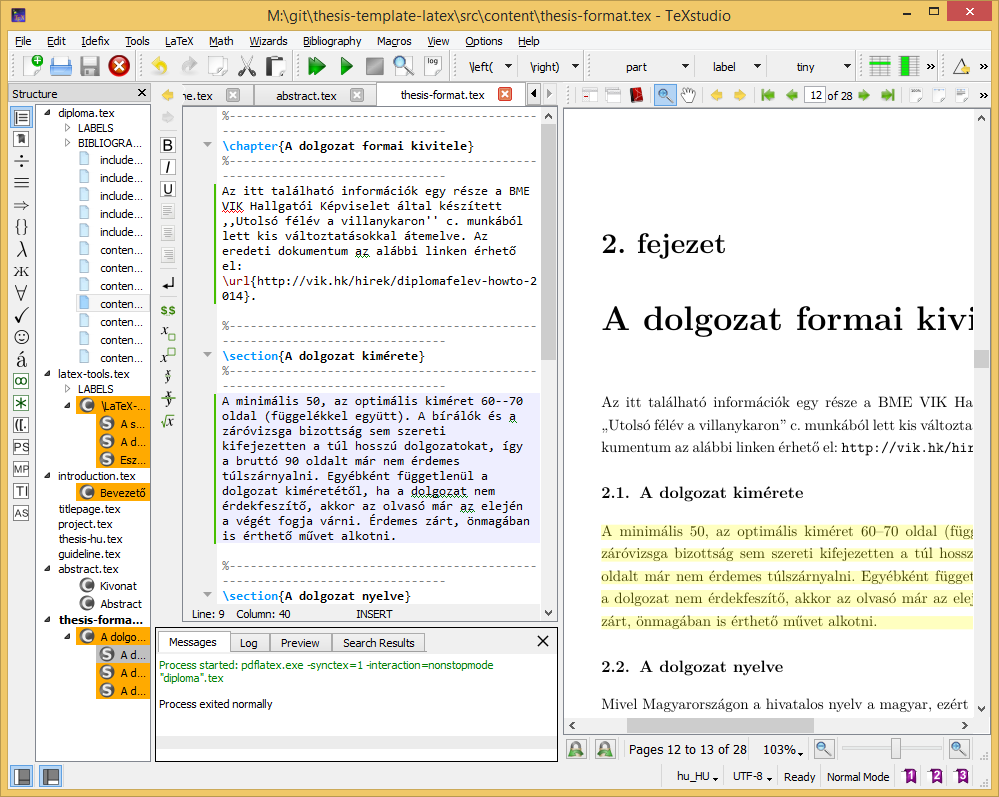
\includegraphics[width=150mm, keepaspectratio]{figures/TeXstudio.png}
%\caption{A TeXstudio \LaTeX-szerkesztő.} 
%\end{figure}

%----------------------------------------------------------------------------
%\clearpage\section{Válasz az ,,Élet, a világmindenség, meg minden'' kérdésére}
%----------------------------------------------------------------------------
%A Pitagorasz-tételből levezetve
%\begin{align}
%c^2=a^2+b^2=42.
%\end{align}
%A Faraday-indukciós törvényből levezetve
%\begin{align}
%\rot E=-\frac{dB}{dt}\hspace{1cm}\longrightarrow \hspace{1cm}
%U_i=\oint\limits_\mathbf{L}{\mathbf{E}\mathbf{dl}}=-\frac{d}%{dt}\int\limits_A{\mathbf{B}\mathbf{da}}=42.
%\end{align}


%\label{page:last}
\end{document}
